\documentclass[twoside]{book}

% Packages required by doxygen
\usepackage{fixltx2e}
\usepackage{calc}
\usepackage{doxygen}
\usepackage{graphicx}
\usepackage[utf8]{inputenc}
\usepackage{makeidx}
\usepackage{multicol}
\usepackage{multirow}
\PassOptionsToPackage{warn}{textcomp}
\usepackage{textcomp}
\usepackage[nointegrals]{wasysym}
\usepackage[table]{xcolor}

% Font selection
\usepackage[T1]{fontenc}
\usepackage{mathptmx}
\usepackage[scaled=.90]{helvet}
\usepackage{courier}
\usepackage{amssymb}
\usepackage{sectsty}
\renewcommand{\familydefault}{\sfdefault}
\allsectionsfont{%
  \fontseries{bc}\selectfont%
  \color{darkgray}%
}
\renewcommand{\DoxyLabelFont}{%
  \fontseries{bc}\selectfont%
  \color{darkgray}%
}
\newcommand{\+}{\discretionary{\mbox{\scriptsize$\hookleftarrow$}}{}{}}

% Page & text layout
\usepackage{geometry}
\geometry{%
  a4paper,%
  top=2.5cm,%
  bottom=2.5cm,%
  left=2.5cm,%
  right=2.5cm%
}
\tolerance=750
\hfuzz=15pt
\hbadness=750
\setlength{\emergencystretch}{15pt}
\setlength{\parindent}{0cm}
\setlength{\parskip}{0.2cm}
\makeatletter
\renewcommand{\paragraph}{%
  \@startsection{paragraph}{4}{0ex}{-1.0ex}{1.0ex}{%
    \normalfont\normalsize\bfseries\SS@parafont%
  }%
}
\renewcommand{\subparagraph}{%
  \@startsection{subparagraph}{5}{0ex}{-1.0ex}{1.0ex}{%
    \normalfont\normalsize\bfseries\SS@subparafont%
  }%
}
\makeatother

% Headers & footers
\usepackage{fancyhdr}
\pagestyle{fancyplain}
\fancyhead[LE]{\fancyplain{}{\bfseries\thepage}}
\fancyhead[CE]{\fancyplain{}{}}
\fancyhead[RE]{\fancyplain{}{\bfseries\leftmark}}
\fancyhead[LO]{\fancyplain{}{\bfseries\rightmark}}
\fancyhead[CO]{\fancyplain{}{}}
\fancyhead[RO]{\fancyplain{}{\bfseries\thepage}}
\fancyfoot[LE]{\fancyplain{}{}}
\fancyfoot[CE]{\fancyplain{}{}}
\fancyfoot[RE]{\fancyplain{}{\bfseries\scriptsize Generated on Thu Nov 19 2015 12\+:23\+:21 for My Project by Doxygen }}
\fancyfoot[LO]{\fancyplain{}{\bfseries\scriptsize Generated on Thu Nov 19 2015 12\+:23\+:21 for My Project by Doxygen }}
\fancyfoot[CO]{\fancyplain{}{}}
\fancyfoot[RO]{\fancyplain{}{}}
\renewcommand{\footrulewidth}{0.4pt}
\renewcommand{\chaptermark}[1]{%
  \markboth{#1}{}%
}
\renewcommand{\sectionmark}[1]{%
  \markright{\thesection\ #1}%
}

% Indices & bibliography
\usepackage{natbib}
\usepackage[titles]{tocloft}
\setcounter{tocdepth}{3}
\setcounter{secnumdepth}{5}
\makeindex

% Hyperlinks (required, but should be loaded last)
\usepackage{ifpdf}
\ifpdf
  \usepackage[pdftex,pagebackref=true]{hyperref}
\else
  \usepackage[ps2pdf,pagebackref=true]{hyperref}
\fi
\hypersetup{%
  colorlinks=true,%
  linkcolor=blue,%
  citecolor=blue,%
  unicode%
}

% Custom commands
\newcommand{\clearemptydoublepage}{%
  \newpage{\pagestyle{empty}\cleardoublepage}%
}


%===== C O N T E N T S =====

\begin{document}

% Titlepage & ToC
\hypersetup{pageanchor=false,
             bookmarks=true,
             bookmarksnumbered=true,
             pdfencoding=unicode
            }
\pagenumbering{roman}
\begin{titlepage}
\vspace*{7cm}
\begin{center}%
{\Large My Project }\\
\vspace*{1cm}
{\large Generated by Doxygen 1.8.7}\\
\vspace*{0.5cm}
{\small Thu Nov 19 2015 12:23:21}\\
\end{center}
\end{titlepage}
\clearemptydoublepage
\tableofcontents
\clearemptydoublepage
\pagenumbering{arabic}
\hypersetup{pageanchor=true}

%--- Begin generated contents ---
\chapter{Hierarchical Index}
\section{Class Hierarchy}
This inheritance list is sorted roughly, but not completely, alphabetically\+:\begin{DoxyCompactList}
\item \contentsline{section}{A\+I}{\pageref{class_a_i}}{}
\begin{DoxyCompactList}
\item \contentsline{section}{A\+I\+\_\+\+Boomer}{\pageref{class_a_i___boomer}}{}
\item \contentsline{section}{A\+I\+\_\+\+Follower}{\pageref{class_a_i___follower}}{}
\item \contentsline{section}{A\+I\+\_\+\+Jumper}{\pageref{class_a_i___jumper}}{}
\item \contentsline{section}{A\+I\+\_\+\+Land\+Base}{\pageref{class_a_i___land_base}}{}
\end{DoxyCompactList}
\item \contentsline{section}{Alive\+Entity}{\pageref{class_alive_entity}}{}
\begin{DoxyCompactList}
\item \contentsline{section}{Enemy}{\pageref{class_enemy}}{}
\begin{DoxyCompactList}
\item \contentsline{section}{Boomer}{\pageref{class_boomer}}{}
\item \contentsline{section}{Jumper}{\pageref{class_jumper}}{}
\end{DoxyCompactList}
\item \contentsline{section}{Personnage}{\pageref{class_personnage}}{}
\end{DoxyCompactList}
\item Drawable\begin{DoxyCompactList}
\item \contentsline{section}{Jeu}{\pageref{class_jeu}}{}
\item \contentsline{section}{State}{\pageref{class_state}}{}
\begin{DoxyCompactList}
\item \contentsline{section}{State\+Esc\+Menu}{\pageref{class_state_esc_menu}}{}
\item \contentsline{section}{State\+Level}{\pageref{class_state_level}}{}
\item \contentsline{section}{State\+Main\+Menu}{\pageref{class_state_main_menu}}{}
\item \contentsline{section}{State\+Stats}{\pageref{class_state_stats}}{}
\end{DoxyCompactList}
\item \contentsline{section}{Tile\+Map}{\pageref{class_tile_map}}{}
\end{DoxyCompactList}
\item \contentsline{section}{Spawner}{\pageref{class_spawner}}{}
\item Transformable\begin{DoxyCompactList}
\item \contentsline{section}{Jeu}{\pageref{class_jeu}}{}
\item \contentsline{section}{State}{\pageref{class_state}}{}
\item \contentsline{section}{Tile\+Map}{\pageref{class_tile_map}}{}
\end{DoxyCompactList}
\end{DoxyCompactList}

\chapter{Class Index}
\section{Class List}
Here are the classes, structs, unions and interfaces with brief descriptions\+:\begin{DoxyCompactList}
\item\contentsline{section}{\hyperlink{class_a_i}{A\+I} \\*Classe abstraites pour les I\+A des ennemis }{\pageref{class_a_i}}{}
\item\contentsline{section}{\hyperlink{class_a_i___boomer}{A\+I\+\_\+\+Boomer} \\*Classe gérant l'\hyperlink{class_a_i}{A\+I} des ennemi qui sautent }{\pageref{class_a_i___boomer}}{}
\item\contentsline{section}{\hyperlink{class_a_i___follower}{A\+I\+\_\+\+Follower} \\*Classe gérant l'\hyperlink{class_a_i}{A\+I} des ennemi qui sautent }{\pageref{class_a_i___follower}}{}
\item\contentsline{section}{\hyperlink{class_a_i___jumper}{A\+I\+\_\+\+Jumper} \\*Classe gérant l'\hyperlink{class_a_i}{A\+I} des ennemi qui sautent }{\pageref{class_a_i___jumper}}{}
\item\contentsline{section}{\hyperlink{class_a_i___land_base}{A\+I\+\_\+\+Land\+Base} \\*Classe gérant l'\hyperlink{class_a_i}{A\+I} des ennemi qui marchent }{\pageref{class_a_i___land_base}}{}
\item\contentsline{section}{\hyperlink{class_alive_entity}{Alive\+Entity} \\*Classe abstraite qui définissant les objets \char`\"{}vivants\char`\"{} }{\pageref{class_alive_entity}}{}
\item\contentsline{section}{\hyperlink{class_boomer}{Boomer} \\*Classe gérant les ennemi qui explosent et se devisent }{\pageref{class_boomer}}{}
\item\contentsline{section}{\hyperlink{class_enemy}{Enemy} \\*Classe abstraite qui définissant les objets \char`\"{}vivants\char`\"{} }{\pageref{class_enemy}}{}
\item\contentsline{section}{\hyperlink{class_jeu}{Jeu} \\*Gère tout la fenêtre et les interactions lors d'une partie }{\pageref{class_jeu}}{}
\item\contentsline{section}{\hyperlink{class_jumper}{Jumper} \\*Classe gérant les ennemi qui marchent }{\pageref{class_jumper}}{}
\item\contentsline{section}{\hyperlink{class_personnage}{Personnage} \\*Classe définissant un personnage }{\pageref{class_personnage}}{}
\item\contentsline{section}{\hyperlink{class_spawner}{Spawner} }{\pageref{class_spawner}}{}
\item\contentsline{section}{\hyperlink{class_state}{State} \\*Interface du \hyperlink{class_state}{State} }{\pageref{class_state}}{}
\item\contentsline{section}{\hyperlink{class_state_esc_menu}{State\+Esc\+Menu} \\*Etat Esc\+Menu rattaché au Pattern \hyperlink{class_state}{State} }{\pageref{class_state_esc_menu}}{}
\item\contentsline{section}{\hyperlink{class_state_level}{State\+Level} \\*Etat \hyperlink{class_state_level}{State\+Level} rattaché au Pattern \hyperlink{class_state}{State} }{\pageref{class_state_level}}{}
\item\contentsline{section}{\hyperlink{class_state_main_menu}{State\+Main\+Menu} \\*Etat Main\+Menu rattaché au Pattern \hyperlink{class_state}{State} }{\pageref{class_state_main_menu}}{}
\item\contentsline{section}{\hyperlink{class_state_stats}{State\+Stats} \\*Etat \hyperlink{class_state_stats}{State\+Stats} rattaché au Pattern \hyperlink{class_state}{State} }{\pageref{class_state_stats}}{}
\item\contentsline{section}{\hyperlink{class_tile_map}{Tile\+Map} \\*Classe définissant un map }{\pageref{class_tile_map}}{}
\end{DoxyCompactList}

\chapter{File Index}
\section{File List}
Here is a list of all documented files with brief descriptions\+:\begin{DoxyCompactList}
\item\contentsline{section}{\hyperlink{_a_i_8hpp}{A\+I.\+hpp} \\*Pattern Stratégie gérant les I\+A des ennemis }{\pageref{_a_i_8hpp}}{}
\item\contentsline{section}{\hyperlink{_a_i___boomer_8hpp}{A\+I\+\_\+\+Boomer.\+hpp} \\*\hyperlink{class_a_i}{A\+I} des boomers }{\pageref{_a_i___boomer_8hpp}}{}
\item\contentsline{section}{\hyperlink{_a_i___follower_8hpp}{A\+I\+\_\+\+Follower.\+hpp} \\*\hyperlink{class_a_i}{A\+I} des enemy sautant }{\pageref{_a_i___follower_8hpp}}{}
\item\contentsline{section}{\hyperlink{_a_i___jumper_8hpp}{A\+I\+\_\+\+Jumper.\+hpp} \\*\hyperlink{class_a_i}{A\+I} des enemy sautant }{\pageref{_a_i___jumper_8hpp}}{}
\item\contentsline{section}{\hyperlink{_a_i___land_base_8hpp}{A\+I\+\_\+\+Land\+Base.\+hpp} \\*\hyperlink{class_a_i}{A\+I} des enemy au sol }{\pageref{_a_i___land_base_8hpp}}{}
\item\contentsline{section}{\hyperlink{_alive_entity_8hpp}{Alive\+Entity.\+hpp} \\*Classe définissant les objets \char`\"{}vivants\char`\"{} }{\pageref{_alive_entity_8hpp}}{}
\item\contentsline{section}{\hyperlink{_boomer_8hpp}{Boomer.\+hpp} \\*Classe des ennemis qui grossissent puis explosent }{\pageref{_boomer_8hpp}}{}
\item\contentsline{section}{\hyperlink{_enemy_8hpp}{Enemy.\+hpp} \\*Classe définissant les ennemis }{\pageref{_enemy_8hpp}}{}
\item\contentsline{section}{\hyperlink{_jeu_8hpp}{Jeu.\+hpp} \\*Gère l'ensemble des outils permettant d'effectuer une partie de Ducky\+Duck }{\pageref{_jeu_8hpp}}{}
\item\contentsline{section}{\hyperlink{_jumper_8hpp}{Jumper.\+hpp} \\*Classe des ennemis marchant }{\pageref{_jumper_8hpp}}{}
\item\contentsline{section}{\hyperlink{_personnage_8hpp}{Personnage.\+hpp} \\*Gère l'ensemble des outils neccessaires à l'éxécution des différentes méthodes du personnage }{\pageref{_personnage_8hpp}}{}
\item\contentsline{section}{\hyperlink{_spawner_8hpp}{Spawner.\+hpp} \\*Créer une instance de \hyperlink{class_enemy}{Enemy} }{\pageref{_spawner_8hpp}}{}
\item\contentsline{section}{\hyperlink{_state_8hpp}{State.\+hpp} \\*\hyperlink{class_state}{State} }{\pageref{_state_8hpp}}{}
\item\contentsline{section}{\hyperlink{_state_esc_menu_8hpp}{State\+Esc\+Menu.\+hpp} \\*Menu Pause du jeu }{\pageref{_state_esc_menu_8hpp}}{}
\item\contentsline{section}{\hyperlink{_state_level_8hpp}{State\+Level.\+hpp} \\*Etat en jeu }{\pageref{_state_level_8hpp}}{}
\item\contentsline{section}{\hyperlink{_state_main_menu_8hpp}{State\+Main\+Menu.\+hpp} \\*Menu principal }{\pageref{_state_main_menu_8hpp}}{}
\item\contentsline{section}{\hyperlink{_state_stats_8hpp}{State\+Stats.\+hpp} \\*Affichage en fin de niveau }{\pageref{_state_stats_8hpp}}{}
\item\contentsline{section}{\hyperlink{_tile_map_8hpp}{Tile\+Map.\+hpp} \\*Gère les différentes interactions avec la map }{\pageref{_tile_map_8hpp}}{}
\end{DoxyCompactList}

\chapter{Class Documentation}
\hypertarget{class_a_i}{\section{A\+I Class Reference}
\label{class_a_i}\index{A\+I@{A\+I}}
}


Classe abstraites pour les I\+A des ennemis.  




{\ttfamily \#include $<$A\+I.\+hpp$>$}



Inheritance diagram for A\+I\+:
\nopagebreak
\begin{figure}[H]
\begin{center}
\leavevmode
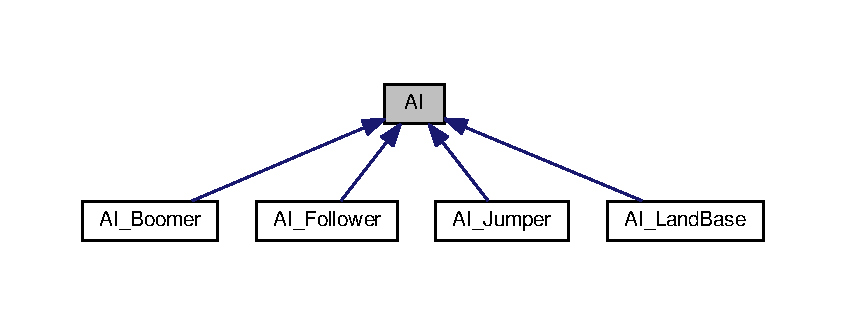
\includegraphics[width=350pt]{class_a_i__inherit__graph}
\end{center}
\end{figure}


Collaboration diagram for A\+I\+:
\nopagebreak
\begin{figure}[H]
\begin{center}
\leavevmode
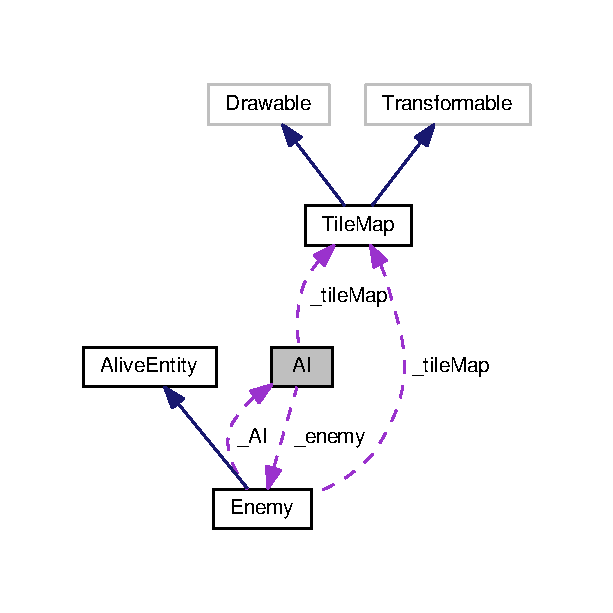
\includegraphics[width=294pt]{class_a_i__coll__graph}
\end{center}
\end{figure}
\subsection*{Public Member Functions}
\begin{DoxyCompactItemize}
\item 
\hyperlink{class_a_i_ac6a30583e7e676d85434d7e88eeec041}{A\+I} (\hyperlink{class_enemy}{Enemy} $\ast$enemy, const \hyperlink{class_tile_map}{Tile\+Map} \&tilemap)
\begin{DoxyCompactList}\small\item\em Constructeur. \end{DoxyCompactList}\item 
virtual \hyperlink{class_a_i_ac86c87957e3d563f6ea2137a97992e0a}{$\sim$\+A\+I} ()
\begin{DoxyCompactList}\small\item\em Destructeur. \end{DoxyCompactList}\item 
virtual void \hyperlink{class_a_i_a029ec0ca07e6644af6662cf08300ed0c}{move} ()=0
\begin{DoxyCompactList}\small\item\em Procédure gérant le mouvement de l'ennemi. \end{DoxyCompactList}\end{DoxyCompactItemize}
\subsection*{Protected Attributes}
\begin{DoxyCompactItemize}
\item 
\hypertarget{class_a_i_af918afabc099ef611231be287eb4d6df}{\hyperlink{class_enemy}{Enemy} $\ast$ {\bfseries \+\_\+enemy}}\label{class_a_i_af918afabc099ef611231be287eb4d6df}

\item 
const \hyperlink{class_tile_map}{Tile\+Map} \& \hyperlink{class_a_i_a5b798605999a06067b97a45c6e7f2dc2}{\+\_\+tile\+Map}
\end{DoxyCompactItemize}


\subsection{Detailed Description}
Classe abstraites pour les I\+A des ennemis. 

\subsection{Constructor \& Destructor Documentation}
\hypertarget{class_a_i_ac6a30583e7e676d85434d7e88eeec041}{\index{A\+I@{A\+I}!A\+I@{A\+I}}
\index{A\+I@{A\+I}!A\+I@{A\+I}}
\subsubsection[{A\+I}]{\setlength{\rightskip}{0pt plus 5cm}A\+I\+::\+A\+I (
\begin{DoxyParamCaption}
\item[{{\bf Enemy} $\ast$}]{enemy, }
\item[{const {\bf Tile\+Map} \&}]{tilemap}
\end{DoxyParamCaption}
)}}\label{class_a_i_ac6a30583e7e676d85434d7e88eeec041}


Constructeur. 

Constructeur de la classe \hyperlink{class_a_i}{A\+I}


\begin{DoxyParams}{Parameters}
{\em enemy} & \+: Ennemi utilisant l'I\+A, tilemap \+: tilemap sur laquelle l'enemy est. \\
\hline
\end{DoxyParams}
\hypertarget{class_a_i_ac86c87957e3d563f6ea2137a97992e0a}{\index{A\+I@{A\+I}!````~A\+I@{$\sim$\+A\+I}}
\index{````~A\+I@{$\sim$\+A\+I}!A\+I@{A\+I}}
\subsubsection[{$\sim$\+A\+I}]{\setlength{\rightskip}{0pt plus 5cm}virtual A\+I\+::$\sim$\+A\+I (
\begin{DoxyParamCaption}
{}
\end{DoxyParamCaption}
)\hspace{0.3cm}{\ttfamily [virtual]}}}\label{class_a_i_ac86c87957e3d563f6ea2137a97992e0a}


Destructeur. 

Destructeur de la classe \hyperlink{class_a_i}{A\+I} 

\subsection{Member Function Documentation}
\hypertarget{class_a_i_a029ec0ca07e6644af6662cf08300ed0c}{\index{A\+I@{A\+I}!move@{move}}
\index{move@{move}!A\+I@{A\+I}}
\subsubsection[{move}]{\setlength{\rightskip}{0pt plus 5cm}void A\+I\+::move (
\begin{DoxyParamCaption}
{}
\end{DoxyParamCaption}
)\hspace{0.3cm}{\ttfamily [pure virtual]}}}\label{class_a_i_a029ec0ca07e6644af6662cf08300ed0c}


Procédure gérant le mouvement de l'ennemi. 

Procédure qui permet de mouvoir l'ennemi en fonction de l'\hyperlink{class_a_i}{A\+I} qu'il a adopter 

Implemented in \hyperlink{class_a_i___follower_a37893e7aa601169682333af093235c13}{A\+I\+\_\+\+Follower}, \hyperlink{class_a_i___boomer_a7fc6dbcfbc0a2aa557614bfb47935df6}{A\+I\+\_\+\+Boomer}, \hyperlink{class_a_i___jumper_a49e2ba05ef7f14020faf4f521370dbfa}{A\+I\+\_\+\+Jumper}, and \hyperlink{class_a_i___land_base_af536a9f2a45fd52189542761bcf285d4}{A\+I\+\_\+\+Land\+Base}.



\subsection{Member Data Documentation}
\hypertarget{class_a_i_a5b798605999a06067b97a45c6e7f2dc2}{\index{A\+I@{A\+I}!\+\_\+tile\+Map@{\+\_\+tile\+Map}}
\index{\+\_\+tile\+Map@{\+\_\+tile\+Map}!A\+I@{A\+I}}
\subsubsection[{\+\_\+tile\+Map}]{\setlength{\rightskip}{0pt plus 5cm}const {\bf Tile\+Map}\& A\+I\+::\+\_\+tile\+Map\hspace{0.3cm}{\ttfamily [protected]}}}\label{class_a_i_a5b798605999a06067b97a45c6e7f2dc2}
Ennemi qui utilise l'\hyperlink{class_a_i}{A\+I} 

The documentation for this class was generated from the following file\+:\begin{DoxyCompactItemize}
\item 
\hyperlink{_a_i_8hpp}{A\+I.\+hpp}\end{DoxyCompactItemize}

\hypertarget{class_a_i___boomer}{\section{A\+I\+\_\+\+Boomer Class Reference}
\label{class_a_i___boomer}\index{A\+I\+\_\+\+Boomer@{A\+I\+\_\+\+Boomer}}
}


Classe gérant l'\hyperlink{class_a_i}{A\+I} des ennemi qui sautent.  




{\ttfamily \#include $<$A\+I\+\_\+\+Boomer.\+hpp$>$}



Inheritance diagram for A\+I\+\_\+\+Boomer\+:
\nopagebreak
\begin{figure}[H]
\begin{center}
\leavevmode
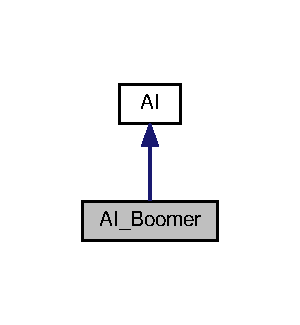
\includegraphics[width=144pt]{class_a_i___boomer__inherit__graph}
\end{center}
\end{figure}


Collaboration diagram for A\+I\+\_\+\+Boomer\+:
\nopagebreak
\begin{figure}[H]
\begin{center}
\leavevmode
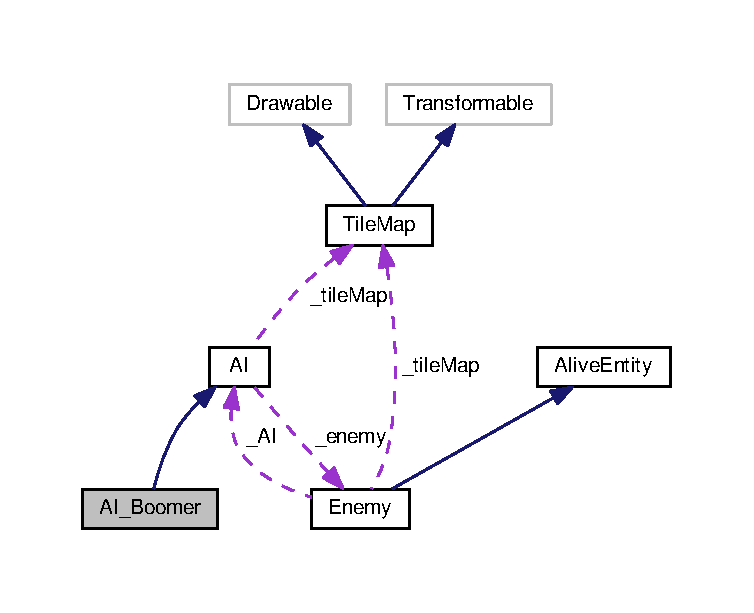
\includegraphics[width=350pt]{class_a_i___boomer__coll__graph}
\end{center}
\end{figure}
\subsection*{Public Member Functions}
\begin{DoxyCompactItemize}
\item 
\hyperlink{class_a_i___boomer_a72fd0c6e03925f54c1b76a5e879a2a07}{A\+I\+\_\+\+Boomer} (\hyperlink{class_boomer}{Boomer} $\ast$\hyperlink{class_boomer}{Boomer}, const \hyperlink{class_tile_map}{Tile\+Map} \&tilemap)
\begin{DoxyCompactList}\small\item\em Constructeur. \end{DoxyCompactList}\item 
virtual void \hyperlink{class_a_i___boomer_a7fc6dbcfbc0a2aa557614bfb47935df6}{move} ()
\begin{DoxyCompactList}\small\item\em Procédure gérant le mouvement de l'ennemi. \end{DoxyCompactList}\end{DoxyCompactItemize}
\subsection*{Additional Inherited Members}


\subsection{Detailed Description}
Classe gérant l'\hyperlink{class_a_i}{A\+I} des ennemi qui sautent. 

\subsection{Constructor \& Destructor Documentation}
\hypertarget{class_a_i___boomer_a72fd0c6e03925f54c1b76a5e879a2a07}{\index{A\+I\+\_\+\+Boomer@{A\+I\+\_\+\+Boomer}!A\+I\+\_\+\+Boomer@{A\+I\+\_\+\+Boomer}}
\index{A\+I\+\_\+\+Boomer@{A\+I\+\_\+\+Boomer}!A\+I\+\_\+\+Boomer@{A\+I\+\_\+\+Boomer}}
\subsubsection[{A\+I\+\_\+\+Boomer}]{\setlength{\rightskip}{0pt plus 5cm}A\+I\+\_\+\+Boomer\+::\+A\+I\+\_\+\+Boomer (
\begin{DoxyParamCaption}
\item[{{\bf Boomer} $\ast$}]{Boomer, }
\item[{const {\bf Tile\+Map} \&}]{tilemap}
\end{DoxyParamCaption}
)}}\label{class_a_i___boomer_a72fd0c6e03925f54c1b76a5e879a2a07}


Constructeur. 

Constructeur de la classe \hyperlink{class_a_i___boomer}{A\+I\+\_\+\+Boomer}.


\begin{DoxyParams}{Parameters}
{\em enemy} & \+: Ennemi utilisant l'I\+A, tilemap \+: \hyperlink{class_tile_map}{Tile\+Map} sur laquelle l'\hyperlink{class_enemy}{Enemy} est. \\
\hline
\end{DoxyParams}


\subsection{Member Function Documentation}
\hypertarget{class_a_i___boomer_a7fc6dbcfbc0a2aa557614bfb47935df6}{\index{A\+I\+\_\+\+Boomer@{A\+I\+\_\+\+Boomer}!move@{move}}
\index{move@{move}!A\+I\+\_\+\+Boomer@{A\+I\+\_\+\+Boomer}}
\subsubsection[{move}]{\setlength{\rightskip}{0pt plus 5cm}void A\+I\+\_\+\+Boomer\+::move (
\begin{DoxyParamCaption}
{}
\end{DoxyParamCaption}
)\hspace{0.3cm}{\ttfamily [virtual]}}}\label{class_a_i___boomer_a7fc6dbcfbc0a2aa557614bfb47935df6}


Procédure gérant le mouvement de l'ennemi. 

Procédure qui permet de mouvoir l'ennemi en fonction de l'\hyperlink{class_a_i}{A\+I} qu'il a adopter 

Implements \hyperlink{class_a_i_a029ec0ca07e6644af6662cf08300ed0c}{A\+I}.



The documentation for this class was generated from the following file\+:\begin{DoxyCompactItemize}
\item 
\hyperlink{_a_i___boomer_8hpp}{A\+I\+\_\+\+Boomer.\+hpp}\end{DoxyCompactItemize}

\hypertarget{class_a_i___follower}{\section{A\+I\+\_\+\+Follower Class Reference}
\label{class_a_i___follower}\index{A\+I\+\_\+\+Follower@{A\+I\+\_\+\+Follower}}
}


Classe gérant l'\hyperlink{class_a_i}{A\+I} des ennemi qui sautent.  




{\ttfamily \#include $<$A\+I\+\_\+\+Follower.\+hpp$>$}



Inheritance diagram for A\+I\+\_\+\+Follower\+:
\nopagebreak
\begin{figure}[H]
\begin{center}
\leavevmode
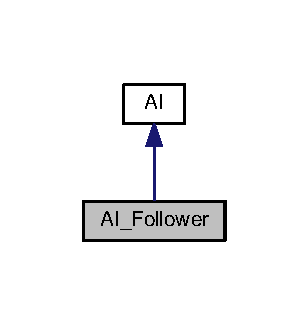
\includegraphics[width=148pt]{class_a_i___follower__inherit__graph}
\end{center}
\end{figure}


Collaboration diagram for A\+I\+\_\+\+Follower\+:
\nopagebreak
\begin{figure}[H]
\begin{center}
\leavevmode
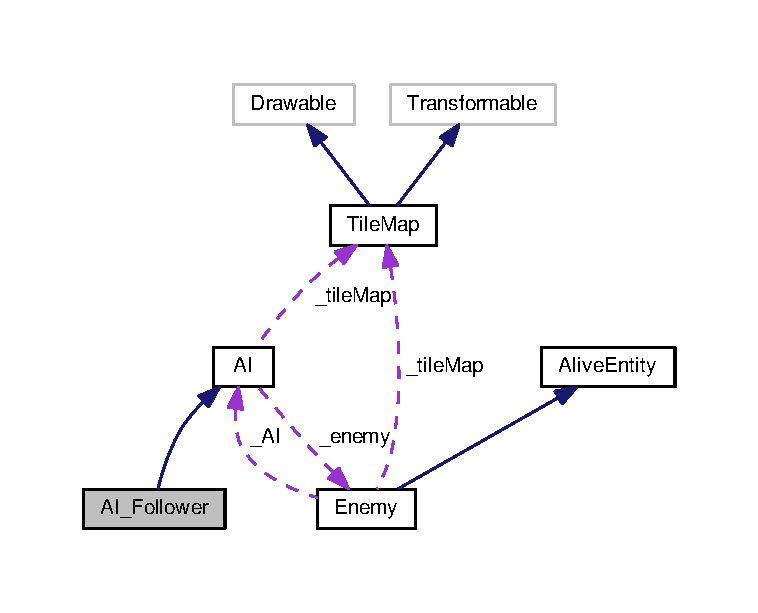
\includegraphics[width=350pt]{class_a_i___follower__coll__graph}
\end{center}
\end{figure}
\subsection*{Public Member Functions}
\begin{DoxyCompactItemize}
\item 
\hyperlink{class_a_i___follower_a3f1b82aaaffd50eb7a4d7340e376f52b}{A\+I\+\_\+\+Follower} (\hyperlink{class_jumper}{Jumper} $\ast$follower, const \hyperlink{class_tile_map}{Tile\+Map} \&tilemap, const \hyperlink{class_personnage}{Personnage} \&p)
\begin{DoxyCompactList}\small\item\em Constructeur de l'I\+A follower. \end{DoxyCompactList}\item 
virtual void \hyperlink{class_a_i___follower_a37893e7aa601169682333af093235c13}{move} ()
\begin{DoxyCompactList}\small\item\em Procédure gérant le mouvement de l'ennemi. \end{DoxyCompactList}\end{DoxyCompactItemize}
\subsection*{Additional Inherited Members}


\subsection{Detailed Description}
Classe gérant l'\hyperlink{class_a_i}{A\+I} des ennemi qui sautent. 

\subsection{Constructor \& Destructor Documentation}
\hypertarget{class_a_i___follower_a3f1b82aaaffd50eb7a4d7340e376f52b}{\index{A\+I\+\_\+\+Follower@{A\+I\+\_\+\+Follower}!A\+I\+\_\+\+Follower@{A\+I\+\_\+\+Follower}}
\index{A\+I\+\_\+\+Follower@{A\+I\+\_\+\+Follower}!A\+I\+\_\+\+Follower@{A\+I\+\_\+\+Follower}}
\subsubsection[{A\+I\+\_\+\+Follower}]{\setlength{\rightskip}{0pt plus 5cm}A\+I\+\_\+\+Follower\+::\+A\+I\+\_\+\+Follower (
\begin{DoxyParamCaption}
\item[{{\bf Jumper} $\ast$}]{follower, }
\item[{const {\bf Tile\+Map} \&}]{tilemap, }
\item[{const {\bf Personnage} \&}]{p}
\end{DoxyParamCaption}
)}}\label{class_a_i___follower_a3f1b82aaaffd50eb7a4d7340e376f52b}


Constructeur de l'I\+A follower. 

Constructeur de l'I\+A follower


\begin{DoxyParams}{Parameters}
{\em follower} & Pointeur vers l'ennemi \\
\hline
{\em tilemap} & La tile\+Map sur laquelle est l'ennemi \\
\hline
{\em p} & Le personnage à suivre \\
\hline
\end{DoxyParams}


\subsection{Member Function Documentation}
\hypertarget{class_a_i___follower_a37893e7aa601169682333af093235c13}{\index{A\+I\+\_\+\+Follower@{A\+I\+\_\+\+Follower}!move@{move}}
\index{move@{move}!A\+I\+\_\+\+Follower@{A\+I\+\_\+\+Follower}}
\subsubsection[{move}]{\setlength{\rightskip}{0pt plus 5cm}void A\+I\+\_\+\+Follower\+::move (
\begin{DoxyParamCaption}
{}
\end{DoxyParamCaption}
)\hspace{0.3cm}{\ttfamily [virtual]}}}\label{class_a_i___follower_a37893e7aa601169682333af093235c13}


Procédure gérant le mouvement de l'ennemi. 

Procédure qui permet de mouvoir l'ennemi en fonction de l'\hyperlink{class_a_i}{A\+I} qu'il a adopter 

Implements \hyperlink{class_a_i_a029ec0ca07e6644af6662cf08300ed0c}{A\+I}.



The documentation for this class was generated from the following file\+:\begin{DoxyCompactItemize}
\item 
\hyperlink{_a_i___follower_8hpp}{A\+I\+\_\+\+Follower.\+hpp}\end{DoxyCompactItemize}

\hypertarget{class_a_i___jumper}{\section{A\+I\+\_\+\+Jumper Class Reference}
\label{class_a_i___jumper}\index{A\+I\+\_\+\+Jumper@{A\+I\+\_\+\+Jumper}}
}


Classe gérant l'\hyperlink{class_a_i}{A\+I} des ennemi qui sautent.  




{\ttfamily \#include $<$A\+I\+\_\+\+Jumper.\+hpp$>$}



Inheritance diagram for A\+I\+\_\+\+Jumper\+:
\nopagebreak
\begin{figure}[H]
\begin{center}
\leavevmode
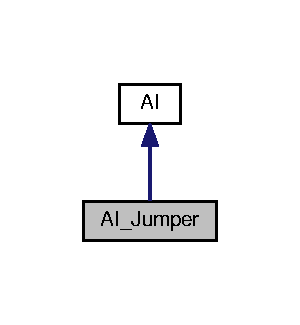
\includegraphics[width=144pt]{class_a_i___jumper__inherit__graph}
\end{center}
\end{figure}


Collaboration diagram for A\+I\+\_\+\+Jumper\+:
\nopagebreak
\begin{figure}[H]
\begin{center}
\leavevmode
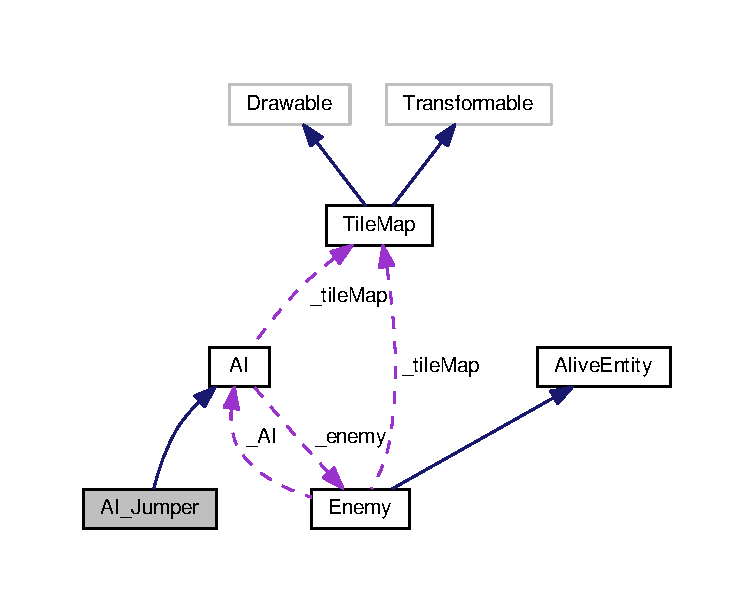
\includegraphics[width=350pt]{class_a_i___jumper__coll__graph}
\end{center}
\end{figure}
\subsection*{Public Member Functions}
\begin{DoxyCompactItemize}
\item 
\hyperlink{class_a_i___jumper_ad7af924ab722f5d4647fb0913dcc078f}{A\+I\+\_\+\+Jumper} (\hyperlink{class_jumper}{Jumper} $\ast$jumper, const \hyperlink{class_tile_map}{Tile\+Map} \&tilemap)
\begin{DoxyCompactList}\small\item\em Constructeur. \end{DoxyCompactList}\item 
virtual void \hyperlink{class_a_i___jumper_a49e2ba05ef7f14020faf4f521370dbfa}{move} ()
\begin{DoxyCompactList}\small\item\em Procédure gérant le mouvement de l'ennemi. \end{DoxyCompactList}\end{DoxyCompactItemize}
\subsection*{Additional Inherited Members}


\subsection{Detailed Description}
Classe gérant l'\hyperlink{class_a_i}{A\+I} des ennemi qui sautent. 

\subsection{Constructor \& Destructor Documentation}
\hypertarget{class_a_i___jumper_ad7af924ab722f5d4647fb0913dcc078f}{\index{A\+I\+\_\+\+Jumper@{A\+I\+\_\+\+Jumper}!A\+I\+\_\+\+Jumper@{A\+I\+\_\+\+Jumper}}
\index{A\+I\+\_\+\+Jumper@{A\+I\+\_\+\+Jumper}!A\+I\+\_\+\+Jumper@{A\+I\+\_\+\+Jumper}}
\subsubsection[{A\+I\+\_\+\+Jumper}]{\setlength{\rightskip}{0pt plus 5cm}A\+I\+\_\+\+Jumper\+::\+A\+I\+\_\+\+Jumper (
\begin{DoxyParamCaption}
\item[{{\bf Jumper} $\ast$}]{jumper, }
\item[{const {\bf Tile\+Map} \&}]{tilemap}
\end{DoxyParamCaption}
)}}\label{class_a_i___jumper_ad7af924ab722f5d4647fb0913dcc078f}


Constructeur. 

Constructeur de la classe \hyperlink{class_a_i___jumper}{A\+I\+\_\+\+Jumper}.


\begin{DoxyParams}{Parameters}
{\em enemy} & \+: Ennemi utilisant l'I\+A, tilemap \+: \hyperlink{class_tile_map}{Tile\+Map} sur laquelle l'\hyperlink{class_enemy}{Enemy} est. \\
\hline
\end{DoxyParams}


\subsection{Member Function Documentation}
\hypertarget{class_a_i___jumper_a49e2ba05ef7f14020faf4f521370dbfa}{\index{A\+I\+\_\+\+Jumper@{A\+I\+\_\+\+Jumper}!move@{move}}
\index{move@{move}!A\+I\+\_\+\+Jumper@{A\+I\+\_\+\+Jumper}}
\subsubsection[{move}]{\setlength{\rightskip}{0pt plus 5cm}void A\+I\+\_\+\+Jumper\+::move (
\begin{DoxyParamCaption}
{}
\end{DoxyParamCaption}
)\hspace{0.3cm}{\ttfamily [virtual]}}}\label{class_a_i___jumper_a49e2ba05ef7f14020faf4f521370dbfa}


Procédure gérant le mouvement de l'ennemi. 

Procédure qui permet de mouvoir l'ennemi en fonction de l'\hyperlink{class_a_i}{A\+I} qu'il a adopter 

Implements \hyperlink{class_a_i_a029ec0ca07e6644af6662cf08300ed0c}{A\+I}.



The documentation for this class was generated from the following file\+:\begin{DoxyCompactItemize}
\item 
\hyperlink{_a_i___jumper_8hpp}{A\+I\+\_\+\+Jumper.\+hpp}\end{DoxyCompactItemize}

\hypertarget{class_a_i___land_base}{\section{A\+I\+\_\+\+Land\+Base Class Reference}
\label{class_a_i___land_base}\index{A\+I\+\_\+\+Land\+Base@{A\+I\+\_\+\+Land\+Base}}
}


Classe gérant l'\hyperlink{class_a_i}{A\+I} des ennemi qui marchent.  




{\ttfamily \#include $<$A\+I\+\_\+\+Land\+Base.\+hpp$>$}



Inheritance diagram for A\+I\+\_\+\+Land\+Base\+:
\nopagebreak
\begin{figure}[H]
\begin{center}
\leavevmode
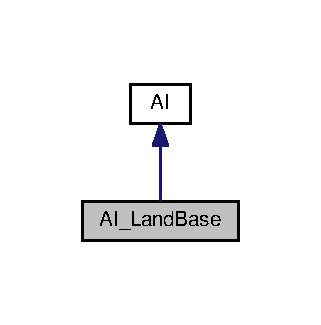
\includegraphics[width=154pt]{class_a_i___land_base__inherit__graph}
\end{center}
\end{figure}


Collaboration diagram for A\+I\+\_\+\+Land\+Base\+:
\nopagebreak
\begin{figure}[H]
\begin{center}
\leavevmode
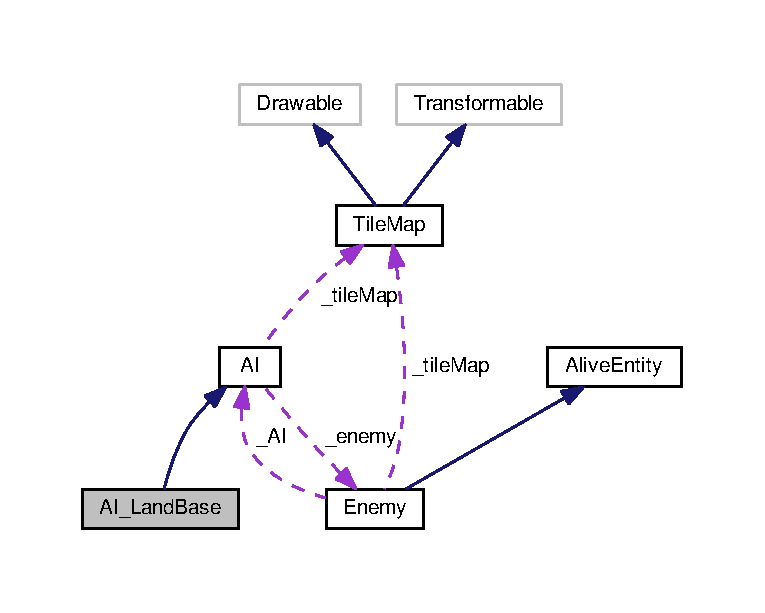
\includegraphics[width=350pt]{class_a_i___land_base__coll__graph}
\end{center}
\end{figure}
\subsection*{Public Member Functions}
\begin{DoxyCompactItemize}
\item 
\hyperlink{class_a_i___land_base_aefdd3e725dfa9cffda076c6ee268342f}{A\+I\+\_\+\+Land\+Base} (\hyperlink{class_enemy}{Enemy} $\ast$enemy, const \hyperlink{class_tile_map}{Tile\+Map} \&tilemap)
\begin{DoxyCompactList}\small\item\em Constructeur. \end{DoxyCompactList}\item 
virtual void \hyperlink{class_a_i___land_base_af536a9f2a45fd52189542761bcf285d4}{move} ()
\begin{DoxyCompactList}\small\item\em Procédure gérant le mouvement de l'ennemi. \end{DoxyCompactList}\end{DoxyCompactItemize}
\subsection*{Additional Inherited Members}


\subsection{Detailed Description}
Classe gérant l'\hyperlink{class_a_i}{A\+I} des ennemi qui marchent. 

\subsection{Constructor \& Destructor Documentation}
\hypertarget{class_a_i___land_base_aefdd3e725dfa9cffda076c6ee268342f}{\index{A\+I\+\_\+\+Land\+Base@{A\+I\+\_\+\+Land\+Base}!A\+I\+\_\+\+Land\+Base@{A\+I\+\_\+\+Land\+Base}}
\index{A\+I\+\_\+\+Land\+Base@{A\+I\+\_\+\+Land\+Base}!A\+I\+\_\+\+Land\+Base@{A\+I\+\_\+\+Land\+Base}}
\subsubsection[{A\+I\+\_\+\+Land\+Base}]{\setlength{\rightskip}{0pt plus 5cm}A\+I\+\_\+\+Land\+Base\+::\+A\+I\+\_\+\+Land\+Base (
\begin{DoxyParamCaption}
\item[{{\bf Enemy} $\ast$}]{enemy, }
\item[{const {\bf Tile\+Map} \&}]{tilemap}
\end{DoxyParamCaption}
)}}\label{class_a_i___land_base_aefdd3e725dfa9cffda076c6ee268342f}


Constructeur. 

Constructeur de la classe A\+I\+\_\+\+Jump\+Random.


\begin{DoxyParams}{Parameters}
{\em enemy} & \+: Ennemi utilisant l'I\+A, tilemap \+: \hyperlink{class_tile_map}{Tile\+Map} sur laquelle l'\hyperlink{class_enemy}{Enemy} est. \\
\hline
\end{DoxyParams}


\subsection{Member Function Documentation}
\hypertarget{class_a_i___land_base_af536a9f2a45fd52189542761bcf285d4}{\index{A\+I\+\_\+\+Land\+Base@{A\+I\+\_\+\+Land\+Base}!move@{move}}
\index{move@{move}!A\+I\+\_\+\+Land\+Base@{A\+I\+\_\+\+Land\+Base}}
\subsubsection[{move}]{\setlength{\rightskip}{0pt plus 5cm}void A\+I\+\_\+\+Land\+Base\+::move (
\begin{DoxyParamCaption}
{}
\end{DoxyParamCaption}
)\hspace{0.3cm}{\ttfamily [virtual]}}}\label{class_a_i___land_base_af536a9f2a45fd52189542761bcf285d4}


Procédure gérant le mouvement de l'ennemi. 

Procédure qui permet de mouvoir l'ennemi en fonction de l'\hyperlink{class_a_i}{A\+I} qu'il a adopter 

Implements \hyperlink{class_a_i_a029ec0ca07e6644af6662cf08300ed0c}{A\+I}.



The documentation for this class was generated from the following file\+:\begin{DoxyCompactItemize}
\item 
\hyperlink{_a_i___land_base_8hpp}{A\+I\+\_\+\+Land\+Base.\+hpp}\end{DoxyCompactItemize}

\hypertarget{class_alive_entity}{\section{Alive\+Entity Class Reference}
\label{class_alive_entity}\index{Alive\+Entity@{Alive\+Entity}}
}


Classe abstraite qui définissant les objets \char`\"{}vivants\char`\"{}.  




{\ttfamily \#include $<$Alive\+Entity.\+hpp$>$}



Inheritance diagram for Alive\+Entity\+:
\nopagebreak
\begin{figure}[H]
\begin{center}
\leavevmode
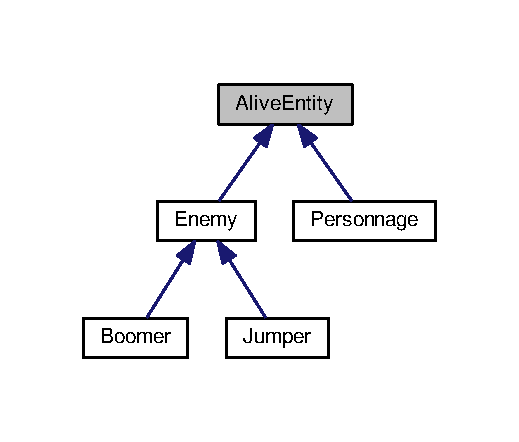
\includegraphics[width=249pt]{class_alive_entity__inherit__graph}
\end{center}
\end{figure}
\subsection*{Public Member Functions}
\begin{DoxyCompactItemize}
\item 
\hyperlink{class_alive_entity_a67bebe6bcef18c0989208060da3b13b2}{Alive\+Entity} (const sf\+::\+Vector2f \&taille)
\begin{DoxyCompactList}\small\item\em Constructeur. \end{DoxyCompactList}\item 
sf\+::\+Vector2f \hyperlink{class_alive_entity_ae90ba96bdca3921e66508753a281fd08}{get\+Mouvement} () const 
\begin{DoxyCompactList}\small\item\em Getter du Mouvement de l'entité. \end{DoxyCompactList}\item 
void \hyperlink{class_alive_entity_af4c6753b36371340afaaae76a5bed7ee}{set\+Mouvement} (sf\+::\+Vector2f v)
\begin{DoxyCompactList}\small\item\em Setter du Mouvement de l'entité. \end{DoxyCompactList}\item 
void \hyperlink{class_alive_entity_aabfbf6895cde97b0ef8d50267ade8970}{add\+Mouvement} (const sf\+::\+Vector2f \&mvt)
\begin{DoxyCompactList}\small\item\em Incrémente le mouvement de l'objet. \end{DoxyCompactList}\item 
void \hyperlink{class_alive_entity_aaca9b5defd187382991876ae32de6779}{add\+Mouvement} (float x, float y)
\begin{DoxyCompactList}\small\item\em Incrémente le mouvement de l'objet. \end{DoxyCompactList}\item 
sf\+::\+Rectangle\+Shape \hyperlink{class_alive_entity_a6f795a340c1842a39bfbe16d3997cd91}{get\+Shape} () const 
\begin{DoxyCompactList}\small\item\em Getter de la Rectangle\+Shape de l'entité. \end{DoxyCompactList}\item 
void \hyperlink{class_alive_entity_a04ae0cdbba3ebcfe08c7dd6eda09dd00}{set\+Position} (sf\+::\+Vector2f v)
\begin{DoxyCompactList}\small\item\em Setter de la position. \end{DoxyCompactList}\item 
void \hyperlink{class_alive_entity_a33f720218560af101a2a4ab040ad02d8}{set\+Position} (float x, float y)
\begin{DoxyCompactList}\small\item\em Setter de la position. \end{DoxyCompactList}\item 
void \hyperlink{class_alive_entity_acd80dd8cf81e081cf0369b3e20d45788}{set\+Size} (float x, float y)
\begin{DoxyCompactList}\small\item\em Setter de la taille. \end{DoxyCompactList}\item 
const sf\+::\+Vector2f \& \hyperlink{class_alive_entity_ac4d5ac19490963c25a49b07a2f6adfd9}{get\+Position} () const 
\begin{DoxyCompactList}\small\item\em Getter de la position. \end{DoxyCompactList}\item 
const sf\+::\+Vector2f \& \hyperlink{class_alive_entity_a5560db2181eefaf88d4fbf9410cfc96f}{get\+Size} () const 
\begin{DoxyCompactList}\small\item\em Getter de la Size. \end{DoxyCompactList}\end{DoxyCompactItemize}
\subsection*{Protected Attributes}
\begin{DoxyCompactItemize}
\item 
\hypertarget{class_alive_entity_ab7518854489cbe9ea8d057168caf9c5a}{sf\+::\+Vector2f {\bfseries \+\_\+mouvement}}\label{class_alive_entity_ab7518854489cbe9ea8d057168caf9c5a}

\item 
sf\+::\+Rectangle\+Shape \hyperlink{class_alive_entity_a0de4bf929f42b7a090c09d8805953128}{\+\_\+shape}
\end{DoxyCompactItemize}


\subsection{Detailed Description}
Classe abstraite qui définissant les objets \char`\"{}vivants\char`\"{}. 

Classe abstraite qui définit les méthodes des \hyperlink{class_enemy}{Enemy} et du \hyperlink{class_personnage}{Personnage}. 

\subsection{Constructor \& Destructor Documentation}
\hypertarget{class_alive_entity_a67bebe6bcef18c0989208060da3b13b2}{\index{Alive\+Entity@{Alive\+Entity}!Alive\+Entity@{Alive\+Entity}}
\index{Alive\+Entity@{Alive\+Entity}!Alive\+Entity@{Alive\+Entity}}
\subsubsection[{Alive\+Entity}]{\setlength{\rightskip}{0pt plus 5cm}Alive\+Entity\+::\+Alive\+Entity (
\begin{DoxyParamCaption}
\item[{const sf\+::\+Vector2f \&}]{taille}
\end{DoxyParamCaption}
)}}\label{class_alive_entity_a67bebe6bcef18c0989208060da3b13b2}


Constructeur. 

Constructeur de la classe \hyperlink{class_alive_entity}{Alive\+Entity}


\begin{DoxyParams}{Parameters}
{\em taille} & \+: taille de l'objet. \\
\hline
\end{DoxyParams}


\subsection{Member Function Documentation}
\hypertarget{class_alive_entity_aabfbf6895cde97b0ef8d50267ade8970}{\index{Alive\+Entity@{Alive\+Entity}!add\+Mouvement@{add\+Mouvement}}
\index{add\+Mouvement@{add\+Mouvement}!Alive\+Entity@{Alive\+Entity}}
\subsubsection[{add\+Mouvement}]{\setlength{\rightskip}{0pt plus 5cm}void Alive\+Entity\+::add\+Mouvement (
\begin{DoxyParamCaption}
\item[{const sf\+::\+Vector2f \&}]{mvt}
\end{DoxyParamCaption}
)}}\label{class_alive_entity_aabfbf6895cde97b0ef8d50267ade8970}


Incrémente le mouvement de l'objet. 

Ajoute au vector déjà existant un nouveau mouvement.


\begin{DoxyParams}{Parameters}
{\em mvt} & \+: mouvement à ajouter. \\
\hline
\end{DoxyParams}
\hypertarget{class_alive_entity_aaca9b5defd187382991876ae32de6779}{\index{Alive\+Entity@{Alive\+Entity}!add\+Mouvement@{add\+Mouvement}}
\index{add\+Mouvement@{add\+Mouvement}!Alive\+Entity@{Alive\+Entity}}
\subsubsection[{add\+Mouvement}]{\setlength{\rightskip}{0pt plus 5cm}void Alive\+Entity\+::add\+Mouvement (
\begin{DoxyParamCaption}
\item[{float}]{x, }
\item[{float}]{y}
\end{DoxyParamCaption}
)}}\label{class_alive_entity_aaca9b5defd187382991876ae32de6779}


Incrémente le mouvement de l'objet. 

Ajoute au vector déjà existant un nouveau mouvement.


\begin{DoxyParams}{Parameters}
{\em x} & \+: mouvement en x, y \+: mouvement en y. \\
\hline
\end{DoxyParams}
\hypertarget{class_alive_entity_ae90ba96bdca3921e66508753a281fd08}{\index{Alive\+Entity@{Alive\+Entity}!get\+Mouvement@{get\+Mouvement}}
\index{get\+Mouvement@{get\+Mouvement}!Alive\+Entity@{Alive\+Entity}}
\subsubsection[{get\+Mouvement}]{\setlength{\rightskip}{0pt plus 5cm}sf\+::\+Vector2f Alive\+Entity\+::get\+Mouvement (
\begin{DoxyParamCaption}
{}
\end{DoxyParamCaption}
) const}}\label{class_alive_entity_ae90ba96bdca3921e66508753a281fd08}


Getter du Mouvement de l'entité. 

Fonction retournant le prochain déplacement de x et en y de l'entité.

\begin{DoxyReturn}{Returns}
Un Vector2f équivalent au prochain mouvement de l'entité 
\end{DoxyReturn}
\hypertarget{class_alive_entity_ac4d5ac19490963c25a49b07a2f6adfd9}{\index{Alive\+Entity@{Alive\+Entity}!get\+Position@{get\+Position}}
\index{get\+Position@{get\+Position}!Alive\+Entity@{Alive\+Entity}}
\subsubsection[{get\+Position}]{\setlength{\rightskip}{0pt plus 5cm}const sf\+::\+Vector2f \& Alive\+Entity\+::get\+Position (
\begin{DoxyParamCaption}
{}
\end{DoxyParamCaption}
) const}}\label{class_alive_entity_ac4d5ac19490963c25a49b07a2f6adfd9}


Getter de la position. 

Récupère la position de l'objet

\begin{DoxyReturn}{Returns}
Vector2f équivalent à la position de l'objet 
\end{DoxyReturn}
\hypertarget{class_alive_entity_a6f795a340c1842a39bfbe16d3997cd91}{\index{Alive\+Entity@{Alive\+Entity}!get\+Shape@{get\+Shape}}
\index{get\+Shape@{get\+Shape}!Alive\+Entity@{Alive\+Entity}}
\subsubsection[{get\+Shape}]{\setlength{\rightskip}{0pt plus 5cm}sf\+::\+Rectangle\+Shape Alive\+Entity\+::get\+Shape (
\begin{DoxyParamCaption}
{}
\end{DoxyParamCaption}
) const}}\label{class_alive_entity_a6f795a340c1842a39bfbe16d3997cd91}


Getter de la Rectangle\+Shape de l'entité. 

Récupère le rectangle correspondant à la taille de l'objet (contour) Utile notamment pour les collisions/déplacements.

\begin{DoxyReturn}{Returns}
La Rectangle\+Shape de l'objet 
\end{DoxyReturn}
\hypertarget{class_alive_entity_a5560db2181eefaf88d4fbf9410cfc96f}{\index{Alive\+Entity@{Alive\+Entity}!get\+Size@{get\+Size}}
\index{get\+Size@{get\+Size}!Alive\+Entity@{Alive\+Entity}}
\subsubsection[{get\+Size}]{\setlength{\rightskip}{0pt plus 5cm}const sf\+::\+Vector2f \& Alive\+Entity\+::get\+Size (
\begin{DoxyParamCaption}
{}
\end{DoxyParamCaption}
) const}}\label{class_alive_entity_a5560db2181eefaf88d4fbf9410cfc96f}


Getter de la Size. 

Récupère la taille de l'objet

\begin{DoxyReturn}{Returns}
Vector2f équivalent à la taille de l'objet 
\end{DoxyReturn}
\hypertarget{class_alive_entity_af4c6753b36371340afaaae76a5bed7ee}{\index{Alive\+Entity@{Alive\+Entity}!set\+Mouvement@{set\+Mouvement}}
\index{set\+Mouvement@{set\+Mouvement}!Alive\+Entity@{Alive\+Entity}}
\subsubsection[{set\+Mouvement}]{\setlength{\rightskip}{0pt plus 5cm}void Alive\+Entity\+::set\+Mouvement (
\begin{DoxyParamCaption}
\item[{sf\+::\+Vector2f}]{v}
\end{DoxyParamCaption}
)}}\label{class_alive_entity_af4c6753b36371340afaaae76a5bed7ee}


Setter du Mouvement de l'entité. 

Méthode permettant de donner un mouvement défini (2\+D) à un objet.


\begin{DoxyParams}{Parameters}
{\em v} & \+: vecteur 2 dimensions qui définira le nouveau mouvement \\
\hline
\end{DoxyParams}
\hypertarget{class_alive_entity_a04ae0cdbba3ebcfe08c7dd6eda09dd00}{\index{Alive\+Entity@{Alive\+Entity}!set\+Position@{set\+Position}}
\index{set\+Position@{set\+Position}!Alive\+Entity@{Alive\+Entity}}
\subsubsection[{set\+Position}]{\setlength{\rightskip}{0pt plus 5cm}void Alive\+Entity\+::set\+Position (
\begin{DoxyParamCaption}
\item[{sf\+::\+Vector2f}]{v}
\end{DoxyParamCaption}
)}}\label{class_alive_entity_a04ae0cdbba3ebcfe08c7dd6eda09dd00}


Setter de la position. 

Initialiste la position de l'objet.


\begin{DoxyParams}{Parameters}
{\em v} & \+: Vector correspondant aux coordonnées. \\
\hline
\end{DoxyParams}
\hypertarget{class_alive_entity_a33f720218560af101a2a4ab040ad02d8}{\index{Alive\+Entity@{Alive\+Entity}!set\+Position@{set\+Position}}
\index{set\+Position@{set\+Position}!Alive\+Entity@{Alive\+Entity}}
\subsubsection[{set\+Position}]{\setlength{\rightskip}{0pt plus 5cm}void Alive\+Entity\+::set\+Position (
\begin{DoxyParamCaption}
\item[{float}]{x, }
\item[{float}]{y}
\end{DoxyParamCaption}
)}}\label{class_alive_entity_a33f720218560af101a2a4ab040ad02d8}


Setter de la position. 

Initialiste la position de l'objet.


\begin{DoxyParams}{Parameters}
{\em x} & \+: coordonnée en x, y \+: coordonnée en y. \\
\hline
\end{DoxyParams}
\hypertarget{class_alive_entity_acd80dd8cf81e081cf0369b3e20d45788}{\index{Alive\+Entity@{Alive\+Entity}!set\+Size@{set\+Size}}
\index{set\+Size@{set\+Size}!Alive\+Entity@{Alive\+Entity}}
\subsubsection[{set\+Size}]{\setlength{\rightskip}{0pt plus 5cm}void Alive\+Entity\+::set\+Size (
\begin{DoxyParamCaption}
\item[{float}]{x, }
\item[{float}]{y}
\end{DoxyParamCaption}
)}}\label{class_alive_entity_acd80dd8cf81e081cf0369b3e20d45788}


Setter de la taille. 

Setter de la taille


\begin{DoxyParams}{Parameters}
{\em x} & Nouvelle taille en x \\
\hline
{\em y} & Nouvelle taille en y \\
\hline
\end{DoxyParams}


\subsection{Member Data Documentation}
\hypertarget{class_alive_entity_a0de4bf929f42b7a090c09d8805953128}{\index{Alive\+Entity@{Alive\+Entity}!\+\_\+shape@{\+\_\+shape}}
\index{\+\_\+shape@{\+\_\+shape}!Alive\+Entity@{Alive\+Entity}}
\subsubsection[{\+\_\+shape}]{\setlength{\rightskip}{0pt plus 5cm}sf\+::\+Rectangle\+Shape Alive\+Entity\+::\+\_\+shape\hspace{0.3cm}{\ttfamily [protected]}}}\label{class_alive_entity_a0de4bf929f42b7a090c09d8805953128}
Prochain mouvement 

The documentation for this class was generated from the following file\+:\begin{DoxyCompactItemize}
\item 
\hyperlink{_alive_entity_8hpp}{Alive\+Entity.\+hpp}\end{DoxyCompactItemize}

\hypertarget{class_boomer}{\section{Boomer Class Reference}
\label{class_boomer}\index{Boomer@{Boomer}}
}


Classe gérant les ennemi qui explosent et se devisent.  




{\ttfamily \#include $<$Boomer.\+hpp$>$}



Inheritance diagram for Boomer\+:
\nopagebreak
\begin{figure}[H]
\begin{center}
\leavevmode
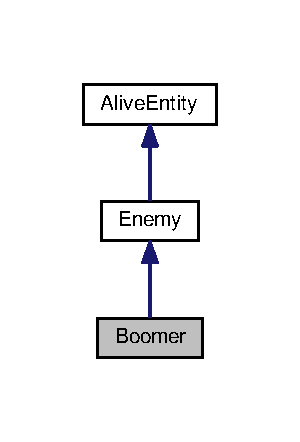
\includegraphics[width=144pt]{class_boomer__inherit__graph}
\end{center}
\end{figure}


Collaboration diagram for Boomer\+:
\nopagebreak
\begin{figure}[H]
\begin{center}
\leavevmode
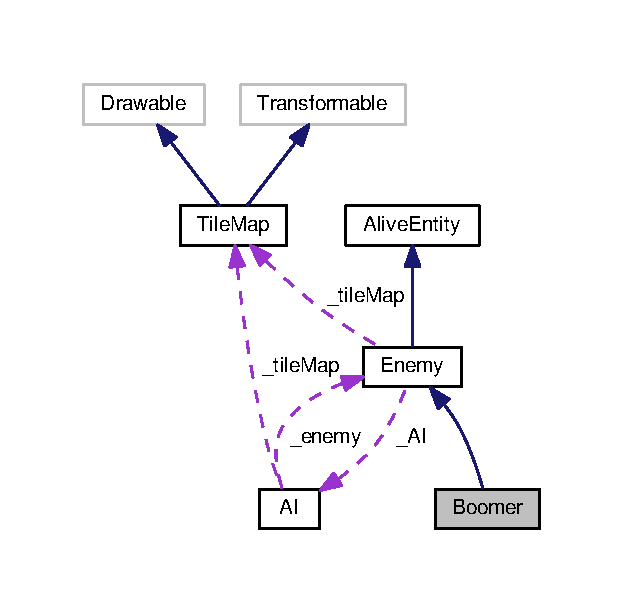
\includegraphics[width=299pt]{class_boomer__coll__graph}
\end{center}
\end{figure}
\subsection*{Public Member Functions}
\begin{DoxyCompactItemize}
\item 
\hyperlink{class_boomer_a45e535e25b46f8ae440a929bf7c2dddd}{Boomer} (const sf\+::\+Vector2f \&taille, \hyperlink{class_tile_map}{Tile\+Map} \&tilemap, int fat\+Per\+Frame, \hyperlink{class_enemy}{Enemy} $\ast$prototype)
\begin{DoxyCompactList}\small\item\em Constructeur du \hyperlink{class_boomer}{Boomer}. \end{DoxyCompactList}\item 
\hyperlink{class_enemy}{Enemy} $\ast$ \hyperlink{class_boomer_a757fb2c73fad3ab04086b9bbb15208b0}{clone} ()
\begin{DoxyCompactList}\small\item\em Clone le \hyperlink{class_boomer}{Boomer}. \end{DoxyCompactList}\item 
unsigned int \hyperlink{class_boomer_a8fa91ac287ca7f7cfd9f1cf1ce154870}{get\+Fat\+Per\+Frame} () const 
\begin{DoxyCompactList}\small\item\em Getter du grossissement par frame. \end{DoxyCompactList}\item 
void \hyperlink{class_boomer_a30a5e9732c86abc616a6d31badbb2ce8}{jump\+On} ()
\begin{DoxyCompactList}\small\item\em Actions à faire si on saute sur l'ennemi. \end{DoxyCompactList}\end{DoxyCompactItemize}
\subsection*{Additional Inherited Members}


\subsection{Detailed Description}
Classe gérant les ennemi qui explosent et se devisent. 

\subsection{Constructor \& Destructor Documentation}
\hypertarget{class_boomer_a45e535e25b46f8ae440a929bf7c2dddd}{\index{Boomer@{Boomer}!Boomer@{Boomer}}
\index{Boomer@{Boomer}!Boomer@{Boomer}}
\subsubsection[{Boomer}]{\setlength{\rightskip}{0pt plus 5cm}Boomer\+::\+Boomer (
\begin{DoxyParamCaption}
\item[{const sf\+::\+Vector2f \&}]{taille, }
\item[{{\bf Tile\+Map} \&}]{tilemap, }
\item[{int}]{fat\+Per\+Frame, }
\item[{{\bf Enemy} $\ast$}]{prototype}
\end{DoxyParamCaption}
)}}\label{class_boomer_a45e535e25b46f8ae440a929bf7c2dddd}


Constructeur du \hyperlink{class_boomer}{Boomer}. 

Constructeur du \hyperlink{class_boomer}{Boomer}


\begin{DoxyParams}{Parameters}
{\em taille} & Taille de la hitbox \\
\hline
{\em tilemap} & Map sur laquelle est l'ennemi \\
\hline
{\em grossissement} & par frame \\
\hline
{\em l'ennemi} & qui sortiera une fois le boomer tué \\
\hline
\end{DoxyParams}


\subsection{Member Function Documentation}
\hypertarget{class_boomer_a757fb2c73fad3ab04086b9bbb15208b0}{\index{Boomer@{Boomer}!clone@{clone}}
\index{clone@{clone}!Boomer@{Boomer}}
\subsubsection[{clone}]{\setlength{\rightskip}{0pt plus 5cm}{\bf Enemy} $\ast$ Boomer\+::clone (
\begin{DoxyParamCaption}
{}
\end{DoxyParamCaption}
)\hspace{0.3cm}{\ttfamily [virtual]}}}\label{class_boomer_a757fb2c73fad3ab04086b9bbb15208b0}


Clone le \hyperlink{class_boomer}{Boomer}. 

Créer un nouveau \hyperlink{class_boomer}{Boomer} avec les même caractéristiques.

\begin{DoxyReturn}{Returns}
Un clone du \hyperlink{class_boomer}{Boomer} existant 
\end{DoxyReturn}


Implements \hyperlink{class_enemy_a21d5d2f97aa7406a985fd0ca3f3b1028}{Enemy}.

\hypertarget{class_boomer_a8fa91ac287ca7f7cfd9f1cf1ce154870}{\index{Boomer@{Boomer}!get\+Fat\+Per\+Frame@{get\+Fat\+Per\+Frame}}
\index{get\+Fat\+Per\+Frame@{get\+Fat\+Per\+Frame}!Boomer@{Boomer}}
\subsubsection[{get\+Fat\+Per\+Frame}]{\setlength{\rightskip}{0pt plus 5cm}unsigned int Boomer\+::get\+Fat\+Per\+Frame (
\begin{DoxyParamCaption}
{}
\end{DoxyParamCaption}
) const}}\label{class_boomer_a8fa91ac287ca7f7cfd9f1cf1ce154870}


Getter du grossissement par frame. 

Getter de grossissement par frame \begin{DoxyReturn}{Returns}
Retourne la valeure du grossissement par frame 
\end{DoxyReturn}
\hypertarget{class_boomer_a30a5e9732c86abc616a6d31badbb2ce8}{\index{Boomer@{Boomer}!jump\+On@{jump\+On}}
\index{jump\+On@{jump\+On}!Boomer@{Boomer}}
\subsubsection[{jump\+On}]{\setlength{\rightskip}{0pt plus 5cm}void Boomer\+::jump\+On (
\begin{DoxyParamCaption}
{}
\end{DoxyParamCaption}
)\hspace{0.3cm}{\ttfamily [virtual]}}}\label{class_boomer_a30a5e9732c86abc616a6d31badbb2ce8}


Actions à faire si on saute sur l'ennemi. 

Actions à faire si on saute sur l'ennemi 

Reimplemented from \hyperlink{class_enemy_a85c7ff8dc9f54c92d7583c0d196d37d2}{Enemy}.



The documentation for this class was generated from the following file\+:\begin{DoxyCompactItemize}
\item 
\hyperlink{_boomer_8hpp}{Boomer.\+hpp}\end{DoxyCompactItemize}

\hypertarget{class_enemy}{\section{Enemy Class Reference}
\label{class_enemy}\index{Enemy@{Enemy}}
}


Classe abstraite qui définissant les objets \char`\"{}vivants\char`\"{}.  




{\ttfamily \#include $<$Enemy.\+hpp$>$}



Inheritance diagram for Enemy\+:
\nopagebreak
\begin{figure}[H]
\begin{center}
\leavevmode
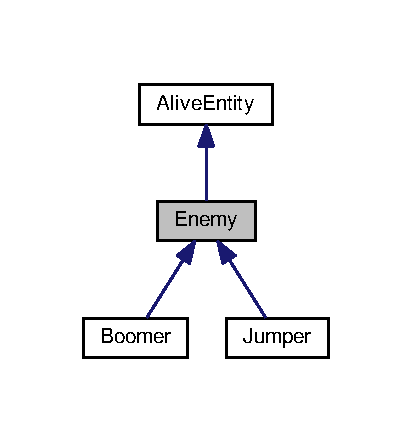
\includegraphics[width=197pt]{class_enemy__inherit__graph}
\end{center}
\end{figure}


Collaboration diagram for Enemy\+:
\nopagebreak
\begin{figure}[H]
\begin{center}
\leavevmode
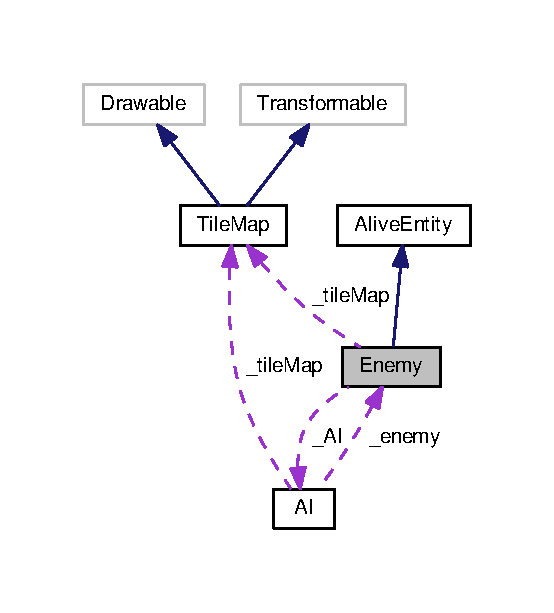
\includegraphics[width=266pt]{class_enemy__coll__graph}
\end{center}
\end{figure}
\subsection*{Public Member Functions}
\begin{DoxyCompactItemize}
\item 
\hyperlink{class_enemy_aa89c4b47d518fe6aa5e84b059b19a3b0}{Enemy} (const sf\+::\+Vector2f \&taille, \hyperlink{class_tile_map}{Tile\+Map} \&tilemap)
\begin{DoxyCompactList}\small\item\em Constructeur. \end{DoxyCompactList}\item 
virtual \hyperlink{class_enemy_a065a22a70c78bfc03da4c032312c6da5}{$\sim$\+Enemy} ()
\begin{DoxyCompactList}\small\item\em Destrcuteur. \end{DoxyCompactList}\item 
void \hyperlink{class_enemy_a9a398f8d12234f02563b27440aff7891}{move} ()
\begin{DoxyCompactList}\small\item\em Fonction bougeant l'ennemi. \end{DoxyCompactList}\item 
virtual \hyperlink{class_enemy}{Enemy} $\ast$ \hyperlink{class_enemy_a21d5d2f97aa7406a985fd0ca3f3b1028}{clone} ()=0
\begin{DoxyCompactList}\small\item\em Permet de clone l'ennemi (Pattern Prototype) \end{DoxyCompactList}\item 
virtual void \hyperlink{class_enemy_a85c7ff8dc9f54c92d7583c0d196d37d2}{jump\+On} ()
\begin{DoxyCompactList}\small\item\em Actions à faire si on saute sur l'ennemi. \end{DoxyCompactList}\item 
\hypertarget{class_enemy_a17fc0ab57aa01933301df1f7ced16b21}{virtual unsigned int {\bfseries get\+Reward} () const }\label{class_enemy_a17fc0ab57aa01933301df1f7ced16b21}

\end{DoxyCompactItemize}
\subsection*{Protected Attributes}
\begin{DoxyCompactItemize}
\item 
\hypertarget{class_enemy_a696bc97bd2f755fe2730d1a84602666b}{\hyperlink{class_a_i}{A\+I} $\ast$ {\bfseries \+\_\+\+A\+I}}\label{class_enemy_a696bc97bd2f755fe2730d1a84602666b}

\item 
\hyperlink{class_tile_map}{Tile\+Map} \& \hyperlink{class_enemy_a25c3a0c770a6cf5ae9cd9e4d71968aff}{\+\_\+tile\+Map}
\end{DoxyCompactItemize}


\subsection{Detailed Description}
Classe abstraite qui définissant les objets \char`\"{}vivants\char`\"{}. 

Classe définissant un ennemi. 

\subsection{Constructor \& Destructor Documentation}
\hypertarget{class_enemy_aa89c4b47d518fe6aa5e84b059b19a3b0}{\index{Enemy@{Enemy}!Enemy@{Enemy}}
\index{Enemy@{Enemy}!Enemy@{Enemy}}
\subsubsection[{Enemy}]{\setlength{\rightskip}{0pt plus 5cm}Enemy\+::\+Enemy (
\begin{DoxyParamCaption}
\item[{const sf\+::\+Vector2f \&}]{taille, }
\item[{{\bf Tile\+Map} \&}]{tilemap}
\end{DoxyParamCaption}
)}}\label{class_enemy_aa89c4b47d518fe6aa5e84b059b19a3b0}


Constructeur. 

Constructeur de la classe \hyperlink{class_enemy}{Enemy}


\begin{DoxyParams}{Parameters}
{\em taille} & \+: taille de l'objet, tilemap \+: \hyperlink{class_tile_map}{Tile\+Map} à laquelle l'ennemi est rattaché. \\
\hline
\end{DoxyParams}
\hypertarget{class_enemy_a065a22a70c78bfc03da4c032312c6da5}{\index{Enemy@{Enemy}!````~Enemy@{$\sim$\+Enemy}}
\index{````~Enemy@{$\sim$\+Enemy}!Enemy@{Enemy}}
\subsubsection[{$\sim$\+Enemy}]{\setlength{\rightskip}{0pt plus 5cm}virtual Enemy\+::$\sim$\+Enemy (
\begin{DoxyParamCaption}
{}
\end{DoxyParamCaption}
)\hspace{0.3cm}{\ttfamily [virtual]}}}\label{class_enemy_a065a22a70c78bfc03da4c032312c6da5}


Destrcuteur. 

Destructeur de la classe \hyperlink{class_enemy}{Enemy} 

\subsection{Member Function Documentation}
\hypertarget{class_enemy_a21d5d2f97aa7406a985fd0ca3f3b1028}{\index{Enemy@{Enemy}!clone@{clone}}
\index{clone@{clone}!Enemy@{Enemy}}
\subsubsection[{clone}]{\setlength{\rightskip}{0pt plus 5cm}{\bf Enemy} $\ast$ Enemy\+::clone (
\begin{DoxyParamCaption}
{}
\end{DoxyParamCaption}
)\hspace{0.3cm}{\ttfamily [pure virtual]}}}\label{class_enemy_a21d5d2f97aa7406a985fd0ca3f3b1028}


Permet de clone l'ennemi (Pattern Prototype) 

Permet de cloner un objet afin d'en instancier un certain nombre facilement.

\begin{DoxyReturn}{Returns}
Retourne un nouvel \hyperlink{class_enemy}{Enemy}. 
\end{DoxyReturn}


Implemented in \hyperlink{class_jumper_aa28b8e0acc2f4fa045b29359692fe4ac}{Jumper}, and \hyperlink{class_boomer_a757fb2c73fad3ab04086b9bbb15208b0}{Boomer}.

\hypertarget{class_enemy_a85c7ff8dc9f54c92d7583c0d196d37d2}{\index{Enemy@{Enemy}!jump\+On@{jump\+On}}
\index{jump\+On@{jump\+On}!Enemy@{Enemy}}
\subsubsection[{jump\+On}]{\setlength{\rightskip}{0pt plus 5cm}virtual void Enemy\+::jump\+On (
\begin{DoxyParamCaption}
{}
\end{DoxyParamCaption}
)\hspace{0.3cm}{\ttfamily [virtual]}}}\label{class_enemy_a85c7ff8dc9f54c92d7583c0d196d37d2}


Actions à faire si on saute sur l'ennemi. 

Actions à faire si on saute sur l'ennemi 

Reimplemented in \hyperlink{class_boomer_a30a5e9732c86abc616a6d31badbb2ce8}{Boomer}.

\hypertarget{class_enemy_a9a398f8d12234f02563b27440aff7891}{\index{Enemy@{Enemy}!move@{move}}
\index{move@{move}!Enemy@{Enemy}}
\subsubsection[{move}]{\setlength{\rightskip}{0pt plus 5cm}void Enemy\+::move (
\begin{DoxyParamCaption}
{}
\end{DoxyParamCaption}
)}}\label{class_enemy_a9a398f8d12234f02563b27440aff7891}


Fonction bougeant l'ennemi. 

Fonction utilisant le Pattern Strategy \hyperlink{class_a_i}{A\+I} pour mouvoir l'ennemi 

\subsection{Member Data Documentation}
\hypertarget{class_enemy_a25c3a0c770a6cf5ae9cd9e4d71968aff}{\index{Enemy@{Enemy}!\+\_\+tile\+Map@{\+\_\+tile\+Map}}
\index{\+\_\+tile\+Map@{\+\_\+tile\+Map}!Enemy@{Enemy}}
\subsubsection[{\+\_\+tile\+Map}]{\setlength{\rightskip}{0pt plus 5cm}{\bf Tile\+Map}\& Enemy\+::\+\_\+tile\+Map\hspace{0.3cm}{\ttfamily [protected]}}}\label{class_enemy_a25c3a0c770a6cf5ae9cd9e4d71968aff}
I\+A de l'ennemi 

The documentation for this class was generated from the following file\+:\begin{DoxyCompactItemize}
\item 
\hyperlink{_enemy_8hpp}{Enemy.\+hpp}\end{DoxyCompactItemize}

\hypertarget{class_jeu}{\section{Jeu Class Reference}
\label{class_jeu}\index{Jeu@{Jeu}}
}


Gère tout la fenêtre et les interactions lors d'une partie.  




{\ttfamily \#include $<$Jeu.\+hpp$>$}



Inheritance diagram for Jeu\+:
\nopagebreak
\begin{figure}[H]
\begin{center}
\leavevmode
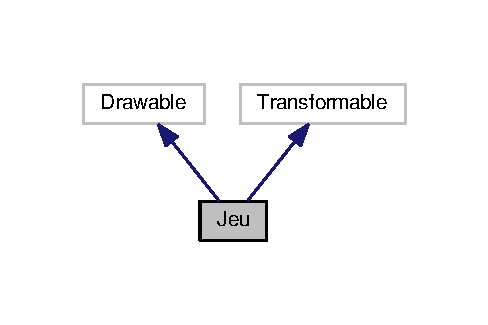
\includegraphics[width=234pt]{class_jeu__inherit__graph}
\end{center}
\end{figure}


Collaboration diagram for Jeu\+:
\nopagebreak
\begin{figure}[H]
\begin{center}
\leavevmode
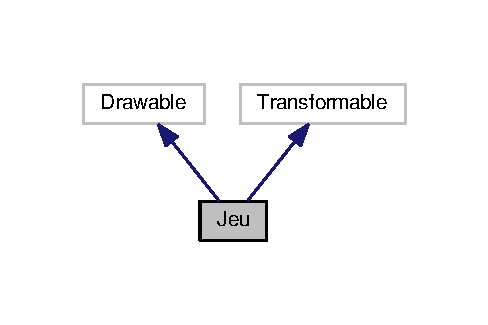
\includegraphics[width=234pt]{class_jeu__coll__graph}
\end{center}
\end{figure}
\subsection*{Public Member Functions}
\begin{DoxyCompactItemize}
\item 
\hyperlink{class_jeu_ab1215a7dd0ff35aab33aa75d35be033d}{Jeu} (\hyperlink{class_tile_map}{Tile\+Map} \&t, \hyperlink{class_personnage}{Personnage} \&p)
\begin{DoxyCompactList}\small\item\em Constructeur. \end{DoxyCompactList}\item 
\hyperlink{class_jeu_a9cd19e73df169d7f09397be61ba8548c}{$\sim$\+Jeu} ()
\begin{DoxyCompactList}\small\item\em Destructeur. \end{DoxyCompactList}\item 
void \hyperlink{class_jeu_ae576e644696381ad0a1c165c6dc789b4}{start} ()
\begin{DoxyCompactList}\small\item\em Lance le jeu. \end{DoxyCompactList}\item 
void \hyperlink{class_jeu_abf2ef17f214900d6a862d9943f2f15c7}{add\+Level} (\hyperlink{class_tile_map}{Tile\+Map} $\ast$t)
\begin{DoxyCompactList}\small\item\em Ajout d'un niveau au \hyperlink{class_jeu}{Jeu}. \end{DoxyCompactList}\item 
\hyperlink{class_tile_map}{Tile\+Map} $\ast$ \hyperlink{class_jeu_ace73ca775ed5e7a13560a541b0c2b8a1}{get\+Current\+Level} () const 
\begin{DoxyCompactList}\small\item\em Récupère le niveau en cours. \end{DoxyCompactList}\item 
const sf\+::\+Font \& \hyperlink{class_jeu_afeedcd4eab224f8bfbd3d34593a06297}{get\+Font} () const 
\begin{DoxyCompactList}\small\item\em Récupère le Font rattachée. \end{DoxyCompactList}\item 
void \hyperlink{class_jeu_ab1e361ec100fae4090ffb062f797b7b5}{set\+State} (\hyperlink{class_state}{State} $\ast$s)
\begin{DoxyCompactList}\small\item\em Setter du \hyperlink{class_state}{State}. \end{DoxyCompactList}\item 
\hyperlink{class_state_level}{State\+Level} $\ast$ \hyperlink{class_jeu_a2632dcd588e4cfb6cc38076cb807190c}{get\+State\+Level} () const 
\begin{DoxyCompactList}\small\item\em Getter du \hyperlink{class_state_level}{State\+Level}. \end{DoxyCompactList}\item 
\hyperlink{class_state_esc_menu}{State\+Esc\+Menu} $\ast$ \hyperlink{class_jeu_af4e8d3d39a32c20fed3e397a6e2cd939}{get\+State\+Esc\+Menu} () const 
\begin{DoxyCompactList}\small\item\em Getter du \hyperlink{class_state_esc_menu}{State\+Esc\+Menu}. \end{DoxyCompactList}\item 
\hyperlink{class_state_main_menu}{State\+Main\+Menu} $\ast$ \hyperlink{class_jeu_a09945f1c10ce230032fcdc3f25d19171}{get\+State\+Main\+Menu} () const 
\begin{DoxyCompactList}\small\item\em Getter du \hyperlink{class_state_main_menu}{State\+Main\+Menu}. \end{DoxyCompactList}\item 
\hyperlink{class_state_stats}{State\+Stats} $\ast$ \hyperlink{class_jeu_a5410b8b324962476890c9a123fc70d90}{get\+State\+Stats} (bool Is\+Level\+Finished) const 
\begin{DoxyCompactList}\small\item\em Getter du get\+State\+Stats. \end{DoxyCompactList}\item 
void \hyperlink{class_jeu_a8bba4f66ac8ea96d51bf889a55e93ffe}{init\+State\+Level} () const 
\begin{DoxyCompactList}\small\item\em Appelle l'initialisation des stats. \end{DoxyCompactList}\item 
bool \hyperlink{class_jeu_a8be6f5df4a2571ded83690a842b8f962}{change\+To\+Next\+Level} ()
\begin{DoxyCompactList}\small\item\em Passe au niveau suivant. \end{DoxyCompactList}\item 
\hyperlink{class_tile_map}{Tile\+Map} $\ast$ \hyperlink{class_jeu_a596d11f5941768eb94a71ffedabdfd03}{reset\+Level} ()
\begin{DoxyCompactList}\small\item\em Reset le level. \end{DoxyCompactList}\item 
void \hyperlink{class_jeu_afd75e6f1113c08b62e9794a9c78425d3}{close} ()
\begin{DoxyCompactList}\small\item\em Enregistre la fermeture de la fenêtre. \end{DoxyCompactList}\item 
void \hyperlink{class_jeu_ac92789bfe84b9a8df297978643b26ed5}{restart\+Char\+Clock} () const 
\begin{DoxyCompactList}\small\item\em Reset le timer du personnage. \end{DoxyCompactList}\end{DoxyCompactItemize}


\subsection{Detailed Description}
Gère tout la fenêtre et les interactions lors d'une partie. 

\subsection{Constructor \& Destructor Documentation}
\hypertarget{class_jeu_ab1215a7dd0ff35aab33aa75d35be033d}{\index{Jeu@{Jeu}!Jeu@{Jeu}}
\index{Jeu@{Jeu}!Jeu@{Jeu}}
\subsubsection[{Jeu}]{\setlength{\rightskip}{0pt plus 5cm}Jeu\+::\+Jeu (
\begin{DoxyParamCaption}
\item[{{\bf Tile\+Map} \&}]{t, }
\item[{{\bf Personnage} \&}]{p}
\end{DoxyParamCaption}
)}}\label{class_jeu_ab1215a7dd0ff35aab33aa75d35be033d}


Constructeur. 

Constructeur de la classe \hyperlink{class_jeu}{Jeu}


\begin{DoxyParams}{Parameters}
{\em t} & \+: \hyperlink{class_tile_map}{Tile\+Map} à générer, p \+: \hyperlink{class_personnage}{Personnage} à jouer. \\
\hline
\end{DoxyParams}
\hypertarget{class_jeu_a9cd19e73df169d7f09397be61ba8548c}{\index{Jeu@{Jeu}!````~Jeu@{$\sim$\+Jeu}}
\index{````~Jeu@{$\sim$\+Jeu}!Jeu@{Jeu}}
\subsubsection[{$\sim$\+Jeu}]{\setlength{\rightskip}{0pt plus 5cm}Jeu\+::$\sim$\+Jeu (
\begin{DoxyParamCaption}
{}
\end{DoxyParamCaption}
)}}\label{class_jeu_a9cd19e73df169d7f09397be61ba8548c}


Destructeur. 

Destructeur de la classe \hyperlink{class_jeu}{Jeu} 

\subsection{Member Function Documentation}
\hypertarget{class_jeu_abf2ef17f214900d6a862d9943f2f15c7}{\index{Jeu@{Jeu}!add\+Level@{add\+Level}}
\index{add\+Level@{add\+Level}!Jeu@{Jeu}}
\subsubsection[{add\+Level}]{\setlength{\rightskip}{0pt plus 5cm}void Jeu\+::add\+Level (
\begin{DoxyParamCaption}
\item[{{\bf Tile\+Map} $\ast$}]{t}
\end{DoxyParamCaption}
)}}\label{class_jeu_abf2ef17f214900d6a862d9943f2f15c7}


Ajout d'un niveau au \hyperlink{class_jeu}{Jeu}. 

Méthode permettant d'ajouter un level depuis une \hyperlink{class_tile_map}{Tile\+Map} au \hyperlink{class_jeu}{Jeu}.


\begin{DoxyParams}{Parameters}
{\em t} & \+: La \hyperlink{class_tile_map}{Tile\+Map} à ajouter comme niveau. \\
\hline
\end{DoxyParams}
\hypertarget{class_jeu_a8be6f5df4a2571ded83690a842b8f962}{\index{Jeu@{Jeu}!change\+To\+Next\+Level@{change\+To\+Next\+Level}}
\index{change\+To\+Next\+Level@{change\+To\+Next\+Level}!Jeu@{Jeu}}
\subsubsection[{change\+To\+Next\+Level}]{\setlength{\rightskip}{0pt plus 5cm}bool Jeu\+::change\+To\+Next\+Level (
\begin{DoxyParamCaption}
{}
\end{DoxyParamCaption}
)}}\label{class_jeu_a8be6f5df4a2571ded83690a842b8f962}


Passe au niveau suivant. 

Si il reste un niveau a charger, alors on le charge en tant que niveau en cours.

\begin{DoxyReturn}{Returns}
Un boolean qui dit si le changement a été effectué. 
\end{DoxyReturn}
\hypertarget{class_jeu_afd75e6f1113c08b62e9794a9c78425d3}{\index{Jeu@{Jeu}!close@{close}}
\index{close@{close}!Jeu@{Jeu}}
\subsubsection[{close}]{\setlength{\rightskip}{0pt plus 5cm}void Jeu\+::close (
\begin{DoxyParamCaption}
{}
\end{DoxyParamCaption}
)}}\label{class_jeu_afd75e6f1113c08b62e9794a9c78425d3}


Enregistre la fermeture de la fenêtre. 

Passe un global bool en false afin d'enregistrer la fermeture de la fenêtr principale. \hypertarget{class_jeu_ace73ca775ed5e7a13560a541b0c2b8a1}{\index{Jeu@{Jeu}!get\+Current\+Level@{get\+Current\+Level}}
\index{get\+Current\+Level@{get\+Current\+Level}!Jeu@{Jeu}}
\subsubsection[{get\+Current\+Level}]{\setlength{\rightskip}{0pt plus 5cm}{\bf Tile\+Map} $\ast$ Jeu\+::get\+Current\+Level (
\begin{DoxyParamCaption}
{}
\end{DoxyParamCaption}
) const}}\label{class_jeu_ace73ca775ed5e7a13560a541b0c2b8a1}


Récupère le niveau en cours. 

Fonction permettant de récupérer la \hyperlink{class_tile_map}{Tile\+Map} du niveau en cours \hypertarget{class_jeu_afeedcd4eab224f8bfbd3d34593a06297}{\index{Jeu@{Jeu}!get\+Font@{get\+Font}}
\index{get\+Font@{get\+Font}!Jeu@{Jeu}}
\subsubsection[{get\+Font}]{\setlength{\rightskip}{0pt plus 5cm}const sf\+::\+Font \& Jeu\+::get\+Font (
\begin{DoxyParamCaption}
{}
\end{DoxyParamCaption}
) const}}\label{class_jeu_afeedcd4eab224f8bfbd3d34593a06297}


Récupère le Font rattachée. 

Récupère la police rattaché au \hyperlink{class_jeu}{Jeu}. \hypertarget{class_jeu_af4e8d3d39a32c20fed3e397a6e2cd939}{\index{Jeu@{Jeu}!get\+State\+Esc\+Menu@{get\+State\+Esc\+Menu}}
\index{get\+State\+Esc\+Menu@{get\+State\+Esc\+Menu}!Jeu@{Jeu}}
\subsubsection[{get\+State\+Esc\+Menu}]{\setlength{\rightskip}{0pt plus 5cm}{\bf State\+Esc\+Menu} $\ast$ Jeu\+::get\+State\+Esc\+Menu (
\begin{DoxyParamCaption}
{}
\end{DoxyParamCaption}
) const}}\label{class_jeu_af4e8d3d39a32c20fed3e397a6e2cd939}


Getter du \hyperlink{class_state_esc_menu}{State\+Esc\+Menu}. 

Renvoi le \hyperlink{class_state_esc_menu}{State\+Esc\+Menu}

\begin{DoxyReturn}{Returns}
Un \hyperlink{class_state_esc_menu}{State\+Esc\+Menu} 
\end{DoxyReturn}
\hypertarget{class_jeu_a2632dcd588e4cfb6cc38076cb807190c}{\index{Jeu@{Jeu}!get\+State\+Level@{get\+State\+Level}}
\index{get\+State\+Level@{get\+State\+Level}!Jeu@{Jeu}}
\subsubsection[{get\+State\+Level}]{\setlength{\rightskip}{0pt plus 5cm}{\bf State\+Level} $\ast$ Jeu\+::get\+State\+Level (
\begin{DoxyParamCaption}
{}
\end{DoxyParamCaption}
) const}}\label{class_jeu_a2632dcd588e4cfb6cc38076cb807190c}


Getter du \hyperlink{class_state_level}{State\+Level}. 

Renvoi le \hyperlink{class_state_level}{State\+Level}

\begin{DoxyReturn}{Returns}
Un \hyperlink{class_state_level}{State\+Level} 
\end{DoxyReturn}
\hypertarget{class_jeu_a09945f1c10ce230032fcdc3f25d19171}{\index{Jeu@{Jeu}!get\+State\+Main\+Menu@{get\+State\+Main\+Menu}}
\index{get\+State\+Main\+Menu@{get\+State\+Main\+Menu}!Jeu@{Jeu}}
\subsubsection[{get\+State\+Main\+Menu}]{\setlength{\rightskip}{0pt plus 5cm}{\bf State\+Main\+Menu}$\ast$ Jeu\+::get\+State\+Main\+Menu (
\begin{DoxyParamCaption}
{}
\end{DoxyParamCaption}
) const}}\label{class_jeu_a09945f1c10ce230032fcdc3f25d19171}


Getter du \hyperlink{class_state_main_menu}{State\+Main\+Menu}. 

/fn State\+Main\+Menu$\ast$ \hyperlink{class_jeu_a09945f1c10ce230032fcdc3f25d19171}{get\+State\+Main\+Menu() const} Renvoi le \hyperlink{class_state_main_menu}{State\+Main\+Menu}

\begin{DoxyReturn}{Returns}
Un \hyperlink{class_state_main_menu}{State\+Main\+Menu} 
\end{DoxyReturn}
\hypertarget{class_jeu_a5410b8b324962476890c9a123fc70d90}{\index{Jeu@{Jeu}!get\+State\+Stats@{get\+State\+Stats}}
\index{get\+State\+Stats@{get\+State\+Stats}!Jeu@{Jeu}}
\subsubsection[{get\+State\+Stats}]{\setlength{\rightskip}{0pt plus 5cm}{\bf State\+Stats}$\ast$ Jeu\+::get\+State\+Stats (
\begin{DoxyParamCaption}
\item[{bool}]{Is\+Level\+Finished}
\end{DoxyParamCaption}
) const}}\label{class_jeu_a5410b8b324962476890c9a123fc70d90}


Getter du get\+State\+Stats. 

/fn get\+State\+Stats$\ast$ \hyperlink{class_jeu_a09945f1c10ce230032fcdc3f25d19171}{get\+State\+Main\+Menu() const} Renvoi le get\+State\+Stats


\begin{DoxyParams}{Parameters}
{\em Is\+Level\+Finished} & \+: bool qui donne l'information si le niveau est finit ou non. \\
\hline
\end{DoxyParams}
\begin{DoxyReturn}{Returns}
Un get\+State\+Stats 
\end{DoxyReturn}
\hypertarget{class_jeu_a8bba4f66ac8ea96d51bf889a55e93ffe}{\index{Jeu@{Jeu}!init\+State\+Level@{init\+State\+Level}}
\index{init\+State\+Level@{init\+State\+Level}!Jeu@{Jeu}}
\subsubsection[{init\+State\+Level}]{\setlength{\rightskip}{0pt plus 5cm}void Jeu\+::init\+State\+Level (
\begin{DoxyParamCaption}
{}
\end{DoxyParamCaption}
) const}}\label{class_jeu_a8bba4f66ac8ea96d51bf889a55e93ffe}


Appelle l'initialisation des stats. 

Appelle la procédure init du \hyperlink{class_state_level}{State\+Level}. \hypertarget{class_jeu_a596d11f5941768eb94a71ffedabdfd03}{\index{Jeu@{Jeu}!reset\+Level@{reset\+Level}}
\index{reset\+Level@{reset\+Level}!Jeu@{Jeu}}
\subsubsection[{reset\+Level}]{\setlength{\rightskip}{0pt plus 5cm}{\bf Tile\+Map} $\ast$ Jeu\+::reset\+Level (
\begin{DoxyParamCaption}
{}
\end{DoxyParamCaption}
)}}\label{class_jeu_a596d11f5941768eb94a71ffedabdfd03}


Reset le level. 

La \hyperlink{class_tile_map}{Tile\+Map} reset. \hypertarget{class_jeu_ac92789bfe84b9a8df297978643b26ed5}{\index{Jeu@{Jeu}!restart\+Char\+Clock@{restart\+Char\+Clock}}
\index{restart\+Char\+Clock@{restart\+Char\+Clock}!Jeu@{Jeu}}
\subsubsection[{restart\+Char\+Clock}]{\setlength{\rightskip}{0pt plus 5cm}Jeu\+::restart\+Char\+Clock (
\begin{DoxyParamCaption}
{}
\end{DoxyParamCaption}
) const}}\label{class_jeu_ac92789bfe84b9a8df297978643b26ed5}


Reset le timer du personnage. 

Appelle la fonction restart\+Clock du personnage. \hypertarget{class_jeu_ab1e361ec100fae4090ffb062f797b7b5}{\index{Jeu@{Jeu}!set\+State@{set\+State}}
\index{set\+State@{set\+State}!Jeu@{Jeu}}
\subsubsection[{set\+State}]{\setlength{\rightskip}{0pt plus 5cm}void Jeu\+::set\+State (
\begin{DoxyParamCaption}
\item[{{\bf State} $\ast$}]{s}
\end{DoxyParamCaption}
)}}\label{class_jeu_ab1e361ec100fae4090ffb062f797b7b5}


Setter du \hyperlink{class_state}{State}. 

Permet de modifier l'état du \hyperlink{class_state}{State}.


\begin{DoxyParams}{Parameters}
{\em s} & \+: \hyperlink{class_state}{State} à modifier. \\
\hline
\end{DoxyParams}
\hypertarget{class_jeu_ae576e644696381ad0a1c165c6dc789b4}{\index{Jeu@{Jeu}!start@{start}}
\index{start@{start}!Jeu@{Jeu}}
\subsubsection[{start}]{\setlength{\rightskip}{0pt plus 5cm}void Jeu\+::start (
\begin{DoxyParamCaption}
{}
\end{DoxyParamCaption}
)}}\label{class_jeu_ae576e644696381ad0a1c165c6dc789b4}


Lance le jeu. 

Ouvre la fenêtre et lance le jeu 

The documentation for this class was generated from the following file\+:\begin{DoxyCompactItemize}
\item 
\hyperlink{_jeu_8hpp}{Jeu.\+hpp}\end{DoxyCompactItemize}

\hypertarget{class_jumper}{\section{Jumper Class Reference}
\label{class_jumper}\index{Jumper@{Jumper}}
}


Classe gérant les ennemi qui marchent.  




{\ttfamily \#include $<$Jumper.\+hpp$>$}



Inheritance diagram for Jumper\+:
\nopagebreak
\begin{figure}[H]
\begin{center}
\leavevmode
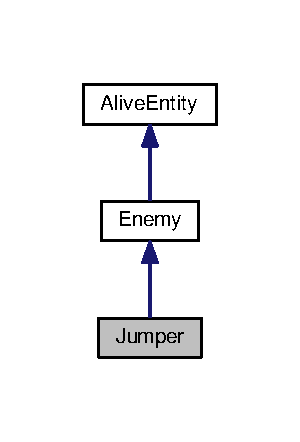
\includegraphics[width=144pt]{class_jumper__inherit__graph}
\end{center}
\end{figure}


Collaboration diagram for Jumper\+:
\nopagebreak
\begin{figure}[H]
\begin{center}
\leavevmode
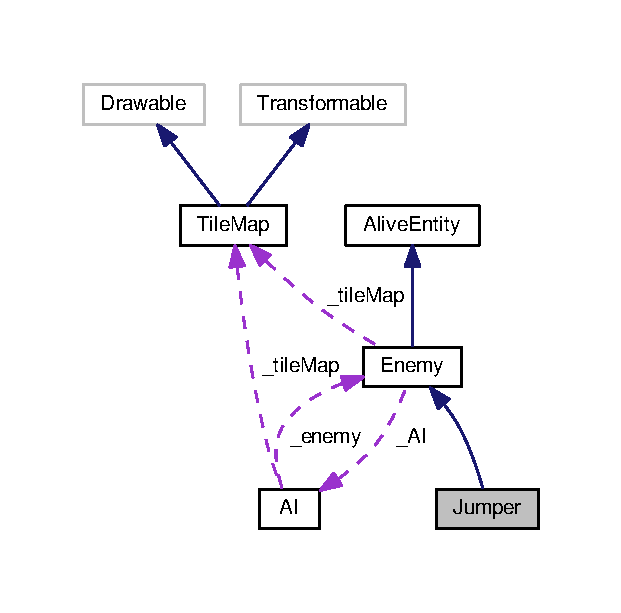
\includegraphics[width=298pt]{class_jumper__coll__graph}
\end{center}
\end{figure}
\subsection*{Public Member Functions}
\begin{DoxyCompactItemize}
\item 
\hyperlink{class_jumper_aa3c6e89077ba3a080af168097279cc6f}{Jumper} (const sf\+::\+Vector2f \&taille, \hyperlink{class_tile_map}{Tile\+Map} \&tilemap, int speed, int jump\+Height)
\begin{DoxyCompactList}\small\item\em Constructeur du \hyperlink{class_jumper}{Jumper}. \end{DoxyCompactList}\item 
\hypertarget{class_jumper_ad77cd99be7134fd48c30bd265b4a377e}{{\bfseries Jumper} (const sf\+::\+Vector2f \&taille, const sf\+::\+Vector2f \&position, \hyperlink{class_tile_map}{Tile\+Map} \&tilemap, int speed, int jump\+Height)}\label{class_jumper_ad77cd99be7134fd48c30bd265b4a377e}

\item 
\hypertarget{class_jumper_ab4a5eb758e0668d6cee17e96e0ec1344}{{\bfseries Jumper} (const sf\+::\+Vector2f \&taille, \hyperlink{class_tile_map}{Tile\+Map} \&tilemap, const \hyperlink{class_personnage}{Personnage} \&perso, int speed, int jump\+Height)}\label{class_jumper_ab4a5eb758e0668d6cee17e96e0ec1344}

\item 
\hyperlink{class_enemy}{Enemy} $\ast$ \hyperlink{class_jumper_aa28b8e0acc2f4fa045b29359692fe4ac}{clone} ()
\begin{DoxyCompactList}\small\item\em Clone le \hyperlink{class_jumper}{Jumper}. \end{DoxyCompactList}\item 
int \hyperlink{class_jumper_a36d7e9b3b3718e50c983be709ed359e3}{get\+Speed} () const 
\begin{DoxyCompactList}\small\item\em Getter de la vitesse du l'ennemi. \end{DoxyCompactList}\item 
int \hyperlink{class_jumper_a87f2e80d2d819ab4d2d339401ae18a54}{get\+Jump\+Height} () const 
\begin{DoxyCompactList}\small\item\em Getter de la hauteur de saut de l'ennemi. \end{DoxyCompactList}\item 
\hypertarget{class_jumper_a3b827b7900f19e8c078401dc148e0f7b}{unsigned int {\bfseries get\+Reward} () const }\label{class_jumper_a3b827b7900f19e8c078401dc148e0f7b}

\end{DoxyCompactItemize}
\subsection*{Additional Inherited Members}


\subsection{Detailed Description}
Classe gérant les ennemi qui marchent. 

\subsection{Constructor \& Destructor Documentation}
\hypertarget{class_jumper_aa3c6e89077ba3a080af168097279cc6f}{\index{Jumper@{Jumper}!Jumper@{Jumper}}
\index{Jumper@{Jumper}!Jumper@{Jumper}}
\subsubsection[{Jumper}]{\setlength{\rightskip}{0pt plus 5cm}Jumper\+::\+Jumper (
\begin{DoxyParamCaption}
\item[{const sf\+::\+Vector2f \&}]{taille, }
\item[{{\bf Tile\+Map} \&}]{tilemap, }
\item[{int}]{speed, }
\item[{int}]{jump\+Height}
\end{DoxyParamCaption}
)}}\label{class_jumper_aa3c6e89077ba3a080af168097279cc6f}


Constructeur du \hyperlink{class_jumper}{Jumper}. 

Constructeur du \hyperlink{class_jumper}{Jumper}


\begin{DoxyParams}{Parameters}
{\em taille} & Taille de la hitbox \\
\hline
{\em tilemap} & Map sur laquelle est l'ennemi \\
\hline
{\em int} & Sa vitesse, en pixels par frame \\
\hline
{\em int} & Sa hauteur de saut, poussée en Y \\
\hline
\end{DoxyParams}


\subsection{Member Function Documentation}
\hypertarget{class_jumper_aa28b8e0acc2f4fa045b29359692fe4ac}{\index{Jumper@{Jumper}!clone@{clone}}
\index{clone@{clone}!Jumper@{Jumper}}
\subsubsection[{clone}]{\setlength{\rightskip}{0pt plus 5cm}{\bf Enemy} $\ast$ Jumper\+::clone (
\begin{DoxyParamCaption}
{}
\end{DoxyParamCaption}
)\hspace{0.3cm}{\ttfamily [virtual]}}}\label{class_jumper_aa28b8e0acc2f4fa045b29359692fe4ac}


Clone le \hyperlink{class_jumper}{Jumper}. 

Créer un nouveau \hyperlink{class_jumper}{Jumper} avec les même caractéristiques.

\begin{DoxyReturn}{Returns}
Un clone du \hyperlink{class_jumper}{Jumper} existant 
\end{DoxyReturn}


Implements \hyperlink{class_enemy_a21d5d2f97aa7406a985fd0ca3f3b1028}{Enemy}.

\hypertarget{class_jumper_a87f2e80d2d819ab4d2d339401ae18a54}{\index{Jumper@{Jumper}!get\+Jump\+Height@{get\+Jump\+Height}}
\index{get\+Jump\+Height@{get\+Jump\+Height}!Jumper@{Jumper}}
\subsubsection[{get\+Jump\+Height}]{\setlength{\rightskip}{0pt plus 5cm}int Jumper\+::get\+Jump\+Height (
\begin{DoxyParamCaption}
{}
\end{DoxyParamCaption}
) const}}\label{class_jumper_a87f2e80d2d819ab4d2d339401ae18a54}


Getter de la hauteur de saut de l'ennemi. 

Getter de la Hauteur de saut de l'ennemi, soit la pourssée en Y lors du saut \begin{DoxyReturn}{Returns}
La valeur de la poussée en Y 
\end{DoxyReturn}
\hypertarget{class_jumper_a36d7e9b3b3718e50c983be709ed359e3}{\index{Jumper@{Jumper}!get\+Speed@{get\+Speed}}
\index{get\+Speed@{get\+Speed}!Jumper@{Jumper}}
\subsubsection[{get\+Speed}]{\setlength{\rightskip}{0pt plus 5cm}int Jumper\+::get\+Speed (
\begin{DoxyParamCaption}
{}
\end{DoxyParamCaption}
) const}}\label{class_jumper_a36d7e9b3b3718e50c983be709ed359e3}


Getter de la vitesse du l'ennemi. 

Getter de la vitesse de l'ennemi, en pixels par frame \begin{DoxyReturn}{Returns}
Le deplacement de l'ennemi à chaque frame 
\end{DoxyReturn}


The documentation for this class was generated from the following file\+:\begin{DoxyCompactItemize}
\item 
\hyperlink{_jumper_8hpp}{Jumper.\+hpp}\end{DoxyCompactItemize}

\hypertarget{class_personnage}{\section{Personnage Class Reference}
\label{class_personnage}\index{Personnage@{Personnage}}
}


Classe définissant un personnage.  




{\ttfamily \#include $<$Personnage.\+hpp$>$}



Inheritance diagram for Personnage\+:
\nopagebreak
\begin{figure}[H]
\begin{center}
\leavevmode
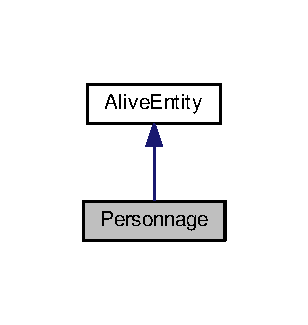
\includegraphics[width=148pt]{class_personnage__inherit__graph}
\end{center}
\end{figure}


Collaboration diagram for Personnage\+:
\nopagebreak
\begin{figure}[H]
\begin{center}
\leavevmode
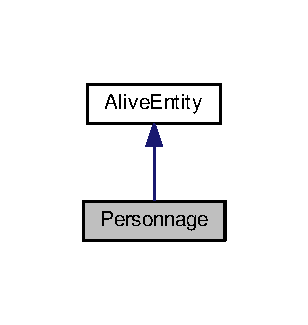
\includegraphics[width=148pt]{class_personnage__coll__graph}
\end{center}
\end{figure}
\subsection*{Public Member Functions}
\begin{DoxyCompactItemize}
\item 
\hyperlink{class_personnage_ae031dfa471739621e0a908e4946ea6ad}{Personnage} (const sf\+::\+Vector2f \&taille, sf\+::\+Image \&i, sf\+::\+Texture \&t)
\begin{DoxyCompactList}\small\item\em Constructeur. \end{DoxyCompactList}\item 
\hyperlink{class_personnage_a05bdf2a469885bb1fbb6c2e8f98972ab}{$\sim$\+Personnage} ()
\begin{DoxyCompactList}\small\item\em Destructeur. \end{DoxyCompactList}\item 
void \hyperlink{class_personnage_acddd15a955d84943f587ba9f799c14b0}{add\+Mouvement} (const sf\+::\+Vector2f \&mvt)
\begin{DoxyCompactList}\small\item\em Modifie le mouvement en cours, en vérifiant qu'il reste dans des limites définies. \end{DoxyCompactList}\item 
void \hyperlink{class_personnage_a23827b5a59cc4a5372c01ec45d3c5fb7}{move} (sf\+::\+Vector2f v)
\begin{DoxyCompactList}\small\item\em Bouge le \hyperlink{class_personnage}{Personnage}. \end{DoxyCompactList}\item 
void \hyperlink{class_personnage_abfd05381e426b6b68eaa51309e66736c}{restart\+Clock} ()
\begin{DoxyCompactList}\small\item\em relance la clock du personnage \end{DoxyCompactList}\item 
sf\+::\+Time \hyperlink{class_personnage_aa226c2909c41a07f5fdf884f293e7d9b}{get\+Elapsed\+Time} () const 
\begin{DoxyCompactList}\small\item\em Récupère le temps écoulé \end{DoxyCompactList}\item 
void \hyperlink{class_personnage_a1fb547b3bdbd33437a7a07f8479dced3}{flip\+Right} ()
\begin{DoxyCompactList}\small\item\em Tourne la texture vers la droite. \end{DoxyCompactList}\item 
void \hyperlink{class_personnage_a01ec8b39bc3052b8b47e86f2f29d14a5}{flip\+Left} ()
\begin{DoxyCompactList}\small\item\em Tourne la texture à gauche. \end{DoxyCompactList}\item 
unsigned int \hyperlink{class_personnage_ae1f499ed5540c639c974c8727b8b56d7}{get\+Current\+Kill} () const 
\begin{DoxyCompactList}\small\item\em Getter de Current\+Kill. \end{DoxyCompactList}\item 
unsigned int \hyperlink{class_personnage_ad9dcc6e0c92a08b0947a2ec4adf1add3}{get\+Current\+Score} () const 
\begin{DoxyCompactList}\small\item\em Getter de Current\+Score. \end{DoxyCompactList}\item 
unsigned int \hyperlink{class_personnage_a85ee701a050e63d79e10df70ebfb9ec1}{get\+Total\+Kill} () const 
\begin{DoxyCompactList}\small\item\em Getter de Total\+Kill. \end{DoxyCompactList}\item 
unsigned int \hyperlink{class_personnage_a1f4117a6232487b0b59fff62038a3bf2}{get\+Total\+Score} () const 
\begin{DoxyCompactList}\small\item\em Getter de Total\+Score. \end{DoxyCompactList}\item 
void \hyperlink{class_personnage_a2ace7870446cd275ecb2d83d7cc1c65c}{set\+Current\+Kill} (unsigned int k)
\begin{DoxyCompactList}\small\item\em Setter de Current\+Kill. \end{DoxyCompactList}\item 
void \hyperlink{class_personnage_a2530fa41c83f03a1d65bdc70b5baf25a}{set\+Current\+Score} (unsigned int s)
\begin{DoxyCompactList}\small\item\em Setter de Current\+Score. \end{DoxyCompactList}\item 
void \hyperlink{class_personnage_a8f1a4f017745593d8fc5d371d38c8ae4}{set\+Total\+Kill} (unsigned int k)
\begin{DoxyCompactList}\small\item\em Setter de Total\+Kill. \end{DoxyCompactList}\item 
void \hyperlink{class_personnage_a90d388a1ee096f74a3fd000f5607d1fc}{set\+Total\+Score} (unsigned int s)
\begin{DoxyCompactList}\small\item\em Setter de Total\+Score. \end{DoxyCompactList}\end{DoxyCompactItemize}
\subsection*{Additional Inherited Members}


\subsection{Detailed Description}
Classe définissant un personnage. 

\subsection{Constructor \& Destructor Documentation}
\hypertarget{class_personnage_ae031dfa471739621e0a908e4946ea6ad}{\index{Personnage@{Personnage}!Personnage@{Personnage}}
\index{Personnage@{Personnage}!Personnage@{Personnage}}
\subsubsection[{Personnage}]{\setlength{\rightskip}{0pt plus 5cm}Personnage\+::\+Personnage (
\begin{DoxyParamCaption}
\item[{const sf\+::\+Vector2f \&}]{taille, }
\item[{sf\+::\+Image \&}]{i, }
\item[{sf\+::\+Texture \&}]{t}
\end{DoxyParamCaption}
)}}\label{class_personnage_ae031dfa471739621e0a908e4946ea6ad}


Constructeur. 

Constructeur de la classe \hyperlink{class_personnage}{Personnage}.


\begin{DoxyParams}{Parameters}
{\em taille} & \+: taille (en 2\+D) du personnage, i \+: image du personnage, t \+: texture du personnage. \\
\hline
\end{DoxyParams}
\hypertarget{class_personnage_a05bdf2a469885bb1fbb6c2e8f98972ab}{\index{Personnage@{Personnage}!````~Personnage@{$\sim$\+Personnage}}
\index{````~Personnage@{$\sim$\+Personnage}!Personnage@{Personnage}}
\subsubsection[{$\sim$\+Personnage}]{\setlength{\rightskip}{0pt plus 5cm}Personnage\+::$\sim$\+Personnage (
\begin{DoxyParamCaption}
{}
\end{DoxyParamCaption}
)}}\label{class_personnage_a05bdf2a469885bb1fbb6c2e8f98972ab}


Destructeur. 

Destructeur de la classe \hyperlink{class_personnage}{Personnage}. 

\subsection{Member Function Documentation}
\hypertarget{class_personnage_acddd15a955d84943f587ba9f799c14b0}{\index{Personnage@{Personnage}!add\+Mouvement@{add\+Mouvement}}
\index{add\+Mouvement@{add\+Mouvement}!Personnage@{Personnage}}
\subsubsection[{add\+Mouvement}]{\setlength{\rightskip}{0pt plus 5cm}void Personnage\+::add\+Mouvement (
\begin{DoxyParamCaption}
\item[{const sf\+::\+Vector2f \&}]{mvt}
\end{DoxyParamCaption}
)}}\label{class_personnage_acddd15a955d84943f587ba9f799c14b0}


Modifie le mouvement en cours, en vérifiant qu'il reste dans des limites définies. 

Modifie le mouvement du personnage en fonction des anciens paramètres et des limites fixées par le jeu.


\begin{DoxyParams}{Parameters}
{\em v} & \+: vecteur 2 dimensions qui affectera le mouvement en cours \\
\hline
\end{DoxyParams}
\hypertarget{class_personnage_a01ec8b39bc3052b8b47e86f2f29d14a5}{\index{Personnage@{Personnage}!flip\+Left@{flip\+Left}}
\index{flip\+Left@{flip\+Left}!Personnage@{Personnage}}
\subsubsection[{flip\+Left}]{\setlength{\rightskip}{0pt plus 5cm}void Personnage\+::flip\+Left (
\begin{DoxyParamCaption}
{}
\end{DoxyParamCaption}
)}}\label{class_personnage_a01ec8b39bc3052b8b47e86f2f29d14a5}


Tourne la texture à gauche. 

Fait regarder le canard à gauche \hypertarget{class_personnage_a1fb547b3bdbd33437a7a07f8479dced3}{\index{Personnage@{Personnage}!flip\+Right@{flip\+Right}}
\index{flip\+Right@{flip\+Right}!Personnage@{Personnage}}
\subsubsection[{flip\+Right}]{\setlength{\rightskip}{0pt plus 5cm}void Personnage\+::flip\+Right (
\begin{DoxyParamCaption}
{}
\end{DoxyParamCaption}
)}}\label{class_personnage_a1fb547b3bdbd33437a7a07f8479dced3}


Tourne la texture vers la droite. 

Fait regarder le canard à droite \hypertarget{class_personnage_ae1f499ed5540c639c974c8727b8b56d7}{\index{Personnage@{Personnage}!get\+Current\+Kill@{get\+Current\+Kill}}
\index{get\+Current\+Kill@{get\+Current\+Kill}!Personnage@{Personnage}}
\subsubsection[{get\+Current\+Kill}]{\setlength{\rightskip}{0pt plus 5cm}unsigned int Personnage\+::get\+Current\+Kill (
\begin{DoxyParamCaption}
{}
\end{DoxyParamCaption}
) const}}\label{class_personnage_ae1f499ed5540c639c974c8727b8b56d7}


Getter de Current\+Kill. 

Récupère le nombre de kill fait par le personnage sur le niveau en cours

\begin{DoxyReturn}{Returns}
Le nombre de kill 
\end{DoxyReturn}
\hypertarget{class_personnage_ad9dcc6e0c92a08b0947a2ec4adf1add3}{\index{Personnage@{Personnage}!get\+Current\+Score@{get\+Current\+Score}}
\index{get\+Current\+Score@{get\+Current\+Score}!Personnage@{Personnage}}
\subsubsection[{get\+Current\+Score}]{\setlength{\rightskip}{0pt plus 5cm}unsigned int Personnage\+::get\+Current\+Score (
\begin{DoxyParamCaption}
{}
\end{DoxyParamCaption}
) const}}\label{class_personnage_ad9dcc6e0c92a08b0947a2ec4adf1add3}


Getter de Current\+Score. 

Récupère le score fait par le personnage sur le niveau en cours

\begin{DoxyReturn}{Returns}
Le score 
\end{DoxyReturn}
\hypertarget{class_personnage_aa226c2909c41a07f5fdf884f293e7d9b}{\index{Personnage@{Personnage}!get\+Elapsed\+Time@{get\+Elapsed\+Time}}
\index{get\+Elapsed\+Time@{get\+Elapsed\+Time}!Personnage@{Personnage}}
\subsubsection[{get\+Elapsed\+Time}]{\setlength{\rightskip}{0pt plus 5cm}sf\+::\+Time Personnage\+::get\+Elapsed\+Time (
\begin{DoxyParamCaption}
{}
\end{DoxyParamCaption}
) const}}\label{class_personnage_aa226c2909c41a07f5fdf884f293e7d9b}


Récupère le temps écoulé 

Retourne le temps passé depuis la dernière ré-\/initialisation de la clock

\begin{DoxyReturn}{Returns}
La durée qui s'est écoulé depuis le début du niveau 
\end{DoxyReturn}
\hypertarget{class_personnage_a85ee701a050e63d79e10df70ebfb9ec1}{\index{Personnage@{Personnage}!get\+Total\+Kill@{get\+Total\+Kill}}
\index{get\+Total\+Kill@{get\+Total\+Kill}!Personnage@{Personnage}}
\subsubsection[{get\+Total\+Kill}]{\setlength{\rightskip}{0pt plus 5cm}unsigned int Personnage\+::get\+Total\+Kill (
\begin{DoxyParamCaption}
{}
\end{DoxyParamCaption}
) const}}\label{class_personnage_a85ee701a050e63d79e10df70ebfb9ec1}


Getter de Total\+Kill. 

Récupère le nombre de kill fait par le personnage sur la totalité des niveaux

\begin{DoxyReturn}{Returns}
Le nombre de kill total 
\end{DoxyReturn}
\hypertarget{class_personnage_a1f4117a6232487b0b59fff62038a3bf2}{\index{Personnage@{Personnage}!get\+Total\+Score@{get\+Total\+Score}}
\index{get\+Total\+Score@{get\+Total\+Score}!Personnage@{Personnage}}
\subsubsection[{get\+Total\+Score}]{\setlength{\rightskip}{0pt plus 5cm}unsigned int Personnage\+::get\+Total\+Score (
\begin{DoxyParamCaption}
{}
\end{DoxyParamCaption}
) const}}\label{class_personnage_a1f4117a6232487b0b59fff62038a3bf2}


Getter de Total\+Score. 

Récupère le score fait par le personnage sur la totalité des niveaux

\begin{DoxyReturn}{Returns}
Le score total 
\end{DoxyReturn}
\hypertarget{class_personnage_a23827b5a59cc4a5372c01ec45d3c5fb7}{\index{Personnage@{Personnage}!move@{move}}
\index{move@{move}!Personnage@{Personnage}}
\subsubsection[{move}]{\setlength{\rightskip}{0pt plus 5cm}void Personnage\+::move (
\begin{DoxyParamCaption}
\item[{sf\+::\+Vector2f}]{v}
\end{DoxyParamCaption}
)}}\label{class_personnage_a23827b5a59cc4a5372c01ec45d3c5fb7}


Bouge le \hyperlink{class_personnage}{Personnage}. 

Déplace le \hyperlink{class_personnage}{Personnage} en lui appliquant les frottements


\begin{DoxyParams}{Parameters}
{\em v} & \+: Vector2f définissant le mouvement. \\
\hline
\end{DoxyParams}
\hypertarget{class_personnage_abfd05381e426b6b68eaa51309e66736c}{\index{Personnage@{Personnage}!restart\+Clock@{restart\+Clock}}
\index{restart\+Clock@{restart\+Clock}!Personnage@{Personnage}}
\subsubsection[{restart\+Clock}]{\setlength{\rightskip}{0pt plus 5cm}void Personnage\+::restart\+Clock (
\begin{DoxyParamCaption}
{}
\end{DoxyParamCaption}
)}}\label{class_personnage_abfd05381e426b6b68eaa51309e66736c}


relance la clock du personnage 

Appelle un fonction de S\+F\+M\+L qui reset la clock. \hypertarget{class_personnage_a2ace7870446cd275ecb2d83d7cc1c65c}{\index{Personnage@{Personnage}!set\+Current\+Kill@{set\+Current\+Kill}}
\index{set\+Current\+Kill@{set\+Current\+Kill}!Personnage@{Personnage}}
\subsubsection[{set\+Current\+Kill}]{\setlength{\rightskip}{0pt plus 5cm}void Personnage\+::set\+Current\+Kill (
\begin{DoxyParamCaption}
\item[{unsigned int}]{k}
\end{DoxyParamCaption}
)}}\label{class_personnage_a2ace7870446cd275ecb2d83d7cc1c65c}


Setter de Current\+Kill. 

Initialise le nombre de kill


\begin{DoxyParams}{Parameters}
{\em k} & \+: valeur d'initialisation \\
\hline
\end{DoxyParams}
\hypertarget{class_personnage_a2530fa41c83f03a1d65bdc70b5baf25a}{\index{Personnage@{Personnage}!set\+Current\+Score@{set\+Current\+Score}}
\index{set\+Current\+Score@{set\+Current\+Score}!Personnage@{Personnage}}
\subsubsection[{set\+Current\+Score}]{\setlength{\rightskip}{0pt plus 5cm}void Personnage\+::set\+Current\+Score (
\begin{DoxyParamCaption}
\item[{unsigned int}]{s}
\end{DoxyParamCaption}
)}}\label{class_personnage_a2530fa41c83f03a1d65bdc70b5baf25a}


Setter de Current\+Score. 

Initialise le score


\begin{DoxyParams}{Parameters}
{\em s} & \+: valeur d'initialisation \\
\hline
\end{DoxyParams}
\hypertarget{class_personnage_a8f1a4f017745593d8fc5d371d38c8ae4}{\index{Personnage@{Personnage}!set\+Total\+Kill@{set\+Total\+Kill}}
\index{set\+Total\+Kill@{set\+Total\+Kill}!Personnage@{Personnage}}
\subsubsection[{set\+Total\+Kill}]{\setlength{\rightskip}{0pt plus 5cm}void Personnage\+::set\+Total\+Kill (
\begin{DoxyParamCaption}
\item[{unsigned int}]{k}
\end{DoxyParamCaption}
)}}\label{class_personnage_a8f1a4f017745593d8fc5d371d38c8ae4}


Setter de Total\+Kill. 

Initialise le nombre de total de kill


\begin{DoxyParams}{Parameters}
{\em k} & \+: valeur d'initialisation \\
\hline
\end{DoxyParams}
\hypertarget{class_personnage_a90d388a1ee096f74a3fd000f5607d1fc}{\index{Personnage@{Personnage}!set\+Total\+Score@{set\+Total\+Score}}
\index{set\+Total\+Score@{set\+Total\+Score}!Personnage@{Personnage}}
\subsubsection[{set\+Total\+Score}]{\setlength{\rightskip}{0pt plus 5cm}void Personnage\+::set\+Total\+Score (
\begin{DoxyParamCaption}
\item[{unsigned int}]{s}
\end{DoxyParamCaption}
)}}\label{class_personnage_a90d388a1ee096f74a3fd000f5607d1fc}


Setter de Total\+Score. 

Initialise le score total


\begin{DoxyParams}{Parameters}
{\em s} & \+: valeur d'initialisation \\
\hline
\end{DoxyParams}


The documentation for this class was generated from the following file\+:\begin{DoxyCompactItemize}
\item 
\hyperlink{_personnage_8hpp}{Personnage.\+hpp}\end{DoxyCompactItemize}

\hypertarget{class_spawner}{\section{Spawner Class Reference}
\label{class_spawner}\index{Spawner@{Spawner}}
}
\subsection*{Public Member Functions}
\begin{DoxyCompactItemize}
\item 
\hyperlink{class_spawner_a4b2a9b9f860c7756b3781dca43542dac}{Spawner} (\hyperlink{class_enemy}{Enemy} $\ast$prototype)
\begin{DoxyCompactList}\small\item\em Constructeur. \end{DoxyCompactList}\item 
\hyperlink{class_enemy}{Enemy} $\ast$ \hyperlink{class_spawner_a7a426313f071f61fa823e42254fc20e6}{spawn\+Enemy} ()
\begin{DoxyCompactList}\small\item\em Clone l'\hyperlink{class_enemy}{Enemy} contenu dans le spawner. \end{DoxyCompactList}\end{DoxyCompactItemize}


\subsection{Constructor \& Destructor Documentation}
\hypertarget{class_spawner_a4b2a9b9f860c7756b3781dca43542dac}{\index{Spawner@{Spawner}!Spawner@{Spawner}}
\index{Spawner@{Spawner}!Spawner@{Spawner}}
\subsubsection[{Spawner}]{\setlength{\rightskip}{0pt plus 5cm}Spawner\+::\+Spawner (
\begin{DoxyParamCaption}
\item[{{\bf Enemy} $\ast$}]{prototype}
\end{DoxyParamCaption}
)}}\label{class_spawner_a4b2a9b9f860c7756b3781dca43542dac}


Constructeur. 

Constructeur de la classe \hyperlink{class_spawner}{Spawner}


\begin{DoxyParams}{Parameters}
{\em prototype} & \+: \hyperlink{class_enemy}{Enemy} à cloner \\
\hline
\end{DoxyParams}


\subsection{Member Function Documentation}
\hypertarget{class_spawner_a7a426313f071f61fa823e42254fc20e6}{\index{Spawner@{Spawner}!spawn\+Enemy@{spawn\+Enemy}}
\index{spawn\+Enemy@{spawn\+Enemy}!Spawner@{Spawner}}
\subsubsection[{spawn\+Enemy}]{\setlength{\rightskip}{0pt plus 5cm}{\bf Enemy} $\ast$ Spawner\+::spawn\+Enemy (
\begin{DoxyParamCaption}
{}
\end{DoxyParamCaption}
)}}\label{class_spawner_a7a426313f071f61fa823e42254fc20e6}


Clone l'\hyperlink{class_enemy}{Enemy} contenu dans le spawner. 

Appelle la fonction clone du prototype

\begin{DoxyReturn}{Returns}
Un nouvel \hyperlink{class_enemy}{Enemy} 
\end{DoxyReturn}


The documentation for this class was generated from the following file\+:\begin{DoxyCompactItemize}
\item 
\hyperlink{_spawner_8hpp}{Spawner.\+hpp}\end{DoxyCompactItemize}

\hypertarget{class_state}{\section{State Class Reference}
\label{class_state}\index{State@{State}}
}


Interface du \hyperlink{class_state}{State}.  




{\ttfamily \#include $<$State.\+hpp$>$}



Inheritance diagram for State\+:
\nopagebreak
\begin{figure}[H]
\begin{center}
\leavevmode
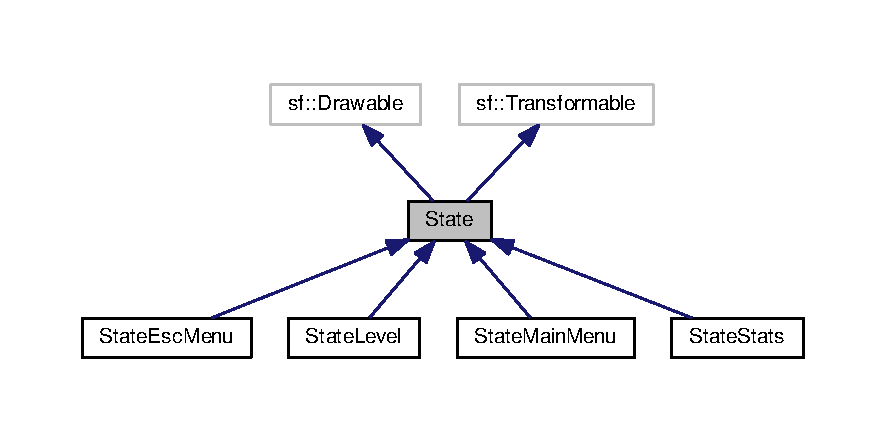
\includegraphics[width=350pt]{class_state__inherit__graph}
\end{center}
\end{figure}


Collaboration diagram for State\+:
\nopagebreak
\begin{figure}[H]
\begin{center}
\leavevmode
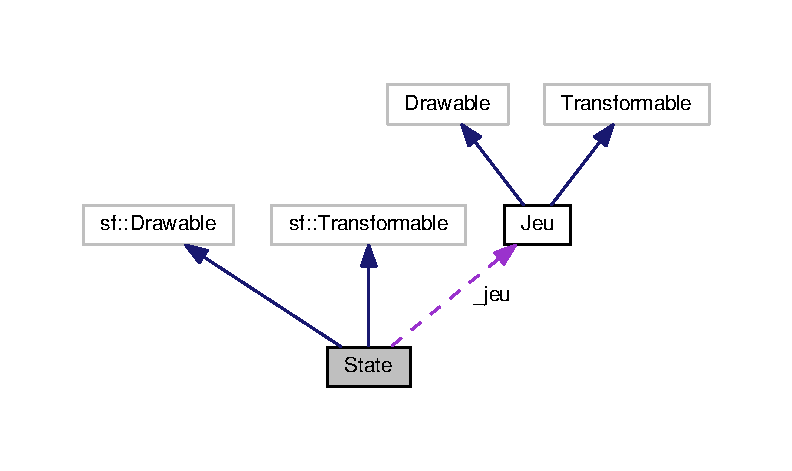
\includegraphics[width=350pt]{class_state__coll__graph}
\end{center}
\end{figure}
\subsection*{Public Member Functions}
\begin{DoxyCompactItemize}
\item 
\hyperlink{class_state_a83d07567e1a24f802e5cb85ab55f3569}{State} (\hyperlink{class_jeu}{Jeu} $\ast$jeu)
\begin{DoxyCompactList}\small\item\em Constructeur. \end{DoxyCompactList}\item 
\hyperlink{class_state_afab438d92b90dc18d194dbd9c9c8bab3}{$\sim$\+State} ()
\begin{DoxyCompactList}\small\item\em Destructeur. \end{DoxyCompactList}\item 
virtual void \hyperlink{class_state_a7e115388c37a05ee165a395f3119d685}{draw} (sf\+::\+Render\+Target \&target, sf\+::\+Render\+States states) const =0
\begin{DoxyCompactList}\small\item\em Dessine un objet. \end{DoxyCompactList}\item 
virtual void \hyperlink{class_state_abe618d6673b514d93ccd6e4ced6ed992}{init} ()
\begin{DoxyCompactList}\small\item\em initialise les coord. du spawn du personnage \end{DoxyCompactList}\item 
virtual void \hyperlink{class_state_a8e992fd4ce2009a2f736ec674dadec3e}{press\+Space} ()
\begin{DoxyCompactList}\small\item\em Action à effectuer quand Espace est appuyé \end{DoxyCompactList}\item 
virtual void \hyperlink{class_state_ab3837b57093899dbdb323540c75a79e8}{press\+Up} ()=0
\begin{DoxyCompactList}\small\item\em Action à effectuer quand la touche Haut est appuyé \end{DoxyCompactList}\item 
virtual void \hyperlink{class_state_a0f77b5ab3a8cbdd35fef9d0d5b414e1f}{press\+Down} ()=0
\begin{DoxyCompactList}\small\item\em Action à effectuer quand la touche Bas est appuyé \end{DoxyCompactList}\item 
virtual void \hyperlink{class_state_a2717680ed591de1f09250b6c7548209a}{press\+Esc} ()
\begin{DoxyCompactList}\small\item\em Action à effectuer quand la touche Echap est appuyé \end{DoxyCompactList}\item 
virtual void \hyperlink{class_state_aa2633a4a944f0b68bfb3bbf7b8029dcc}{press\+Left} ()
\begin{DoxyCompactList}\small\item\em Action à effectuer quand la touche Gauche est appuyé \end{DoxyCompactList}\item 
virtual void \hyperlink{class_state_a8af37cc742f499101673fd42425a113f}{press\+Right} ()
\begin{DoxyCompactList}\small\item\em Action à effectuer quand la touche Droite est appuyé \end{DoxyCompactList}\item 
virtual void \hyperlink{class_state_a62d60bde66bc403c40ece17e069a616d}{press\+Enter} ()
\begin{DoxyCompactList}\small\item\em Action à effectuer quand la touche Entrée est appuyé \end{DoxyCompactList}\item 
virtual void \hyperlink{class_state_a1c39ad3bdaa33864ee474b6be0e3e44d}{update} ()
\begin{DoxyCompactList}\small\item\em Update le niveau en cours. \end{DoxyCompactList}\end{DoxyCompactItemize}
\subsection*{Protected Attributes}
\begin{DoxyCompactItemize}
\item 
\hypertarget{class_state_aa155bffcebfe54c1f3787f596379a6bf}{\hyperlink{class_jeu}{Jeu} $\ast$ {\bfseries \+\_\+jeu}}\label{class_state_aa155bffcebfe54c1f3787f596379a6bf}

\end{DoxyCompactItemize}


\subsection{Detailed Description}
Interface du \hyperlink{class_state}{State}. 

\hyperlink{class_state}{State} 

\subsection{Constructor \& Destructor Documentation}
\hypertarget{class_state_a83d07567e1a24f802e5cb85ab55f3569}{\index{State@{State}!State@{State}}
\index{State@{State}!State@{State}}
\subsubsection[{State}]{\setlength{\rightskip}{0pt plus 5cm}State\+::\+State (
\begin{DoxyParamCaption}
\item[{{\bf Jeu} $\ast$}]{jeu}
\end{DoxyParamCaption}
)}}\label{class_state_a83d07567e1a24f802e5cb85ab55f3569}


Constructeur. 

Constructeur de la classe \hyperlink{class_state}{State}


\begin{DoxyParams}{Parameters}
{\em jeu} & \+: \hyperlink{class_jeu}{Jeu} sur lequel le Pattern \hyperlink{class_state}{State} s'applique \\
\hline
\end{DoxyParams}
\hypertarget{class_state_afab438d92b90dc18d194dbd9c9c8bab3}{\index{State@{State}!````~State@{$\sim$\+State}}
\index{````~State@{$\sim$\+State}!State@{State}}
\subsubsection[{$\sim$\+State}]{\setlength{\rightskip}{0pt plus 5cm}State\+::$\sim$\+State (
\begin{DoxyParamCaption}
{}
\end{DoxyParamCaption}
)}}\label{class_state_afab438d92b90dc18d194dbd9c9c8bab3}


Destructeur. 

Destructeur de la classe \hyperlink{class_state}{State} 

\subsection{Member Function Documentation}
\hypertarget{class_state_a7e115388c37a05ee165a395f3119d685}{\index{State@{State}!draw@{draw}}
\index{draw@{draw}!State@{State}}
\subsubsection[{draw}]{\setlength{\rightskip}{0pt plus 5cm}void State\+::draw (
\begin{DoxyParamCaption}
\item[{sf\+::\+Render\+Target \&}]{target, }
\item[{sf\+::\+Render\+States}]{states}
\end{DoxyParamCaption}
) const\hspace{0.3cm}{\ttfamily [pure virtual]}}}\label{class_state_a7e115388c37a05ee165a395f3119d685}


Dessine un objet. 

Prends un objet target et le dessine.


\begin{DoxyParams}{Parameters}
{\em target} & \+: objet à dessiner, states \+: applique la transformation (S\+F\+M\+L Function) \\
\hline
\end{DoxyParams}


Implemented in \hyperlink{class_state_main_menu_ae372daf9ed9b53da4c23c01d4a7787a4}{State\+Main\+Menu}, \hyperlink{class_state_stats_ae8ee0b50f030d3057b0635158c170715}{State\+Stats}, \hyperlink{class_state_esc_menu_a6ab405b062d3caad840036c4d38d895b}{State\+Esc\+Menu}, and \hyperlink{class_state_level_a8e7ec8788b8c1992781fe135a5dc5f7d}{State\+Level}.

\hypertarget{class_state_abe618d6673b514d93ccd6e4ced6ed992}{\index{State@{State}!init@{init}}
\index{init@{init}!State@{State}}
\subsubsection[{init}]{\setlength{\rightskip}{0pt plus 5cm}void State\+::init (
\begin{DoxyParamCaption}
{}
\end{DoxyParamCaption}
)\hspace{0.3cm}{\ttfamily [virtual]}}}\label{class_state_abe618d6673b514d93ccd6e4ced6ed992}


initialise les coord. du spawn du personnage 

Initialise pour les niveaux les coordonnées du \hyperlink{class_personnage}{Personnage} jouable. 

Reimplemented in \hyperlink{class_state_level_a901fd0b511f35b0af1b6e88ceedc6748}{State\+Level}.

\hypertarget{class_state_a0f77b5ab3a8cbdd35fef9d0d5b414e1f}{\index{State@{State}!press\+Down@{press\+Down}}
\index{press\+Down@{press\+Down}!State@{State}}
\subsubsection[{press\+Down}]{\setlength{\rightskip}{0pt plus 5cm}void State\+::press\+Down (
\begin{DoxyParamCaption}
{}
\end{DoxyParamCaption}
)\hspace{0.3cm}{\ttfamily [pure virtual]}}}\label{class_state_a0f77b5ab3a8cbdd35fef9d0d5b414e1f}


Action à effectuer quand la touche Bas est appuyé 

Gère les actions rattachées à la touche Bas. 

Implemented in \hyperlink{class_state_level_abc115526af37fd93a87b0eba998de49e}{State\+Level}, \hyperlink{class_state_main_menu_a90c547b9d2aae731a752c71fb7c0ab4a}{State\+Main\+Menu}, \hyperlink{class_state_stats_ac19acb64e561b57a02a826328aa827f6}{State\+Stats}, and \hyperlink{class_state_esc_menu_a412f7eead9e8103468abc5c099e50a69}{State\+Esc\+Menu}.

\hypertarget{class_state_a62d60bde66bc403c40ece17e069a616d}{\index{State@{State}!press\+Enter@{press\+Enter}}
\index{press\+Enter@{press\+Enter}!State@{State}}
\subsubsection[{press\+Enter}]{\setlength{\rightskip}{0pt plus 5cm}void State\+::press\+Enter (
\begin{DoxyParamCaption}
{}
\end{DoxyParamCaption}
)\hspace{0.3cm}{\ttfamily [virtual]}}}\label{class_state_a62d60bde66bc403c40ece17e069a616d}


Action à effectuer quand la touche Entrée est appuyé 

Gère les actions rattachées à la touche Entrée. 

Reimplemented in \hyperlink{class_state_main_menu_a25dac2e7223f8f36a9e4f372bb25b702}{State\+Main\+Menu}, \hyperlink{class_state_stats_a12a42d0bc1a2d43c48d76fe9e1e0fdfd}{State\+Stats}, and \hyperlink{class_state_esc_menu_ab791b49eaf53562f13eb4d11378821c2}{State\+Esc\+Menu}.

\hypertarget{class_state_a2717680ed591de1f09250b6c7548209a}{\index{State@{State}!press\+Esc@{press\+Esc}}
\index{press\+Esc@{press\+Esc}!State@{State}}
\subsubsection[{press\+Esc}]{\setlength{\rightskip}{0pt plus 5cm}void State\+::press\+Esc (
\begin{DoxyParamCaption}
{}
\end{DoxyParamCaption}
)\hspace{0.3cm}{\ttfamily [virtual]}}}\label{class_state_a2717680ed591de1f09250b6c7548209a}


Action à effectuer quand la touche Echap est appuyé 

Gère les actions rattachées à la touche Echap. 

Reimplemented in \hyperlink{class_state_level_ab733bd4321a90d8171710dc895ee982a}{State\+Level}, and \hyperlink{class_state_esc_menu_ae9075e15b4ff41ecc16ed1b38b73ef2c}{State\+Esc\+Menu}.

\hypertarget{class_state_aa2633a4a944f0b68bfb3bbf7b8029dcc}{\index{State@{State}!press\+Left@{press\+Left}}
\index{press\+Left@{press\+Left}!State@{State}}
\subsubsection[{press\+Left}]{\setlength{\rightskip}{0pt plus 5cm}void State\+::press\+Left (
\begin{DoxyParamCaption}
{}
\end{DoxyParamCaption}
)\hspace{0.3cm}{\ttfamily [virtual]}}}\label{class_state_aa2633a4a944f0b68bfb3bbf7b8029dcc}


Action à effectuer quand la touche Gauche est appuyé 

Gère les actions rattachées à la touche Gauche. 

Reimplemented in \hyperlink{class_state_level_a0b4b1cdf50b6fa528468eea65ba09156}{State\+Level}.

\hypertarget{class_state_a8af37cc742f499101673fd42425a113f}{\index{State@{State}!press\+Right@{press\+Right}}
\index{press\+Right@{press\+Right}!State@{State}}
\subsubsection[{press\+Right}]{\setlength{\rightskip}{0pt plus 5cm}void State\+::press\+Right (
\begin{DoxyParamCaption}
{}
\end{DoxyParamCaption}
)\hspace{0.3cm}{\ttfamily [virtual]}}}\label{class_state_a8af37cc742f499101673fd42425a113f}


Action à effectuer quand la touche Droite est appuyé 

Gère les actions rattachées à la touche Droite. 

Reimplemented in \hyperlink{class_state_level_a6ec0177bd71f7f9e60dd4896322959b1}{State\+Level}.

\hypertarget{class_state_a8e992fd4ce2009a2f736ec674dadec3e}{\index{State@{State}!press\+Space@{press\+Space}}
\index{press\+Space@{press\+Space}!State@{State}}
\subsubsection[{press\+Space}]{\setlength{\rightskip}{0pt plus 5cm}void State\+::press\+Space (
\begin{DoxyParamCaption}
{}
\end{DoxyParamCaption}
)\hspace{0.3cm}{\ttfamily [virtual]}}}\label{class_state_a8e992fd4ce2009a2f736ec674dadec3e}


Action à effectuer quand Espace est appuyé 

Gère les actions rattachées à la barre d'espace. 

Reimplemented in \hyperlink{class_state_level_ab83986dcc97a8a923009b7c6a2aec6f6}{State\+Level}.

\hypertarget{class_state_ab3837b57093899dbdb323540c75a79e8}{\index{State@{State}!press\+Up@{press\+Up}}
\index{press\+Up@{press\+Up}!State@{State}}
\subsubsection[{press\+Up}]{\setlength{\rightskip}{0pt plus 5cm}void State\+::press\+Up (
\begin{DoxyParamCaption}
{}
\end{DoxyParamCaption}
)\hspace{0.3cm}{\ttfamily [pure virtual]}}}\label{class_state_ab3837b57093899dbdb323540c75a79e8}


Action à effectuer quand la touche Haut est appuyé 

Gère les actions rattachées à la touche Haut. 

Implemented in \hyperlink{class_state_level_aa16ac397de41618dc276a4984ace536c}{State\+Level}, \hyperlink{class_state_main_menu_a714cb2def73b1146ad862e667b6996ee}{State\+Main\+Menu}, \hyperlink{class_state_stats_a4fd39389aa2debf191b718dc750ccf8a}{State\+Stats}, and \hyperlink{class_state_esc_menu_a455940a22b887bf3289d5837d089d6b5}{State\+Esc\+Menu}.

\hypertarget{class_state_a1c39ad3bdaa33864ee474b6be0e3e44d}{\index{State@{State}!update@{update}}
\index{update@{update}!State@{State}}
\subsubsection[{update}]{\setlength{\rightskip}{0pt plus 5cm}void State\+::update (
\begin{DoxyParamCaption}
{}
\end{DoxyParamCaption}
)\hspace{0.3cm}{\ttfamily [virtual]}}}\label{class_state_a1c39ad3bdaa33864ee474b6be0e3e44d}


Update le niveau en cours. 

Vérifie les collisions, mets à jour la caméra On vérifie aussi la fin de niveau, les conditions de mort Et enfin on bouge les ennemis. 

Reimplemented in \hyperlink{class_state_level_ab2adefb4d13c7534096f9744eb183577}{State\+Level}.



The documentation for this class was generated from the following file\+:\begin{DoxyCompactItemize}
\item 
\hyperlink{_state_8hpp}{State.\+hpp}\end{DoxyCompactItemize}

\hypertarget{class_state_esc_menu}{\section{State\+Esc\+Menu Class Reference}
\label{class_state_esc_menu}\index{State\+Esc\+Menu@{State\+Esc\+Menu}}
}


Etat Esc\+Menu rattaché au Pattern \hyperlink{class_state}{State}.  




{\ttfamily \#include $<$State\+Esc\+Menu.\+hpp$>$}



Inheritance diagram for State\+Esc\+Menu\+:
\nopagebreak
\begin{figure}[H]
\begin{center}
\leavevmode
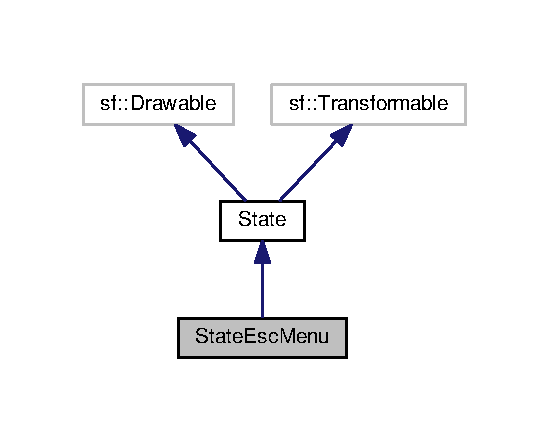
\includegraphics[width=263pt]{class_state_esc_menu__inherit__graph}
\end{center}
\end{figure}


Collaboration diagram for State\+Esc\+Menu\+:
\nopagebreak
\begin{figure}[H]
\begin{center}
\leavevmode
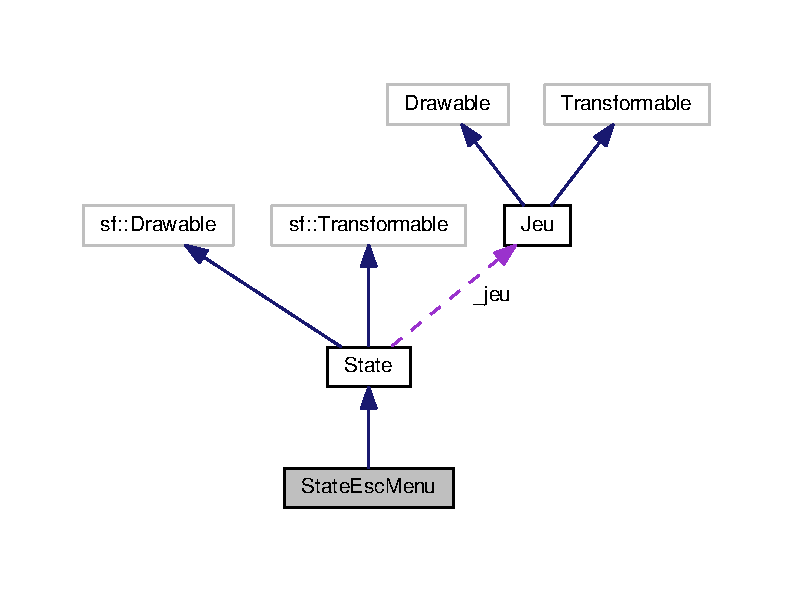
\includegraphics[width=350pt]{class_state_esc_menu__coll__graph}
\end{center}
\end{figure}
\subsection*{Public Member Functions}
\begin{DoxyCompactItemize}
\item 
\hyperlink{class_state_esc_menu_ac73762653b28be7e912641712d774a15}{State\+Esc\+Menu} (\hyperlink{class_jeu}{Jeu} $\ast$jeu)
\begin{DoxyCompactList}\small\item\em Constructeur. \end{DoxyCompactList}\item 
\hyperlink{class_state_esc_menu_a5eb2aad9f7cc85e772859fe95d7f28a7}{$\sim$\+State\+Esc\+Menu} ()
\begin{DoxyCompactList}\small\item\em Destructeur. \end{DoxyCompactList}\item 
virtual void \hyperlink{class_state_esc_menu_a6ab405b062d3caad840036c4d38d895b}{draw} (sf\+::\+Render\+Target \&target, sf\+::\+Render\+States states) const 
\begin{DoxyCompactList}\small\item\em Dessine un objet. \end{DoxyCompactList}\item 
virtual void \hyperlink{class_state_esc_menu_a455940a22b887bf3289d5837d089d6b5}{press\+Up} ()
\begin{DoxyCompactList}\small\item\em Action à effectuer quand la touche Haut est appuyé \end{DoxyCompactList}\item 
virtual void \hyperlink{class_state_esc_menu_a412f7eead9e8103468abc5c099e50a69}{press\+Down} ()
\begin{DoxyCompactList}\small\item\em Action à effectuer quand la touche Bas est appuyé \end{DoxyCompactList}\item 
virtual void \hyperlink{class_state_esc_menu_ab791b49eaf53562f13eb4d11378821c2}{press\+Enter} ()
\begin{DoxyCompactList}\small\item\em Action à effectuer quand Entrée est appuyé \end{DoxyCompactList}\item 
virtual void \hyperlink{class_state_esc_menu_ae9075e15b4ff41ecc16ed1b38b73ef2c}{press\+Esc} ()
\begin{DoxyCompactList}\small\item\em Action à effectuer quand la touche Echap est appuyé \end{DoxyCompactList}\end{DoxyCompactItemize}
\subsection*{Additional Inherited Members}


\subsection{Detailed Description}
Etat Esc\+Menu rattaché au Pattern \hyperlink{class_state}{State}. 

\hyperlink{class_state_esc_menu}{State\+Esc\+Menu} 

\subsection{Constructor \& Destructor Documentation}
\hypertarget{class_state_esc_menu_ac73762653b28be7e912641712d774a15}{\index{State\+Esc\+Menu@{State\+Esc\+Menu}!State\+Esc\+Menu@{State\+Esc\+Menu}}
\index{State\+Esc\+Menu@{State\+Esc\+Menu}!State\+Esc\+Menu@{State\+Esc\+Menu}}
\subsubsection[{State\+Esc\+Menu}]{\setlength{\rightskip}{0pt plus 5cm}State\+Esc\+Menu\+::\+State\+Esc\+Menu (
\begin{DoxyParamCaption}
\item[{{\bf Jeu} $\ast$}]{jeu}
\end{DoxyParamCaption}
)}}\label{class_state_esc_menu_ac73762653b28be7e912641712d774a15}


Constructeur. 

Constructeur de la classe \hyperlink{class_state}{State}


\begin{DoxyParams}{Parameters}
{\em jeu} & \+: \hyperlink{class_jeu}{Jeu} sur lequel le Pattern \hyperlink{class_state}{State} s'applique \\
\hline
\end{DoxyParams}
\hypertarget{class_state_esc_menu_a5eb2aad9f7cc85e772859fe95d7f28a7}{\index{State\+Esc\+Menu@{State\+Esc\+Menu}!````~State\+Esc\+Menu@{$\sim$\+State\+Esc\+Menu}}
\index{````~State\+Esc\+Menu@{$\sim$\+State\+Esc\+Menu}!State\+Esc\+Menu@{State\+Esc\+Menu}}
\subsubsection[{$\sim$\+State\+Esc\+Menu}]{\setlength{\rightskip}{0pt plus 5cm}State\+Esc\+Menu\+::$\sim$\+State\+Esc\+Menu (
\begin{DoxyParamCaption}
{}
\end{DoxyParamCaption}
)}}\label{class_state_esc_menu_a5eb2aad9f7cc85e772859fe95d7f28a7}


Destructeur. 

Destructeur de la classe \hyperlink{class_state}{State} 

\subsection{Member Function Documentation}
\hypertarget{class_state_esc_menu_a6ab405b062d3caad840036c4d38d895b}{\index{State\+Esc\+Menu@{State\+Esc\+Menu}!draw@{draw}}
\index{draw@{draw}!State\+Esc\+Menu@{State\+Esc\+Menu}}
\subsubsection[{draw}]{\setlength{\rightskip}{0pt plus 5cm}void State\+Esc\+Menu\+::draw (
\begin{DoxyParamCaption}
\item[{sf\+::\+Render\+Target \&}]{target, }
\item[{sf\+::\+Render\+States}]{states}
\end{DoxyParamCaption}
) const\hspace{0.3cm}{\ttfamily [virtual]}}}\label{class_state_esc_menu_a6ab405b062d3caad840036c4d38d895b}


Dessine un objet. 

Prends un objet target et le dessine.


\begin{DoxyParams}{Parameters}
{\em target} & \+: objet à dessiner, states \+: applique la transformation (S\+F\+M\+L Function) \\
\hline
\end{DoxyParams}


Implements \hyperlink{class_state_a7e115388c37a05ee165a395f3119d685}{State}.

\hypertarget{class_state_esc_menu_a412f7eead9e8103468abc5c099e50a69}{\index{State\+Esc\+Menu@{State\+Esc\+Menu}!press\+Down@{press\+Down}}
\index{press\+Down@{press\+Down}!State\+Esc\+Menu@{State\+Esc\+Menu}}
\subsubsection[{press\+Down}]{\setlength{\rightskip}{0pt plus 5cm}void State\+Esc\+Menu\+::press\+Down (
\begin{DoxyParamCaption}
{}
\end{DoxyParamCaption}
)\hspace{0.3cm}{\ttfamily [virtual]}}}\label{class_state_esc_menu_a412f7eead9e8103468abc5c099e50a69}


Action à effectuer quand la touche Bas est appuyé 

Gère les actions rattachées à la touche Bas. 

Implements \hyperlink{class_state_a0f77b5ab3a8cbdd35fef9d0d5b414e1f}{State}.

\hypertarget{class_state_esc_menu_ab791b49eaf53562f13eb4d11378821c2}{\index{State\+Esc\+Menu@{State\+Esc\+Menu}!press\+Enter@{press\+Enter}}
\index{press\+Enter@{press\+Enter}!State\+Esc\+Menu@{State\+Esc\+Menu}}
\subsubsection[{press\+Enter}]{\setlength{\rightskip}{0pt plus 5cm}void State\+Esc\+Menu\+::press\+Enter (
\begin{DoxyParamCaption}
{}
\end{DoxyParamCaption}
)\hspace{0.3cm}{\ttfamily [virtual]}}}\label{class_state_esc_menu_ab791b49eaf53562f13eb4d11378821c2}


Action à effectuer quand Entrée est appuyé 

Gère les actions rattachées à la touhce Entrée. 

Reimplemented from \hyperlink{class_state_a62d60bde66bc403c40ece17e069a616d}{State}.

\hypertarget{class_state_esc_menu_ae9075e15b4ff41ecc16ed1b38b73ef2c}{\index{State\+Esc\+Menu@{State\+Esc\+Menu}!press\+Esc@{press\+Esc}}
\index{press\+Esc@{press\+Esc}!State\+Esc\+Menu@{State\+Esc\+Menu}}
\subsubsection[{press\+Esc}]{\setlength{\rightskip}{0pt plus 5cm}void State\+Esc\+Menu\+::press\+Esc (
\begin{DoxyParamCaption}
{}
\end{DoxyParamCaption}
)\hspace{0.3cm}{\ttfamily [virtual]}}}\label{class_state_esc_menu_ae9075e15b4ff41ecc16ed1b38b73ef2c}


Action à effectuer quand la touche Echap est appuyé 

Gère les actions rattachées à la touche Echap. 

Reimplemented from \hyperlink{class_state_a2717680ed591de1f09250b6c7548209a}{State}.

\hypertarget{class_state_esc_menu_a455940a22b887bf3289d5837d089d6b5}{\index{State\+Esc\+Menu@{State\+Esc\+Menu}!press\+Up@{press\+Up}}
\index{press\+Up@{press\+Up}!State\+Esc\+Menu@{State\+Esc\+Menu}}
\subsubsection[{press\+Up}]{\setlength{\rightskip}{0pt plus 5cm}void State\+Esc\+Menu\+::press\+Up (
\begin{DoxyParamCaption}
{}
\end{DoxyParamCaption}
)\hspace{0.3cm}{\ttfamily [virtual]}}}\label{class_state_esc_menu_a455940a22b887bf3289d5837d089d6b5}


Action à effectuer quand la touche Haut est appuyé 

Gère les actions rattachées à la touche Haut. 

Implements \hyperlink{class_state_ab3837b57093899dbdb323540c75a79e8}{State}.



The documentation for this class was generated from the following file\+:\begin{DoxyCompactItemize}
\item 
\hyperlink{_state_esc_menu_8hpp}{State\+Esc\+Menu.\+hpp}\end{DoxyCompactItemize}

\hypertarget{class_state_level}{\section{State\+Level Class Reference}
\label{class_state_level}\index{State\+Level@{State\+Level}}
}


Etat \hyperlink{class_state_level}{State\+Level} rattaché au Pattern \hyperlink{class_state}{State}.  




{\ttfamily \#include $<$State\+Level.\+hpp$>$}



Inheritance diagram for State\+Level\+:
\nopagebreak
\begin{figure}[H]
\begin{center}
\leavevmode
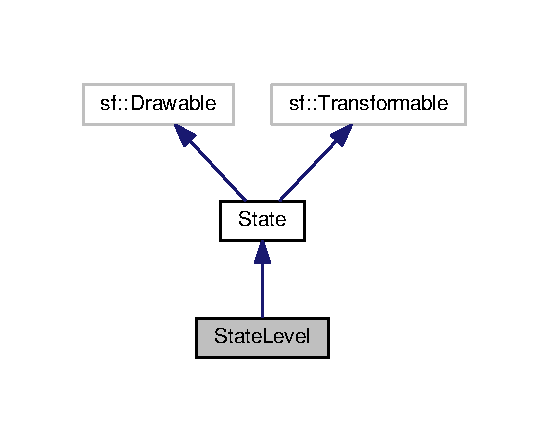
\includegraphics[width=263pt]{class_state_level__inherit__graph}
\end{center}
\end{figure}


Collaboration diagram for State\+Level\+:
\nopagebreak
\begin{figure}[H]
\begin{center}
\leavevmode
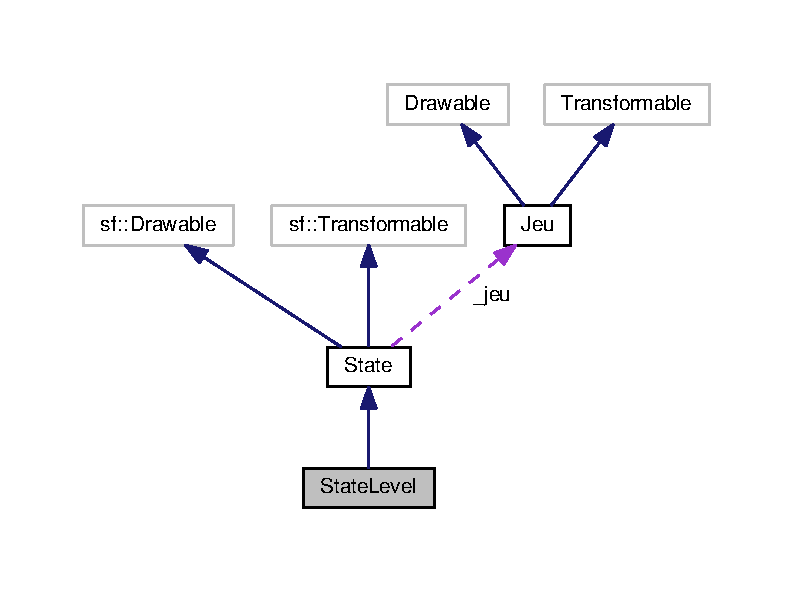
\includegraphics[width=350pt]{class_state_level__coll__graph}
\end{center}
\end{figure}
\subsection*{Public Member Functions}
\begin{DoxyCompactItemize}
\item 
\hyperlink{class_state_level_a08ef66f8eb0ed452eaeb6cf80cae0b4a}{State\+Level} (\hyperlink{class_jeu}{Jeu} $\ast$jeu, \hyperlink{class_tile_map}{Tile\+Map} $\ast$tilemap, \hyperlink{class_personnage}{Personnage} \&perso)
\begin{DoxyCompactList}\small\item\em Constructeur. \end{DoxyCompactList}\item 
virtual void \hyperlink{class_state_level_a8e7ec8788b8c1992781fe135a5dc5f7d}{draw} (sf\+::\+Render\+Target \&target, sf\+::\+Render\+States states) const 
\begin{DoxyCompactList}\small\item\em Dessine un objet. \end{DoxyCompactList}\item 
virtual void \hyperlink{class_state_level_a901fd0b511f35b0af1b6e88ceedc6748}{init} ()
\begin{DoxyCompactList}\small\item\em initialise les coord. du spawn du personnage \end{DoxyCompactList}\item 
virtual void \hyperlink{class_state_level_aefa35ceeb1aa1b391392f38a71af4402}{set\+Level} (\hyperlink{class_tile_map}{Tile\+Map} $\ast$t)
\begin{DoxyCompactList}\small\item\em Setter de la \hyperlink{class_tile_map}{Tile\+Map}. \end{DoxyCompactList}\item 
virtual void \hyperlink{class_state_level_ab83986dcc97a8a923009b7c6a2aec6f6}{press\+Space} ()
\begin{DoxyCompactList}\small\item\em Action à effectuer quand Espace est appuyé \end{DoxyCompactList}\item 
virtual void \hyperlink{class_state_level_aa16ac397de41618dc276a4984ace536c}{press\+Up} ()
\begin{DoxyCompactList}\small\item\em Action à effectuer quand la touche Haut est appuyé \end{DoxyCompactList}\item 
virtual void \hyperlink{class_state_level_abc115526af37fd93a87b0eba998de49e}{press\+Down} ()
\begin{DoxyCompactList}\small\item\em Action à effectuer quand la touche Bas est appuyé \end{DoxyCompactList}\item 
virtual void \hyperlink{class_state_level_ab733bd4321a90d8171710dc895ee982a}{press\+Esc} ()
\begin{DoxyCompactList}\small\item\em Action à effectuer quand la touche Echap est appuyé \end{DoxyCompactList}\item 
virtual void \hyperlink{class_state_level_a0b4b1cdf50b6fa528468eea65ba09156}{press\+Left} ()
\begin{DoxyCompactList}\small\item\em Action à effectuer quand la touche Gauche est appuyé \end{DoxyCompactList}\item 
virtual void \hyperlink{class_state_level_a6ec0177bd71f7f9e60dd4896322959b1}{press\+Right} ()
\begin{DoxyCompactList}\small\item\em Action à effectuer quand la touche Droite est appuyé \end{DoxyCompactList}\item 
void \hyperlink{class_state_level_ab2adefb4d13c7534096f9744eb183577}{update} ()
\begin{DoxyCompactList}\small\item\em Update le niveau en cours. \end{DoxyCompactList}\end{DoxyCompactItemize}
\subsection*{Additional Inherited Members}


\subsection{Detailed Description}
Etat \hyperlink{class_state_level}{State\+Level} rattaché au Pattern \hyperlink{class_state}{State}. 

\hyperlink{class_state_level}{State\+Level} 

\subsection{Constructor \& Destructor Documentation}
\hypertarget{class_state_level_a08ef66f8eb0ed452eaeb6cf80cae0b4a}{\index{State\+Level@{State\+Level}!State\+Level@{State\+Level}}
\index{State\+Level@{State\+Level}!State\+Level@{State\+Level}}
\subsubsection[{State\+Level}]{\setlength{\rightskip}{0pt plus 5cm}State\+Level\+::\+State\+Level (
\begin{DoxyParamCaption}
\item[{{\bf Jeu} $\ast$}]{jeu, }
\item[{{\bf Tile\+Map} $\ast$}]{tilemap, }
\item[{{\bf Personnage} \&}]{perso}
\end{DoxyParamCaption}
)}}\label{class_state_level_a08ef66f8eb0ed452eaeb6cf80cae0b4a}


Constructeur. 

Constructeur de la classe \hyperlink{class_state}{State}


\begin{DoxyParams}{Parameters}
{\em jeu} & \+: \hyperlink{class_jeu}{Jeu} sur lequel le Pattern \hyperlink{class_state}{State} s'applique, perso \+: \hyperlink{class_personnage}{Personnage} jouable \\
\hline
\end{DoxyParams}


\subsection{Member Function Documentation}
\hypertarget{class_state_level_a8e7ec8788b8c1992781fe135a5dc5f7d}{\index{State\+Level@{State\+Level}!draw@{draw}}
\index{draw@{draw}!State\+Level@{State\+Level}}
\subsubsection[{draw}]{\setlength{\rightskip}{0pt plus 5cm}void State\+Level\+::draw (
\begin{DoxyParamCaption}
\item[{sf\+::\+Render\+Target \&}]{target, }
\item[{sf\+::\+Render\+States}]{states}
\end{DoxyParamCaption}
) const\hspace{0.3cm}{\ttfamily [virtual]}}}\label{class_state_level_a8e7ec8788b8c1992781fe135a5dc5f7d}


Dessine un objet. 

Prends un objet target et le dessine.


\begin{DoxyParams}{Parameters}
{\em target} & \+: objet à dessiner, states \+: applique la transformation (S\+F\+M\+L Function) \\
\hline
\end{DoxyParams}


Implements \hyperlink{class_state_a7e115388c37a05ee165a395f3119d685}{State}.

\hypertarget{class_state_level_a901fd0b511f35b0af1b6e88ceedc6748}{\index{State\+Level@{State\+Level}!init@{init}}
\index{init@{init}!State\+Level@{State\+Level}}
\subsubsection[{init}]{\setlength{\rightskip}{0pt plus 5cm}void State\+Level\+::init (
\begin{DoxyParamCaption}
{}
\end{DoxyParamCaption}
)\hspace{0.3cm}{\ttfamily [virtual]}}}\label{class_state_level_a901fd0b511f35b0af1b6e88ceedc6748}


initialise les coord. du spawn du personnage 

Initialise pour les niveaux les coordonnées du \hyperlink{class_personnage}{Personnage} jouable. 

Reimplemented from \hyperlink{class_state_abe618d6673b514d93ccd6e4ced6ed992}{State}.

\hypertarget{class_state_level_abc115526af37fd93a87b0eba998de49e}{\index{State\+Level@{State\+Level}!press\+Down@{press\+Down}}
\index{press\+Down@{press\+Down}!State\+Level@{State\+Level}}
\subsubsection[{press\+Down}]{\setlength{\rightskip}{0pt plus 5cm}void State\+Level\+::press\+Down (
\begin{DoxyParamCaption}
{}
\end{DoxyParamCaption}
)\hspace{0.3cm}{\ttfamily [virtual]}}}\label{class_state_level_abc115526af37fd93a87b0eba998de49e}


Action à effectuer quand la touche Bas est appuyé 

Gère les actions rattachées à la touche Bas. 

Implements \hyperlink{class_state_a0f77b5ab3a8cbdd35fef9d0d5b414e1f}{State}.

\hypertarget{class_state_level_ab733bd4321a90d8171710dc895ee982a}{\index{State\+Level@{State\+Level}!press\+Esc@{press\+Esc}}
\index{press\+Esc@{press\+Esc}!State\+Level@{State\+Level}}
\subsubsection[{press\+Esc}]{\setlength{\rightskip}{0pt plus 5cm}void State\+Level\+::press\+Esc (
\begin{DoxyParamCaption}
{}
\end{DoxyParamCaption}
)\hspace{0.3cm}{\ttfamily [virtual]}}}\label{class_state_level_ab733bd4321a90d8171710dc895ee982a}


Action à effectuer quand la touche Echap est appuyé 

Gère les actions rattachées à la touche Echap. 

Reimplemented from \hyperlink{class_state_a2717680ed591de1f09250b6c7548209a}{State}.

\hypertarget{class_state_level_a0b4b1cdf50b6fa528468eea65ba09156}{\index{State\+Level@{State\+Level}!press\+Left@{press\+Left}}
\index{press\+Left@{press\+Left}!State\+Level@{State\+Level}}
\subsubsection[{press\+Left}]{\setlength{\rightskip}{0pt plus 5cm}void State\+Level\+::press\+Left (
\begin{DoxyParamCaption}
{}
\end{DoxyParamCaption}
)\hspace{0.3cm}{\ttfamily [virtual]}}}\label{class_state_level_a0b4b1cdf50b6fa528468eea65ba09156}


Action à effectuer quand la touche Gauche est appuyé 

Gère les actions rattachées à la touche Gauche. 

Reimplemented from \hyperlink{class_state_aa2633a4a944f0b68bfb3bbf7b8029dcc}{State}.

\hypertarget{class_state_level_a6ec0177bd71f7f9e60dd4896322959b1}{\index{State\+Level@{State\+Level}!press\+Right@{press\+Right}}
\index{press\+Right@{press\+Right}!State\+Level@{State\+Level}}
\subsubsection[{press\+Right}]{\setlength{\rightskip}{0pt plus 5cm}void State\+Level\+::press\+Right (
\begin{DoxyParamCaption}
{}
\end{DoxyParamCaption}
)\hspace{0.3cm}{\ttfamily [virtual]}}}\label{class_state_level_a6ec0177bd71f7f9e60dd4896322959b1}


Action à effectuer quand la touche Droite est appuyé 

Gère les actions rattachées à la touche Droite. 

Reimplemented from \hyperlink{class_state_a8af37cc742f499101673fd42425a113f}{State}.

\hypertarget{class_state_level_ab83986dcc97a8a923009b7c6a2aec6f6}{\index{State\+Level@{State\+Level}!press\+Space@{press\+Space}}
\index{press\+Space@{press\+Space}!State\+Level@{State\+Level}}
\subsubsection[{press\+Space}]{\setlength{\rightskip}{0pt plus 5cm}void State\+Level\+::press\+Space (
\begin{DoxyParamCaption}
{}
\end{DoxyParamCaption}
)\hspace{0.3cm}{\ttfamily [virtual]}}}\label{class_state_level_ab83986dcc97a8a923009b7c6a2aec6f6}


Action à effectuer quand Espace est appuyé 

Gère les actions rattachées à la barre d'espace. 

Reimplemented from \hyperlink{class_state_a8e992fd4ce2009a2f736ec674dadec3e}{State}.

\hypertarget{class_state_level_aa16ac397de41618dc276a4984ace536c}{\index{State\+Level@{State\+Level}!press\+Up@{press\+Up}}
\index{press\+Up@{press\+Up}!State\+Level@{State\+Level}}
\subsubsection[{press\+Up}]{\setlength{\rightskip}{0pt plus 5cm}void State\+Level\+::press\+Up (
\begin{DoxyParamCaption}
{}
\end{DoxyParamCaption}
)\hspace{0.3cm}{\ttfamily [virtual]}}}\label{class_state_level_aa16ac397de41618dc276a4984ace536c}


Action à effectuer quand la touche Haut est appuyé 

Gère les actions rattachées à la touche Haut. 

Implements \hyperlink{class_state_ab3837b57093899dbdb323540c75a79e8}{State}.

\hypertarget{class_state_level_aefa35ceeb1aa1b391392f38a71af4402}{\index{State\+Level@{State\+Level}!set\+Level@{set\+Level}}
\index{set\+Level@{set\+Level}!State\+Level@{State\+Level}}
\subsubsection[{set\+Level}]{\setlength{\rightskip}{0pt plus 5cm}void State\+Level\+::set\+Level (
\begin{DoxyParamCaption}
\item[{{\bf Tile\+Map} $\ast$}]{t}
\end{DoxyParamCaption}
)\hspace{0.3cm}{\ttfamily [virtual]}}}\label{class_state_level_aefa35ceeb1aa1b391392f38a71af4402}


Setter de la \hyperlink{class_tile_map}{Tile\+Map}. 

Initialise la \hyperlink{class_tile_map}{Tile\+Map} du level, et l'initialise


\begin{DoxyParams}{Parameters}
{\em t} & \+: la nouvelle \hyperlink{class_tile_map}{Tile\+Map} \\
\hline
\end{DoxyParams}
\hypertarget{class_state_level_ab2adefb4d13c7534096f9744eb183577}{\index{State\+Level@{State\+Level}!update@{update}}
\index{update@{update}!State\+Level@{State\+Level}}
\subsubsection[{update}]{\setlength{\rightskip}{0pt plus 5cm}void State\+Level\+::update (
\begin{DoxyParamCaption}
{}
\end{DoxyParamCaption}
)\hspace{0.3cm}{\ttfamily [virtual]}}}\label{class_state_level_ab2adefb4d13c7534096f9744eb183577}


Update le niveau en cours. 

Vérifie les collisions, mets à jour la caméra On vérifie aussi la fin de niveau, les conditions de mort Et enfin on bouge les ennemis. 

Reimplemented from \hyperlink{class_state_a1c39ad3bdaa33864ee474b6be0e3e44d}{State}.



The documentation for this class was generated from the following file\+:\begin{DoxyCompactItemize}
\item 
\hyperlink{_state_level_8hpp}{State\+Level.\+hpp}\end{DoxyCompactItemize}

\hypertarget{class_state_main_menu}{\section{State\+Main\+Menu Class Reference}
\label{class_state_main_menu}\index{State\+Main\+Menu@{State\+Main\+Menu}}
}


Etat Main\+Menu rattaché au Pattern \hyperlink{class_state}{State}.  




{\ttfamily \#include $<$State\+Main\+Menu.\+hpp$>$}



Inheritance diagram for State\+Main\+Menu\+:
\nopagebreak
\begin{figure}[H]
\begin{center}
\leavevmode
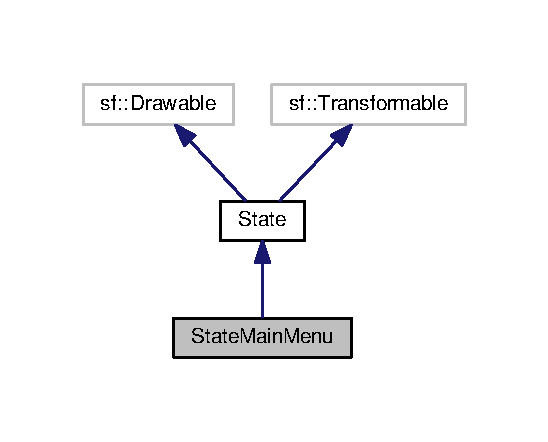
\includegraphics[width=263pt]{class_state_main_menu__inherit__graph}
\end{center}
\end{figure}


Collaboration diagram for State\+Main\+Menu\+:
\nopagebreak
\begin{figure}[H]
\begin{center}
\leavevmode
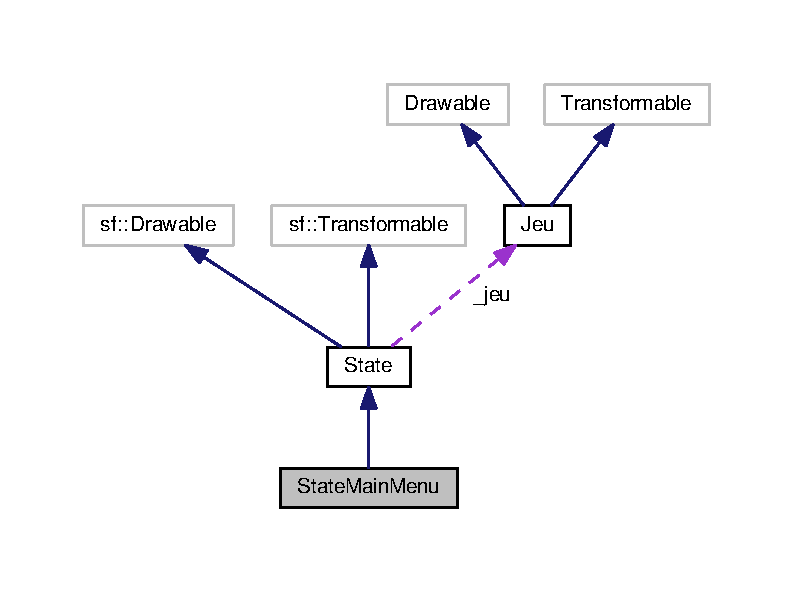
\includegraphics[width=350pt]{class_state_main_menu__coll__graph}
\end{center}
\end{figure}
\subsection*{Public Member Functions}
\begin{DoxyCompactItemize}
\item 
\hyperlink{class_state_main_menu_ad1dfd37dfda1c880599b8a51be5f55cd}{State\+Main\+Menu} (\hyperlink{class_jeu}{Jeu} $\ast$jeu)
\begin{DoxyCompactList}\small\item\em Constructeur. \end{DoxyCompactList}\item 
\hyperlink{class_state_main_menu_aae1ad451be64082e6e8f021d72d2050c}{$\sim$\+State\+Main\+Menu} ()
\begin{DoxyCompactList}\small\item\em Destructeur. \end{DoxyCompactList}\item 
virtual void \hyperlink{class_state_main_menu_ae372daf9ed9b53da4c23c01d4a7787a4}{draw} (sf\+::\+Render\+Target \&target, sf\+::\+Render\+States states) const 
\begin{DoxyCompactList}\small\item\em Dessine le menu. \end{DoxyCompactList}\item 
virtual void \hyperlink{class_state_main_menu_a714cb2def73b1146ad862e667b6996ee}{press\+Up} ()
\begin{DoxyCompactList}\small\item\em Action à effectuer quand la touche Haut est appuyé \end{DoxyCompactList}\item 
virtual void \hyperlink{class_state_main_menu_a90c547b9d2aae731a752c71fb7c0ab4a}{press\+Down} ()
\begin{DoxyCompactList}\small\item\em Action à effectuer quand la touche Bas est appuyé \end{DoxyCompactList}\item 
virtual void \hyperlink{class_state_main_menu_a25dac2e7223f8f36a9e4f372bb25b702}{press\+Enter} ()
\begin{DoxyCompactList}\small\item\em Action à effectuer quand Entrée est appuyé \end{DoxyCompactList}\end{DoxyCompactItemize}
\subsection*{Additional Inherited Members}


\subsection{Detailed Description}
Etat Main\+Menu rattaché au Pattern \hyperlink{class_state}{State}. 

\hyperlink{class_state_main_menu}{State\+Main\+Menu} 

\subsection{Constructor \& Destructor Documentation}
\hypertarget{class_state_main_menu_ad1dfd37dfda1c880599b8a51be5f55cd}{\index{State\+Main\+Menu@{State\+Main\+Menu}!State\+Main\+Menu@{State\+Main\+Menu}}
\index{State\+Main\+Menu@{State\+Main\+Menu}!State\+Main\+Menu@{State\+Main\+Menu}}
\subsubsection[{State\+Main\+Menu}]{\setlength{\rightskip}{0pt plus 5cm}State\+Main\+Menu\+::\+State\+Main\+Menu (
\begin{DoxyParamCaption}
\item[{{\bf Jeu} $\ast$}]{jeu}
\end{DoxyParamCaption}
)}}\label{class_state_main_menu_ad1dfd37dfda1c880599b8a51be5f55cd}


Constructeur. 

Constructeur de la classe \hyperlink{class_state_main_menu}{State\+Main\+Menu}


\begin{DoxyParams}{Parameters}
{\em jeu} & \+: jeu sur lequel s'applique le menu \\
\hline
\end{DoxyParams}
\hypertarget{class_state_main_menu_aae1ad451be64082e6e8f021d72d2050c}{\index{State\+Main\+Menu@{State\+Main\+Menu}!````~State\+Main\+Menu@{$\sim$\+State\+Main\+Menu}}
\index{````~State\+Main\+Menu@{$\sim$\+State\+Main\+Menu}!State\+Main\+Menu@{State\+Main\+Menu}}
\subsubsection[{$\sim$\+State\+Main\+Menu}]{\setlength{\rightskip}{0pt plus 5cm}State\+Main\+Menu\+::$\sim$\+State\+Main\+Menu (
\begin{DoxyParamCaption}
{}
\end{DoxyParamCaption}
)}}\label{class_state_main_menu_aae1ad451be64082e6e8f021d72d2050c}


Destructeur. 

Destructeur de la classe \hyperlink{class_state_main_menu}{State\+Main\+Menu} 

\subsection{Member Function Documentation}
\hypertarget{class_state_main_menu_ae372daf9ed9b53da4c23c01d4a7787a4}{\index{State\+Main\+Menu@{State\+Main\+Menu}!draw@{draw}}
\index{draw@{draw}!State\+Main\+Menu@{State\+Main\+Menu}}
\subsubsection[{draw}]{\setlength{\rightskip}{0pt plus 5cm}void State\+Main\+Menu\+::draw (
\begin{DoxyParamCaption}
\item[{sf\+::\+Render\+Target \&}]{target, }
\item[{sf\+::\+Render\+States}]{states}
\end{DoxyParamCaption}
) const\hspace{0.3cm}{\ttfamily [virtual]}}}\label{class_state_main_menu_ae372daf9ed9b53da4c23c01d4a7787a4}


Dessine le menu. 

Dessine le menu principal


\begin{DoxyParams}{Parameters}
{\em target} & \+: objet à dessiner, states \+: applique la transformation (S\+F\+M\+L Function) \\
\hline
\end{DoxyParams}


Implements \hyperlink{class_state_a7e115388c37a05ee165a395f3119d685}{State}.

\hypertarget{class_state_main_menu_a90c547b9d2aae731a752c71fb7c0ab4a}{\index{State\+Main\+Menu@{State\+Main\+Menu}!press\+Down@{press\+Down}}
\index{press\+Down@{press\+Down}!State\+Main\+Menu@{State\+Main\+Menu}}
\subsubsection[{press\+Down}]{\setlength{\rightskip}{0pt plus 5cm}void State\+Main\+Menu\+::press\+Down (
\begin{DoxyParamCaption}
{}
\end{DoxyParamCaption}
)\hspace{0.3cm}{\ttfamily [virtual]}}}\label{class_state_main_menu_a90c547b9d2aae731a752c71fb7c0ab4a}


Action à effectuer quand la touche Bas est appuyé 

Gère les actions rattachées à la touche Bas. 

Implements \hyperlink{class_state_a0f77b5ab3a8cbdd35fef9d0d5b414e1f}{State}.

\hypertarget{class_state_main_menu_a25dac2e7223f8f36a9e4f372bb25b702}{\index{State\+Main\+Menu@{State\+Main\+Menu}!press\+Enter@{press\+Enter}}
\index{press\+Enter@{press\+Enter}!State\+Main\+Menu@{State\+Main\+Menu}}
\subsubsection[{press\+Enter}]{\setlength{\rightskip}{0pt plus 5cm}void State\+Main\+Menu\+::press\+Enter (
\begin{DoxyParamCaption}
{}
\end{DoxyParamCaption}
)\hspace{0.3cm}{\ttfamily [virtual]}}}\label{class_state_main_menu_a25dac2e7223f8f36a9e4f372bb25b702}


Action à effectuer quand Entrée est appuyé 

Gère les actions rattachées à la touhce Entrée. 

Reimplemented from \hyperlink{class_state_a62d60bde66bc403c40ece17e069a616d}{State}.

\hypertarget{class_state_main_menu_a714cb2def73b1146ad862e667b6996ee}{\index{State\+Main\+Menu@{State\+Main\+Menu}!press\+Up@{press\+Up}}
\index{press\+Up@{press\+Up}!State\+Main\+Menu@{State\+Main\+Menu}}
\subsubsection[{press\+Up}]{\setlength{\rightskip}{0pt plus 5cm}void State\+Main\+Menu\+::press\+Up (
\begin{DoxyParamCaption}
{}
\end{DoxyParamCaption}
)\hspace{0.3cm}{\ttfamily [virtual]}}}\label{class_state_main_menu_a714cb2def73b1146ad862e667b6996ee}


Action à effectuer quand la touche Haut est appuyé 

Gère les actions rattachées à la touche Haut. 

Implements \hyperlink{class_state_ab3837b57093899dbdb323540c75a79e8}{State}.



The documentation for this class was generated from the following file\+:\begin{DoxyCompactItemize}
\item 
\hyperlink{_state_main_menu_8hpp}{State\+Main\+Menu.\+hpp}\end{DoxyCompactItemize}

\hypertarget{class_state_stats}{\section{State\+Stats Class Reference}
\label{class_state_stats}\index{State\+Stats@{State\+Stats}}
}


Etat \hyperlink{class_state_stats}{State\+Stats} rattaché au Pattern \hyperlink{class_state}{State}.  




{\ttfamily \#include $<$State\+Stats.\+hpp$>$}



Inheritance diagram for State\+Stats\+:
\nopagebreak
\begin{figure}[H]
\begin{center}
\leavevmode
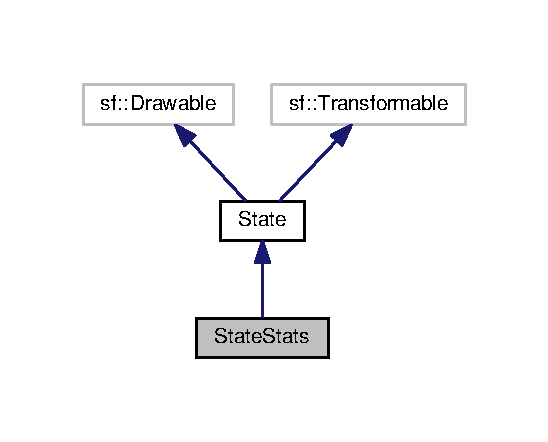
\includegraphics[width=263pt]{class_state_stats__inherit__graph}
\end{center}
\end{figure}


Collaboration diagram for State\+Stats\+:
\nopagebreak
\begin{figure}[H]
\begin{center}
\leavevmode
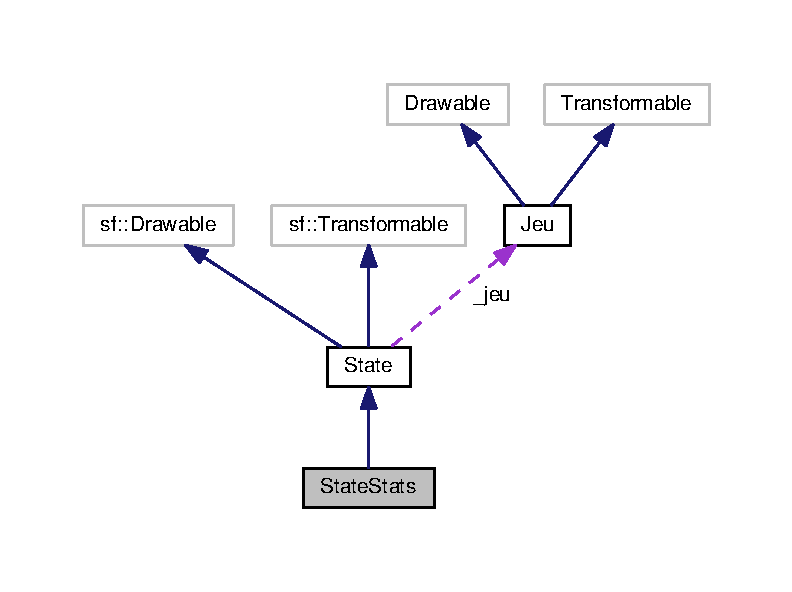
\includegraphics[width=350pt]{class_state_stats__coll__graph}
\end{center}
\end{figure}
\subsection*{Public Member Functions}
\begin{DoxyCompactItemize}
\item 
\hyperlink{class_state_stats_a01c0e31ffe6a1b8d9af8ca9c752fd29d}{State\+Stats} (\hyperlink{class_jeu}{Jeu} $\ast$jeu, \hyperlink{class_personnage}{Personnage} \&p)
\begin{DoxyCompactList}\small\item\em Constructeur. \end{DoxyCompactList}\item 
\hyperlink{class_state_stats_a1af5ae0229dfffd6586a54165c6af8b3}{$\sim$\+State\+Stats} ()
\begin{DoxyCompactList}\small\item\em Destrcuteur. \end{DoxyCompactList}\item 
virtual void \hyperlink{class_state_stats_ae8ee0b50f030d3057b0635158c170715}{draw} (sf\+::\+Render\+Target \&target, sf\+::\+Render\+States states) const 
\begin{DoxyCompactList}\small\item\em Dessine le menu. \end{DoxyCompactList}\item 
virtual void \hyperlink{class_state_stats_a4fd39389aa2debf191b718dc750ccf8a}{press\+Up} ()
\begin{DoxyCompactList}\small\item\em Action à effectuer quand la touche Haut est appuyé \end{DoxyCompactList}\item 
virtual void \hyperlink{class_state_stats_ac19acb64e561b57a02a826328aa827f6}{press\+Down} ()
\begin{DoxyCompactList}\small\item\em Action à effectuer quand la touche Bas est appuyé \end{DoxyCompactList}\item 
virtual void \hyperlink{class_state_stats_a12a42d0bc1a2d43c48d76fe9e1e0fdfd}{press\+Enter} ()
\begin{DoxyCompactList}\small\item\em Action à effectuer quand Entrée est appuyé \end{DoxyCompactList}\item 
void \hyperlink{class_state_stats_ad2d1de74b1ea43a077a3088861ad1b62}{set\+Is\+Level\+Finished} (bool Is\+Level\+Finished)
\begin{DoxyCompactList}\small\item\em Setter du bool Is\+Level\+Finished. \end{DoxyCompactList}\end{DoxyCompactItemize}
\subsection*{Additional Inherited Members}


\subsection{Detailed Description}
Etat \hyperlink{class_state_stats}{State\+Stats} rattaché au Pattern \hyperlink{class_state}{State}. 

\hyperlink{class_state_stats}{State\+Stats} 

\subsection{Constructor \& Destructor Documentation}
\hypertarget{class_state_stats_a01c0e31ffe6a1b8d9af8ca9c752fd29d}{\index{State\+Stats@{State\+Stats}!State\+Stats@{State\+Stats}}
\index{State\+Stats@{State\+Stats}!State\+Stats@{State\+Stats}}
\subsubsection[{State\+Stats}]{\setlength{\rightskip}{0pt plus 5cm}State\+Stats\+::\+State\+Stats (
\begin{DoxyParamCaption}
\item[{{\bf Jeu} $\ast$}]{jeu, }
\item[{{\bf Personnage} \&}]{p}
\end{DoxyParamCaption}
)}}\label{class_state_stats_a01c0e31ffe6a1b8d9af8ca9c752fd29d}


Constructeur. 

Constructeur de la classe \hyperlink{class_state_stats}{State\+Stats}


\begin{DoxyParams}{Parameters}
{\em jeu} & \+: jeu sur lequel on applique les stats, p \+: personnage sur lequel les stats sont enregistrés \\
\hline
\end{DoxyParams}
\hypertarget{class_state_stats_a1af5ae0229dfffd6586a54165c6af8b3}{\index{State\+Stats@{State\+Stats}!````~State\+Stats@{$\sim$\+State\+Stats}}
\index{````~State\+Stats@{$\sim$\+State\+Stats}!State\+Stats@{State\+Stats}}
\subsubsection[{$\sim$\+State\+Stats}]{\setlength{\rightskip}{0pt plus 5cm}State\+Stats\+::$\sim$\+State\+Stats (
\begin{DoxyParamCaption}
{}
\end{DoxyParamCaption}
)}}\label{class_state_stats_a1af5ae0229dfffd6586a54165c6af8b3}


Destrcuteur. 

Destructeur de la classe \hyperlink{class_state_stats}{State\+Stats} 

\subsection{Member Function Documentation}
\hypertarget{class_state_stats_ae8ee0b50f030d3057b0635158c170715}{\index{State\+Stats@{State\+Stats}!draw@{draw}}
\index{draw@{draw}!State\+Stats@{State\+Stats}}
\subsubsection[{draw}]{\setlength{\rightskip}{0pt plus 5cm}void State\+Stats\+::draw (
\begin{DoxyParamCaption}
\item[{sf\+::\+Render\+Target \&}]{target, }
\item[{sf\+::\+Render\+States}]{states}
\end{DoxyParamCaption}
) const\hspace{0.3cm}{\ttfamily [virtual]}}}\label{class_state_stats_ae8ee0b50f030d3057b0635158c170715}


Dessine le menu. 

Dessine le menu des stats


\begin{DoxyParams}{Parameters}
{\em target} & \+: objet à dessiner, states \+: applique la transformation (S\+F\+M\+L Function) \\
\hline
\end{DoxyParams}


Implements \hyperlink{class_state_a7e115388c37a05ee165a395f3119d685}{State}.

\hypertarget{class_state_stats_ac19acb64e561b57a02a826328aa827f6}{\index{State\+Stats@{State\+Stats}!press\+Down@{press\+Down}}
\index{press\+Down@{press\+Down}!State\+Stats@{State\+Stats}}
\subsubsection[{press\+Down}]{\setlength{\rightskip}{0pt plus 5cm}void State\+Stats\+::press\+Down (
\begin{DoxyParamCaption}
{}
\end{DoxyParamCaption}
)\hspace{0.3cm}{\ttfamily [virtual]}}}\label{class_state_stats_ac19acb64e561b57a02a826328aa827f6}


Action à effectuer quand la touche Bas est appuyé 

Gère les actions rattachées à la touche Bas. 

Implements \hyperlink{class_state_a0f77b5ab3a8cbdd35fef9d0d5b414e1f}{State}.

\hypertarget{class_state_stats_a12a42d0bc1a2d43c48d76fe9e1e0fdfd}{\index{State\+Stats@{State\+Stats}!press\+Enter@{press\+Enter}}
\index{press\+Enter@{press\+Enter}!State\+Stats@{State\+Stats}}
\subsubsection[{press\+Enter}]{\setlength{\rightskip}{0pt plus 5cm}void State\+Stats\+::press\+Enter (
\begin{DoxyParamCaption}
{}
\end{DoxyParamCaption}
)\hspace{0.3cm}{\ttfamily [virtual]}}}\label{class_state_stats_a12a42d0bc1a2d43c48d76fe9e1e0fdfd}


Action à effectuer quand Entrée est appuyé 

Gère les actions rattachées à la touhce Entrée. 

Reimplemented from \hyperlink{class_state_a62d60bde66bc403c40ece17e069a616d}{State}.

\hypertarget{class_state_stats_a4fd39389aa2debf191b718dc750ccf8a}{\index{State\+Stats@{State\+Stats}!press\+Up@{press\+Up}}
\index{press\+Up@{press\+Up}!State\+Stats@{State\+Stats}}
\subsubsection[{press\+Up}]{\setlength{\rightskip}{0pt plus 5cm}void State\+Stats\+::press\+Up (
\begin{DoxyParamCaption}
{}
\end{DoxyParamCaption}
)\hspace{0.3cm}{\ttfamily [virtual]}}}\label{class_state_stats_a4fd39389aa2debf191b718dc750ccf8a}


Action à effectuer quand la touche Haut est appuyé 

Gère les actions rattachées à la touche Haut. 

Implements \hyperlink{class_state_ab3837b57093899dbdb323540c75a79e8}{State}.

\hypertarget{class_state_stats_ad2d1de74b1ea43a077a3088861ad1b62}{\index{State\+Stats@{State\+Stats}!set\+Is\+Level\+Finished@{set\+Is\+Level\+Finished}}
\index{set\+Is\+Level\+Finished@{set\+Is\+Level\+Finished}!State\+Stats@{State\+Stats}}
\subsubsection[{set\+Is\+Level\+Finished}]{\setlength{\rightskip}{0pt plus 5cm}void State\+Stats\+::set\+Is\+Level\+Finished (
\begin{DoxyParamCaption}
\item[{bool}]{Is\+Level\+Finished}
\end{DoxyParamCaption}
)}}\label{class_state_stats_ad2d1de74b1ea43a077a3088861ad1b62}


Setter du bool Is\+Level\+Finished. 

Setter pour le bool de fin de partie


\begin{DoxyParams}{Parameters}
{\em Is\+Level\+Finished} & \+: valeur qui remplacera l'ancienne \\
\hline
\end{DoxyParams}


The documentation for this class was generated from the following file\+:\begin{DoxyCompactItemize}
\item 
\hyperlink{_state_stats_8hpp}{State\+Stats.\+hpp}\end{DoxyCompactItemize}

\hypertarget{class_tile_map}{\section{Tile\+Map Class Reference}
\label{class_tile_map}\index{Tile\+Map@{Tile\+Map}}
}


Classe définissant un map.  




{\ttfamily \#include $<$Tile\+Map.\+hpp$>$}



Inheritance diagram for Tile\+Map\+:
\nopagebreak
\begin{figure}[H]
\begin{center}
\leavevmode
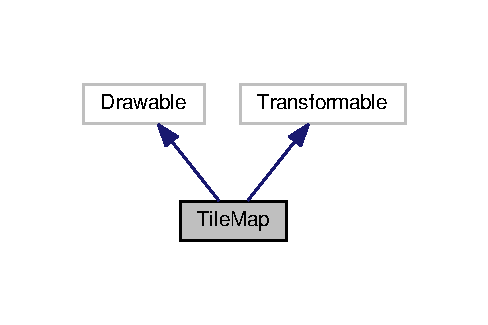
\includegraphics[width=234pt]{class_tile_map__inherit__graph}
\end{center}
\end{figure}


Collaboration diagram for Tile\+Map\+:
\nopagebreak
\begin{figure}[H]
\begin{center}
\leavevmode
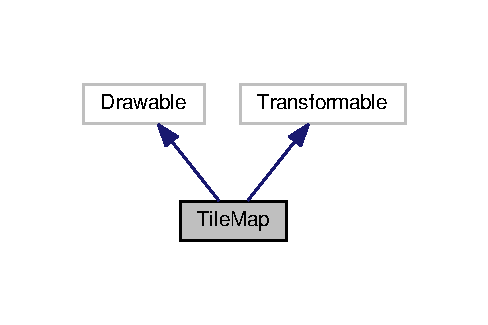
\includegraphics[width=234pt]{class_tile_map__coll__graph}
\end{center}
\end{figure}
\subsection*{Public Member Functions}
\begin{DoxyCompactItemize}
\item 
\hyperlink{class_tile_map_a20b74c68d508aefc556237ca98b6d84f}{Tile\+Map} (std\+::string niveau, sf\+::\+Vector2f \&gravity, const \hyperlink{class_personnage}{Personnage} \&p)
\begin{DoxyCompactList}\small\item\em Constructeur. \end{DoxyCompactList}\item 
\hyperlink{class_tile_map_a3448728e45d6a43fff3a02d4c6d72e9d}{$\sim$\+Tile\+Map} ()
\begin{DoxyCompactList}\small\item\em Destrcuteur. \end{DoxyCompactList}\item 
bool \hyperlink{class_tile_map_a5126cb10237b3d0c0c9cbcf4dca849ac}{load} (const std\+::string \&tileset, sf\+::\+Vector2u tile\+Size)
\begin{DoxyCompactList}\small\item\em charge le niveau avec la texture de la tileset \end{DoxyCompactList}\item 
bool \hyperlink{class_tile_map_a2dc99a84ead7dac1481375144a990412}{collision} (const sf\+::\+Vector2f \&point, const sf\+::\+Vector2f \&vect) const 
\begin{DoxyCompactList}\small\item\em Vérifie la collision entre un point affecté par un vector et la map. \end{DoxyCompactList}\item 
bool \hyperlink{class_tile_map_a543431b7e68211aad223ae8c7b1086c0}{collision\+Haut} (const \hyperlink{class_alive_entity}{Alive\+Entity} \&ae) const 
\begin{DoxyCompactList}\small\item\em Vérifie la collision sur le haut de l'\hyperlink{class_alive_entity}{Alive\+Entity}. \end{DoxyCompactList}\item 
bool \hyperlink{class_tile_map_af0255568dfc16a024d6107722860db36}{collision\+Bas} (const \hyperlink{class_alive_entity}{Alive\+Entity} \&ae) const 
\begin{DoxyCompactList}\small\item\em Vérifie la collision sur le bas de l'\hyperlink{class_alive_entity}{Alive\+Entity}. \end{DoxyCompactList}\item 
bool \hyperlink{class_tile_map_ae19adae862a47ff532ebd6360e6a117d}{collision\+Droite} (const \hyperlink{class_alive_entity}{Alive\+Entity} \&ae) const 
\begin{DoxyCompactList}\small\item\em Vérifie la collision sur la droite de l'\hyperlink{class_alive_entity}{Alive\+Entity}. \end{DoxyCompactList}\item 
bool \hyperlink{class_tile_map_a1a01bab917e287eef1b2dd2985accc83}{collision\+Gauche} (const \hyperlink{class_alive_entity}{Alive\+Entity} \&ae) const 
\begin{DoxyCompactList}\small\item\em Vérifie la collision sur la gauche de l'\hyperlink{class_alive_entity}{Alive\+Entity}. \end{DoxyCompactList}\item 
unsigned int \hyperlink{class_tile_map_aad3bfcbf9997269b7af18e6cd66a83d3}{get\+Width} () const 
\begin{DoxyCompactList}\small\item\em Getter de Width. \end{DoxyCompactList}\item 
unsigned int \hyperlink{class_tile_map_aae7430209eb0f15d7a0d0476e2337c72}{get\+Height} () const 
\begin{DoxyCompactList}\small\item\em Getter de Height. \end{DoxyCompactList}\item 
sf\+::\+Vector2f \hyperlink{class_tile_map_a2d2cdb4a85f60bee4204c0163c29b7cd}{get\+Gravity} () const 
\begin{DoxyCompactList}\small\item\em Getter de la Gravité \end{DoxyCompactList}\item 
sf\+::\+Vector2f \hyperlink{class_tile_map_ab91140b620ac86fcce9649b385e1132f}{get\+Spawn} () const 
\begin{DoxyCompactList}\small\item\em Getter des coordonnées de spawn. \end{DoxyCompactList}\item 
sf\+::\+Rectangle\+Shape $\ast$ \hyperlink{class_tile_map_a9f0637a3a0afea5f28e846f11f22f6cf}{get\+Level\+End} ()
\begin{DoxyCompactList}\small\item\em Getter de la fin du niveau. \end{DoxyCompactList}\item 
std\+::string \hyperlink{class_tile_map_ab498153694e7a79853fc6fb2a10887ad}{get\+Level\+Name} () const 
\begin{DoxyCompactList}\small\item\em Getter du nom du niveau. \end{DoxyCompactList}\item 
std\+::vector$<$ \hyperlink{class_enemy}{Enemy} $\ast$ $>$ \hyperlink{class_tile_map_a67f641da59fdaab20da87bcca89a1038}{get\+Enemies} ()
\begin{DoxyCompactList}\small\item\em Getter des ennemis. \end{DoxyCompactList}\item 
unsigned int \hyperlink{class_tile_map_a72d2f2c89b9521d8632a724b246f6e43}{next\+Tile\+Y} (float x) const 
\begin{DoxyCompactList}\small\item\em Retourne la tuile suivante. \end{DoxyCompactList}\item 
unsigned int \hyperlink{class_tile_map_acca5310b644c02342e0d4829a887d1e7}{previous\+Tile\+Y} (float x) const 
\begin{DoxyCompactList}\small\item\em Retourne la tuile précédante. \end{DoxyCompactList}\item 
void \hyperlink{class_tile_map_a5ee6a66152cf4a52f3232369ac19132f}{reset} ()
\begin{DoxyCompactList}\small\item\em Réinitialise la map. \end{DoxyCompactList}\item 
void \hyperlink{class_tile_map_acf30f34bdb6d18a36db9f1e682afc1a9}{change\+Position\+X} (float gap)
\begin{DoxyCompactList}\small\item\em Décale tout les objets de la \hyperlink{class_tile_map}{Tile\+Map}. \end{DoxyCompactList}\item 
void \hyperlink{class_tile_map_a275b065e4d410f5649b4fcbddbdeae7b}{change\+Position\+Y} (float gap)
\begin{DoxyCompactList}\small\item\em Décale tout les objets de la \hyperlink{class_tile_map}{Tile\+Map}. \end{DoxyCompactList}\item 
void \hyperlink{class_tile_map_a2418329f152f039cf32b060ad4e0db55}{kill\+Enemy} (\hyperlink{class_enemy}{Enemy} $\ast$e)
\begin{DoxyCompactList}\small\item\em Supprime l'\hyperlink{class_enemy}{Enemy} tué \end{DoxyCompactList}\item 
void \hyperlink{class_tile_map_ad813990bc076f44b52ccafd5495df116}{add\+Enemy} (\hyperlink{class_enemy}{Enemy} $\ast$e)
\begin{DoxyCompactList}\small\item\em Ajoute un enemy au niveau. \end{DoxyCompactList}\end{DoxyCompactItemize}


\subsection{Detailed Description}
Classe définissant un map. 

\subsection{Constructor \& Destructor Documentation}
\hypertarget{class_tile_map_a20b74c68d508aefc556237ca98b6d84f}{\index{Tile\+Map@{Tile\+Map}!Tile\+Map@{Tile\+Map}}
\index{Tile\+Map@{Tile\+Map}!Tile\+Map@{Tile\+Map}}
\subsubsection[{Tile\+Map}]{\setlength{\rightskip}{0pt plus 5cm}Tile\+Map\+::\+Tile\+Map (
\begin{DoxyParamCaption}
\item[{std\+::string}]{niveau, }
\item[{sf\+::\+Vector2f \&}]{gravity, }
\item[{const {\bf Personnage} \&}]{p}
\end{DoxyParamCaption}
)}}\label{class_tile_map_a20b74c68d508aefc556237ca98b6d84f}


Constructeur. 

Constructeur de la classe \hyperlink{class_tile_map}{Tile\+Map}


\begin{DoxyParams}{Parameters}
{\em niveau} & \+: string définissant le niveau par des tuiles, gravity \+: Vecteur 2\+D initialisant la gravité. \\
\hline
\end{DoxyParams}
\hypertarget{class_tile_map_a3448728e45d6a43fff3a02d4c6d72e9d}{\index{Tile\+Map@{Tile\+Map}!````~Tile\+Map@{$\sim$\+Tile\+Map}}
\index{````~Tile\+Map@{$\sim$\+Tile\+Map}!Tile\+Map@{Tile\+Map}}
\subsubsection[{$\sim$\+Tile\+Map}]{\setlength{\rightskip}{0pt plus 5cm}Tile\+Map\+::$\sim$\+Tile\+Map (
\begin{DoxyParamCaption}
{}
\end{DoxyParamCaption}
)}}\label{class_tile_map_a3448728e45d6a43fff3a02d4c6d72e9d}


Destrcuteur. 

Destructeur de la classe \hyperlink{class_tile_map}{Tile\+Map} 

\subsection{Member Function Documentation}
\hypertarget{class_tile_map_ad813990bc076f44b52ccafd5495df116}{\index{Tile\+Map@{Tile\+Map}!add\+Enemy@{add\+Enemy}}
\index{add\+Enemy@{add\+Enemy}!Tile\+Map@{Tile\+Map}}
\subsubsection[{add\+Enemy}]{\setlength{\rightskip}{0pt plus 5cm}void Tile\+Map\+::add\+Enemy (
\begin{DoxyParamCaption}
\item[{{\bf Enemy} $\ast$}]{e}
\end{DoxyParamCaption}
)}}\label{class_tile_map_ad813990bc076f44b52ccafd5495df116}


Ajoute un enemy au niveau. 

Ajoute un enemy au niveau


\begin{DoxyParams}{Parameters}
{\em e} & L'ennemi à ajouter \\
\hline
\end{DoxyParams}
\hypertarget{class_tile_map_acf30f34bdb6d18a36db9f1e682afc1a9}{\index{Tile\+Map@{Tile\+Map}!change\+Position\+X@{change\+Position\+X}}
\index{change\+Position\+X@{change\+Position\+X}!Tile\+Map@{Tile\+Map}}
\subsubsection[{change\+Position\+X}]{\setlength{\rightskip}{0pt plus 5cm}void Tile\+Map\+::change\+Position\+X (
\begin{DoxyParamCaption}
\item[{float}]{gap}
\end{DoxyParamCaption}
)}}\label{class_tile_map_acf30f34bdb6d18a36db9f1e682afc1a9}


Décale tout les objets de la \hyperlink{class_tile_map}{Tile\+Map}. 

Décale tout de gap pixels en X


\begin{DoxyParams}{Parameters}
{\em gap} & \+: valeur du décalage \\
\hline
\end{DoxyParams}
\hypertarget{class_tile_map_a275b065e4d410f5649b4fcbddbdeae7b}{\index{Tile\+Map@{Tile\+Map}!change\+Position\+Y@{change\+Position\+Y}}
\index{change\+Position\+Y@{change\+Position\+Y}!Tile\+Map@{Tile\+Map}}
\subsubsection[{change\+Position\+Y}]{\setlength{\rightskip}{0pt plus 5cm}void Tile\+Map\+::change\+Position\+Y (
\begin{DoxyParamCaption}
\item[{float}]{gap}
\end{DoxyParamCaption}
)}}\label{class_tile_map_a275b065e4d410f5649b4fcbddbdeae7b}


Décale tout les objets de la \hyperlink{class_tile_map}{Tile\+Map}. 

Décale tout de gap pixels en Y


\begin{DoxyParams}{Parameters}
{\em gap} & \+: valeur du décalage \\
\hline
\end{DoxyParams}
\hypertarget{class_tile_map_a2dc99a84ead7dac1481375144a990412}{\index{Tile\+Map@{Tile\+Map}!collision@{collision}}
\index{collision@{collision}!Tile\+Map@{Tile\+Map}}
\subsubsection[{collision}]{\setlength{\rightskip}{0pt plus 5cm}bool Tile\+Map\+::collision (
\begin{DoxyParamCaption}
\item[{const sf\+::\+Vector2f \&}]{point, }
\item[{const sf\+::\+Vector2f \&}]{vect}
\end{DoxyParamCaption}
) const}}\label{class_tile_map_a2dc99a84ead7dac1481375144a990412}


Vérifie la collision entre un point affecté par un vector et la map. 

Vérifie si le point est en collision avec la map après son déplacement


\begin{DoxyParams}{Parameters}
{\em point} & \+: point à vérifier, vect \+: mouvement à appliquer pour la vérification \\
\hline
\end{DoxyParams}
\begin{DoxyReturn}{Returns}
Renvoi s'il y a une collision 
\end{DoxyReturn}
\hypertarget{class_tile_map_af0255568dfc16a024d6107722860db36}{\index{Tile\+Map@{Tile\+Map}!collision\+Bas@{collision\+Bas}}
\index{collision\+Bas@{collision\+Bas}!Tile\+Map@{Tile\+Map}}
\subsubsection[{collision\+Bas}]{\setlength{\rightskip}{0pt plus 5cm}bool Tile\+Map\+::collision\+Bas (
\begin{DoxyParamCaption}
\item[{const {\bf Alive\+Entity} \&}]{ae}
\end{DoxyParamCaption}
) const}}\label{class_tile_map_af0255568dfc16a024d6107722860db36}


Vérifie la collision sur le bas de l'\hyperlink{class_alive_entity}{Alive\+Entity}. 

Vérifie si une collision existe entre le bas du paramètre et la map


\begin{DoxyParams}{Parameters}
{\em ae} & \+: objet à vérifier \\
\hline
\end{DoxyParams}
\begin{DoxyReturn}{Returns}
L'état de la collision 
\end{DoxyReturn}
\hypertarget{class_tile_map_ae19adae862a47ff532ebd6360e6a117d}{\index{Tile\+Map@{Tile\+Map}!collision\+Droite@{collision\+Droite}}
\index{collision\+Droite@{collision\+Droite}!Tile\+Map@{Tile\+Map}}
\subsubsection[{collision\+Droite}]{\setlength{\rightskip}{0pt plus 5cm}bool Tile\+Map\+::collision\+Droite (
\begin{DoxyParamCaption}
\item[{const {\bf Alive\+Entity} \&}]{ae}
\end{DoxyParamCaption}
) const}}\label{class_tile_map_ae19adae862a47ff532ebd6360e6a117d}


Vérifie la collision sur la droite de l'\hyperlink{class_alive_entity}{Alive\+Entity}. 

Vérifie si une collision existe entre la droite du paramètre et la map


\begin{DoxyParams}{Parameters}
{\em ae} & \+: objet à vérifier \\
\hline
\end{DoxyParams}
\begin{DoxyReturn}{Returns}
L'état de la collision 
\end{DoxyReturn}
\hypertarget{class_tile_map_a1a01bab917e287eef1b2dd2985accc83}{\index{Tile\+Map@{Tile\+Map}!collision\+Gauche@{collision\+Gauche}}
\index{collision\+Gauche@{collision\+Gauche}!Tile\+Map@{Tile\+Map}}
\subsubsection[{collision\+Gauche}]{\setlength{\rightskip}{0pt plus 5cm}bool Tile\+Map\+::collision\+Gauche (
\begin{DoxyParamCaption}
\item[{const {\bf Alive\+Entity} \&}]{ae}
\end{DoxyParamCaption}
) const}}\label{class_tile_map_a1a01bab917e287eef1b2dd2985accc83}


Vérifie la collision sur la gauche de l'\hyperlink{class_alive_entity}{Alive\+Entity}. 

Vérifie si une collision existe entre la gauche du paramètre et la map


\begin{DoxyParams}{Parameters}
{\em ae} & \+: objet à vérifier \\
\hline
\end{DoxyParams}
\begin{DoxyReturn}{Returns}
L'état de la collision 
\end{DoxyReturn}
\hypertarget{class_tile_map_a543431b7e68211aad223ae8c7b1086c0}{\index{Tile\+Map@{Tile\+Map}!collision\+Haut@{collision\+Haut}}
\index{collision\+Haut@{collision\+Haut}!Tile\+Map@{Tile\+Map}}
\subsubsection[{collision\+Haut}]{\setlength{\rightskip}{0pt plus 5cm}bool Tile\+Map\+::collision\+Haut (
\begin{DoxyParamCaption}
\item[{const {\bf Alive\+Entity} \&}]{ae}
\end{DoxyParamCaption}
) const}}\label{class_tile_map_a543431b7e68211aad223ae8c7b1086c0}


Vérifie la collision sur le haut de l'\hyperlink{class_alive_entity}{Alive\+Entity}. 

Vérifie si une collision existe entre le haut du paramètre et la map


\begin{DoxyParams}{Parameters}
{\em ae} & \+: objet à vérifier \\
\hline
\end{DoxyParams}
\begin{DoxyReturn}{Returns}
L'état de la collision 
\end{DoxyReturn}
\hypertarget{class_tile_map_a67f641da59fdaab20da87bcca89a1038}{\index{Tile\+Map@{Tile\+Map}!get\+Enemies@{get\+Enemies}}
\index{get\+Enemies@{get\+Enemies}!Tile\+Map@{Tile\+Map}}
\subsubsection[{get\+Enemies}]{\setlength{\rightskip}{0pt plus 5cm}std\+::vector$<$ {\bf Enemy} $\ast$ $>$ Tile\+Map\+::get\+Enemies (
\begin{DoxyParamCaption}
{}
\end{DoxyParamCaption}
)}}\label{class_tile_map_a67f641da59fdaab20da87bcca89a1038}


Getter des ennemis. 

Récupère un vector contenant la liste de tout les ennemis de la \hyperlink{class_tile_map}{Tile\+Map}

\begin{DoxyReturn}{Returns}
La liste des ennemis de la map 
\end{DoxyReturn}
\hypertarget{class_tile_map_a2d2cdb4a85f60bee4204c0163c29b7cd}{\index{Tile\+Map@{Tile\+Map}!get\+Gravity@{get\+Gravity}}
\index{get\+Gravity@{get\+Gravity}!Tile\+Map@{Tile\+Map}}
\subsubsection[{get\+Gravity}]{\setlength{\rightskip}{0pt plus 5cm}sf\+::\+Vector2f Tile\+Map\+::get\+Gravity (
\begin{DoxyParamCaption}
{}
\end{DoxyParamCaption}
) const}}\label{class_tile_map_a2d2cdb4a85f60bee4204c0163c29b7cd}


Getter de la Gravité 

Retourne la valeur (2\+D) de la gravité.

\begin{DoxyReturn}{Returns}
Un Vector2f de la Gravité. 
\end{DoxyReturn}
\hypertarget{class_tile_map_aae7430209eb0f15d7a0d0476e2337c72}{\index{Tile\+Map@{Tile\+Map}!get\+Height@{get\+Height}}
\index{get\+Height@{get\+Height}!Tile\+Map@{Tile\+Map}}
\subsubsection[{get\+Height}]{\setlength{\rightskip}{0pt plus 5cm}unsigned int Tile\+Map\+::get\+Height (
\begin{DoxyParamCaption}
{}
\end{DoxyParamCaption}
) const}}\label{class_tile_map_aae7430209eb0f15d7a0d0476e2337c72}


Getter de Height. 

Retourne la hauteur du Level.

\begin{DoxyReturn}{Returns}
La hauteur du Level. 
\end{DoxyReturn}
\hypertarget{class_tile_map_a9f0637a3a0afea5f28e846f11f22f6cf}{\index{Tile\+Map@{Tile\+Map}!get\+Level\+End@{get\+Level\+End}}
\index{get\+Level\+End@{get\+Level\+End}!Tile\+Map@{Tile\+Map}}
\subsubsection[{get\+Level\+End}]{\setlength{\rightskip}{0pt plus 5cm}sf\+::\+Rectangle\+Shape $\ast$ Tile\+Map\+::get\+Level\+End (
\begin{DoxyParamCaption}
{}
\end{DoxyParamCaption}
)}}\label{class_tile_map_a9f0637a3a0afea5f28e846f11f22f6cf}


Getter de la fin du niveau. 

Récupère la Rectangle\+Shape du bloc de fin de niveau

\begin{DoxyReturn}{Returns}
La Rectangle\+Shape de fin de niveau 
\end{DoxyReturn}
\hypertarget{class_tile_map_ab498153694e7a79853fc6fb2a10887ad}{\index{Tile\+Map@{Tile\+Map}!get\+Level\+Name@{get\+Level\+Name}}
\index{get\+Level\+Name@{get\+Level\+Name}!Tile\+Map@{Tile\+Map}}
\subsubsection[{get\+Level\+Name}]{\setlength{\rightskip}{0pt plus 5cm}std\+::string Tile\+Map\+::get\+Level\+Name (
\begin{DoxyParamCaption}
{}
\end{DoxyParamCaption}
) const}}\label{class_tile_map_ab498153694e7a79853fc6fb2a10887ad}


Getter du nom du niveau. 

Récupère le nom du niveau en cours

\begin{DoxyReturn}{Returns}
Le nom du niveau 
\end{DoxyReturn}
\hypertarget{class_tile_map_ab91140b620ac86fcce9649b385e1132f}{\index{Tile\+Map@{Tile\+Map}!get\+Spawn@{get\+Spawn}}
\index{get\+Spawn@{get\+Spawn}!Tile\+Map@{Tile\+Map}}
\subsubsection[{get\+Spawn}]{\setlength{\rightskip}{0pt plus 5cm}sf\+::\+Vector2f Tile\+Map\+::get\+Spawn (
\begin{DoxyParamCaption}
{}
\end{DoxyParamCaption}
) const}}\label{class_tile_map_ab91140b620ac86fcce9649b385e1132f}


Getter des coordonnées de spawn. 

\begin{DoxyReturn}{Returns}
Un Vector2f du spawn. 
\end{DoxyReturn}
\hypertarget{class_tile_map_aad3bfcbf9997269b7af18e6cd66a83d3}{\index{Tile\+Map@{Tile\+Map}!get\+Width@{get\+Width}}
\index{get\+Width@{get\+Width}!Tile\+Map@{Tile\+Map}}
\subsubsection[{get\+Width}]{\setlength{\rightskip}{0pt plus 5cm}unsigned int Tile\+Map\+::get\+Width (
\begin{DoxyParamCaption}
{}
\end{DoxyParamCaption}
) const}}\label{class_tile_map_aad3bfcbf9997269b7af18e6cd66a83d3}


Getter de Width. 

Retourne la largeur du Level.

\begin{DoxyReturn}{Returns}
La largeur du Level. 
\end{DoxyReturn}
\hypertarget{class_tile_map_a2418329f152f039cf32b060ad4e0db55}{\index{Tile\+Map@{Tile\+Map}!kill\+Enemy@{kill\+Enemy}}
\index{kill\+Enemy@{kill\+Enemy}!Tile\+Map@{Tile\+Map}}
\subsubsection[{kill\+Enemy}]{\setlength{\rightskip}{0pt plus 5cm}void Tile\+Map\+::kill\+Enemy (
\begin{DoxyParamCaption}
\item[{{\bf Enemy} $\ast$}]{e}
\end{DoxyParamCaption}
)}}\label{class_tile_map_a2418329f152f039cf32b060ad4e0db55}


Supprime l'\hyperlink{class_enemy}{Enemy} tué 

Supprime un ennemi lors de sa mort


\begin{DoxyParams}{Parameters}
{\em e} & \+: ennemi tué \\
\hline
\end{DoxyParams}
\hypertarget{class_tile_map_a5126cb10237b3d0c0c9cbcf4dca849ac}{\index{Tile\+Map@{Tile\+Map}!load@{load}}
\index{load@{load}!Tile\+Map@{Tile\+Map}}
\subsubsection[{load}]{\setlength{\rightskip}{0pt plus 5cm}bool Tile\+Map\+::load (
\begin{DoxyParamCaption}
\item[{const std\+::string \&}]{tileset, }
\item[{sf\+::\+Vector2u}]{tile\+Size}
\end{DoxyParamCaption}
)}}\label{class_tile_map_a5126cb10237b3d0c0c9cbcf4dca849ac}


charge le niveau avec la texture de la tileset 

Fonction chargeant le niveau, en utilisant comme texture la tileset prise en entrée.


\begin{DoxyParams}{Parameters}
{\em tileset} & \+: string contenant le nom du fichier contenant les tuiles, tile\+Size \+: taille des tuiles \\
\hline
\end{DoxyParams}
\hypertarget{class_tile_map_a72d2f2c89b9521d8632a724b246f6e43}{\index{Tile\+Map@{Tile\+Map}!next\+Tile\+Y@{next\+Tile\+Y}}
\index{next\+Tile\+Y@{next\+Tile\+Y}!Tile\+Map@{Tile\+Map}}
\subsubsection[{next\+Tile\+Y}]{\setlength{\rightskip}{0pt plus 5cm}unsigned int Tile\+Map\+::next\+Tile\+Y (
\begin{DoxyParamCaption}
\item[{float}]{x}
\end{DoxyParamCaption}
) const}}\label{class_tile_map_a72d2f2c89b9521d8632a724b246f6e43}


Retourne la tuile suivante. 

Renvoi le pixel ou commence la tuile suivant celle en parametre

\begin{DoxyReturn}{Returns}
La tuile suivante 
\end{DoxyReturn}
\hypertarget{class_tile_map_acca5310b644c02342e0d4829a887d1e7}{\index{Tile\+Map@{Tile\+Map}!previous\+Tile\+Y@{previous\+Tile\+Y}}
\index{previous\+Tile\+Y@{previous\+Tile\+Y}!Tile\+Map@{Tile\+Map}}
\subsubsection[{previous\+Tile\+Y}]{\setlength{\rightskip}{0pt plus 5cm}unsigned int Tile\+Map\+::previous\+Tile\+Y (
\begin{DoxyParamCaption}
\item[{float}]{x}
\end{DoxyParamCaption}
) const}}\label{class_tile_map_acca5310b644c02342e0d4829a887d1e7}


Retourne la tuile précédante. 

Renvoi le pixel ou commence la tuile précédant celle en parametre

\begin{DoxyReturn}{Returns}
La tuile précédante 
\end{DoxyReturn}
\hypertarget{class_tile_map_a5ee6a66152cf4a52f3232369ac19132f}{\index{Tile\+Map@{Tile\+Map}!reset@{reset}}
\index{reset@{reset}!Tile\+Map@{Tile\+Map}}
\subsubsection[{reset}]{\setlength{\rightskip}{0pt plus 5cm}void Tile\+Map\+::reset (
\begin{DoxyParamCaption}
{}
\end{DoxyParamCaption}
)}}\label{class_tile_map_a5ee6a66152cf4a52f3232369ac19132f}


Réinitialise la map. 

Supprime tout les ennemis et recharge le layer 

The documentation for this class was generated from the following file\+:\begin{DoxyCompactItemize}
\item 
\hyperlink{_tile_map_8hpp}{Tile\+Map.\+hpp}\end{DoxyCompactItemize}

\chapter{File Documentation}
\hypertarget{_a_i_8hpp}{\section{A\+I.\+hpp File Reference}
\label{_a_i_8hpp}\index{A\+I.\+hpp@{A\+I.\+hpp}}
}


Pattern Stratégie gérant les I\+A des ennemis.  


This graph shows which files directly or indirectly include this file\+:
\nopagebreak
\begin{figure}[H]
\begin{center}
\leavevmode
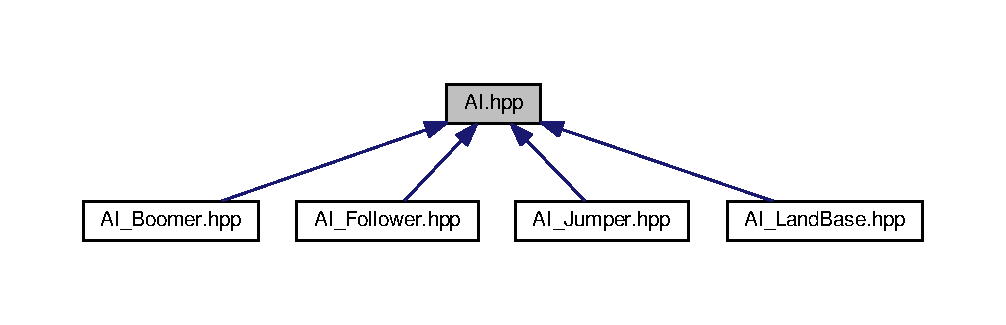
\includegraphics[width=350pt]{_a_i_8hpp__dep__incl}
\end{center}
\end{figure}
\subsection*{Classes}
\begin{DoxyCompactItemize}
\item 
class \hyperlink{class_a_i}{A\+I}
\begin{DoxyCompactList}\small\item\em Classe abstraites pour les I\+A des ennemis. \end{DoxyCompactList}\end{DoxyCompactItemize}


\subsection{Detailed Description}
Pattern Stratégie gérant les I\+A des ennemis. 

\begin{DoxyAuthor}{Author}
\{N. Guittonneau, P. Raballand\} 
\end{DoxyAuthor}
\begin{DoxyVersion}{Version}
1.\+0 
\end{DoxyVersion}
\begin{DoxyDate}{Date}
14/11/2015
\end{DoxyDate}
Gère les mouvements d'un \hyperlink{class_enemy}{Enemy} sur un map définit. 
\hypertarget{_a_i___boomer_8hpp}{\section{A\+I\+\_\+\+Boomer.\+hpp File Reference}
\label{_a_i___boomer_8hpp}\index{A\+I\+\_\+\+Boomer.\+hpp@{A\+I\+\_\+\+Boomer.\+hpp}}
}


\hyperlink{class_a_i}{A\+I} des boomers.  


{\ttfamily \#include $<$S\+F\+M\+L/\+Graphics.\+hpp$>$}\\*
{\ttfamily \#include \char`\"{}A\+I.\+hpp\char`\"{}}\\*
Include dependency graph for A\+I\+\_\+\+Boomer.\+hpp\+:
\nopagebreak
\begin{figure}[H]
\begin{center}
\leavevmode
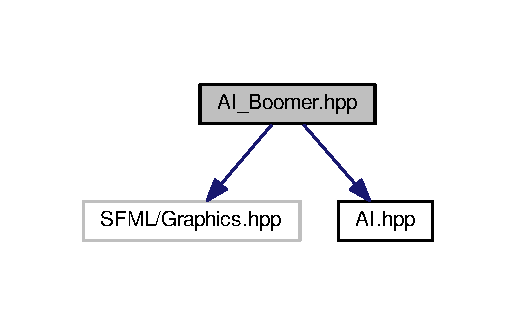
\includegraphics[width=247pt]{_a_i___boomer_8hpp__incl}
\end{center}
\end{figure}
\subsection*{Classes}
\begin{DoxyCompactItemize}
\item 
class \hyperlink{class_a_i___boomer}{A\+I\+\_\+\+Boomer}
\begin{DoxyCompactList}\small\item\em Classe gérant l'\hyperlink{class_a_i}{A\+I} des ennemi qui sautent. \end{DoxyCompactList}\end{DoxyCompactItemize}


\subsection{Detailed Description}
\hyperlink{class_a_i}{A\+I} des boomers. 

\begin{DoxyAuthor}{Author}
\{N. Guittonneau, P. Raballand\} 
\end{DoxyAuthor}
\begin{DoxyVersion}{Version}
1.\+0 
\end{DoxyVersion}
\begin{DoxyDate}{Date}
14/11/2015
\end{DoxyDate}
Gère les mouvement d'un \hyperlink{class_enemy}{Enemy} ayant pour base le mouvement de saut sur une \hyperlink{class_tile_map}{Tile\+Map} définie. Hérite du \hyperlink{class_a_i}{A\+I}. 
\hypertarget{_a_i___follower_8hpp}{\section{A\+I\+\_\+\+Follower.\+hpp File Reference}
\label{_a_i___follower_8hpp}\index{A\+I\+\_\+\+Follower.\+hpp@{A\+I\+\_\+\+Follower.\+hpp}}
}


\hyperlink{class_a_i}{A\+I} des enemy sautant.  


{\ttfamily \#include $<$S\+F\+M\+L/\+Graphics.\+hpp$>$}\\*
{\ttfamily \#include \char`\"{}A\+I.\+hpp\char`\"{}}\\*
Include dependency graph for A\+I\+\_\+\+Follower.\+hpp\+:
\nopagebreak
\begin{figure}[H]
\begin{center}
\leavevmode
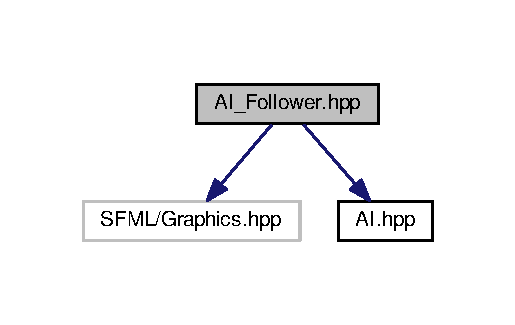
\includegraphics[width=247pt]{_a_i___follower_8hpp__incl}
\end{center}
\end{figure}
\subsection*{Classes}
\begin{DoxyCompactItemize}
\item 
class \hyperlink{class_a_i___follower}{A\+I\+\_\+\+Follower}
\begin{DoxyCompactList}\small\item\em Classe gérant l'\hyperlink{class_a_i}{A\+I} des ennemi qui sautent. \end{DoxyCompactList}\end{DoxyCompactItemize}


\subsection{Detailed Description}
\hyperlink{class_a_i}{A\+I} des enemy sautant. 

\begin{DoxyAuthor}{Author}
\{N. Guittonneau, P. Raballand\} 
\end{DoxyAuthor}
\begin{DoxyVersion}{Version}
1.\+0 
\end{DoxyVersion}
\begin{DoxyDate}{Date}
14/11/2015
\end{DoxyDate}
Gère les mouvement d'un \hyperlink{class_enemy}{Enemy} ayant pour base le mouvement de saut sur une \hyperlink{class_tile_map}{Tile\+Map} définie. Hérite du \hyperlink{class_a_i}{A\+I}. 
\hypertarget{_a_i___jumper_8hpp}{\section{A\+I\+\_\+\+Jumper.\+hpp File Reference}
\label{_a_i___jumper_8hpp}\index{A\+I\+\_\+\+Jumper.\+hpp@{A\+I\+\_\+\+Jumper.\+hpp}}
}


\hyperlink{class_a_i}{A\+I} des enemy sautant.  


{\ttfamily \#include $<$S\+F\+M\+L/\+Graphics.\+hpp$>$}\\*
{\ttfamily \#include \char`\"{}A\+I.\+hpp\char`\"{}}\\*
Include dependency graph for A\+I\+\_\+\+Jumper.\+hpp\+:
\nopagebreak
\begin{figure}[H]
\begin{center}
\leavevmode
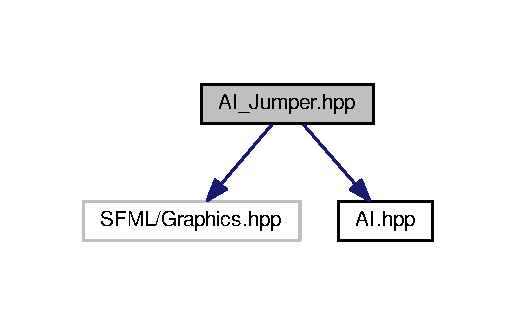
\includegraphics[width=247pt]{_a_i___jumper_8hpp__incl}
\end{center}
\end{figure}
\subsection*{Classes}
\begin{DoxyCompactItemize}
\item 
class \hyperlink{class_a_i___jumper}{A\+I\+\_\+\+Jumper}
\begin{DoxyCompactList}\small\item\em Classe gérant l'\hyperlink{class_a_i}{A\+I} des ennemi qui sautent. \end{DoxyCompactList}\end{DoxyCompactItemize}


\subsection{Detailed Description}
\hyperlink{class_a_i}{A\+I} des enemy sautant. 

\begin{DoxyAuthor}{Author}
\{N. Guittonneau, P. Raballand\} 
\end{DoxyAuthor}
\begin{DoxyVersion}{Version}
1.\+0 
\end{DoxyVersion}
\begin{DoxyDate}{Date}
14/11/2015
\end{DoxyDate}
Gère les mouvement d'un \hyperlink{class_enemy}{Enemy} ayant pour base le mouvement de saut sur une \hyperlink{class_tile_map}{Tile\+Map} définie. Hérite du \hyperlink{class_a_i}{A\+I}. 
\hypertarget{_a_i___land_base_8hpp}{\section{A\+I\+\_\+\+Land\+Base.\+hpp File Reference}
\label{_a_i___land_base_8hpp}\index{A\+I\+\_\+\+Land\+Base.\+hpp@{A\+I\+\_\+\+Land\+Base.\+hpp}}
}


\hyperlink{class_a_i}{A\+I} des enemy au sol.  


{\ttfamily \#include \char`\"{}A\+I.\+hpp\char`\"{}}\\*
Include dependency graph for A\+I\+\_\+\+Land\+Base.\+hpp\+:
\nopagebreak
\begin{figure}[H]
\begin{center}
\leavevmode
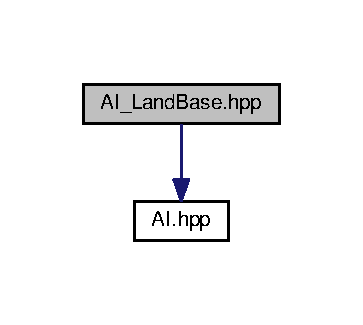
\includegraphics[width=174pt]{_a_i___land_base_8hpp__incl}
\end{center}
\end{figure}
\subsection*{Classes}
\begin{DoxyCompactItemize}
\item 
class \hyperlink{class_a_i___land_base}{A\+I\+\_\+\+Land\+Base}
\begin{DoxyCompactList}\small\item\em Classe gérant l'\hyperlink{class_a_i}{A\+I} des ennemi qui marchent. \end{DoxyCompactList}\end{DoxyCompactItemize}


\subsection{Detailed Description}
\hyperlink{class_a_i}{A\+I} des enemy au sol. 

\begin{DoxyAuthor}{Author}
\{N. Guittonneau, P. Raballand\} 
\end{DoxyAuthor}
\begin{DoxyVersion}{Version}
1.\+0 
\end{DoxyVersion}
\begin{DoxyDate}{Date}
14/11/2015
\end{DoxyDate}
Gère les mouvement d'un \hyperlink{class_enemy}{Enemy} ayant pour base le mouvement D/\+G au sol sur une \hyperlink{class_tile_map}{Tile\+Map} définie. Hérite du \hyperlink{class_a_i}{A\+I}. 
\hypertarget{_alive_entity_8hpp}{\section{Alive\+Entity.\+hpp File Reference}
\label{_alive_entity_8hpp}\index{Alive\+Entity.\+hpp@{Alive\+Entity.\+hpp}}
}


Classe définissant les objets \char`\"{}vivants\char`\"{}.  


{\ttfamily \#include $<$S\+F\+M\+L/\+Graphics.\+hpp$>$}\\*
Include dependency graph for Alive\+Entity.\+hpp\+:
\nopagebreak
\begin{figure}[H]
\begin{center}
\leavevmode
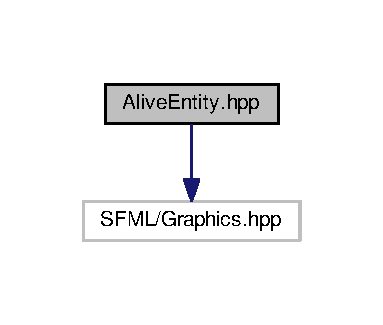
\includegraphics[width=184pt]{_alive_entity_8hpp__incl}
\end{center}
\end{figure}
This graph shows which files directly or indirectly include this file\+:
\nopagebreak
\begin{figure}[H]
\begin{center}
\leavevmode
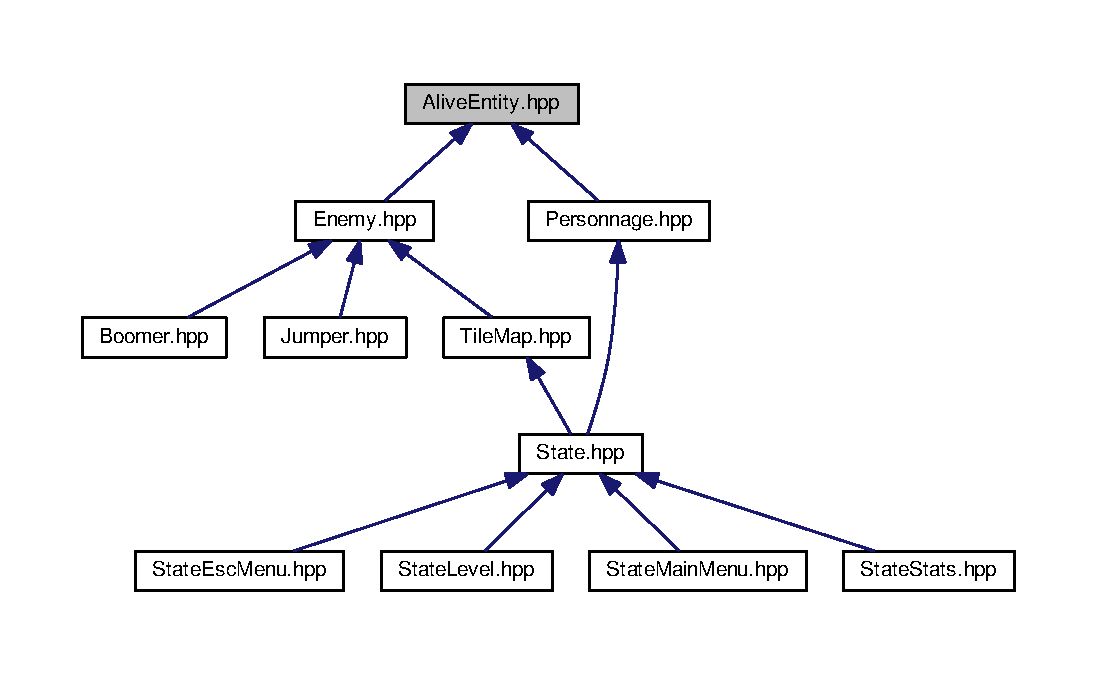
\includegraphics[width=350pt]{_alive_entity_8hpp__dep__incl}
\end{center}
\end{figure}
\subsection*{Classes}
\begin{DoxyCompactItemize}
\item 
class \hyperlink{class_alive_entity}{Alive\+Entity}
\begin{DoxyCompactList}\small\item\em Classe abstraite qui définissant les objets \char`\"{}vivants\char`\"{}. \end{DoxyCompactList}\end{DoxyCompactItemize}


\subsection{Detailed Description}
Classe définissant les objets \char`\"{}vivants\char`\"{}. 

\begin{DoxyAuthor}{Author}
\{N. Guittonneau, P. Raballand\} 
\end{DoxyAuthor}
\begin{DoxyVersion}{Version}
1.\+0 
\end{DoxyVersion}
\begin{DoxyDate}{Date}
14/11/2015
\end{DoxyDate}
Définit les méthodes communes à tout les objets \char`\"{}vivants\char`\"{} 
\hypertarget{_boomer_8hpp}{\section{Boomer.\+hpp File Reference}
\label{_boomer_8hpp}\index{Boomer.\+hpp@{Boomer.\+hpp}}
}


Classe des ennemis qui grossissent puis explosent.  


{\ttfamily \#include \char`\"{}Enemy.\+hpp\char`\"{}}\\*
Include dependency graph for Boomer.\+hpp\+:
\nopagebreak
\begin{figure}[H]
\begin{center}
\leavevmode
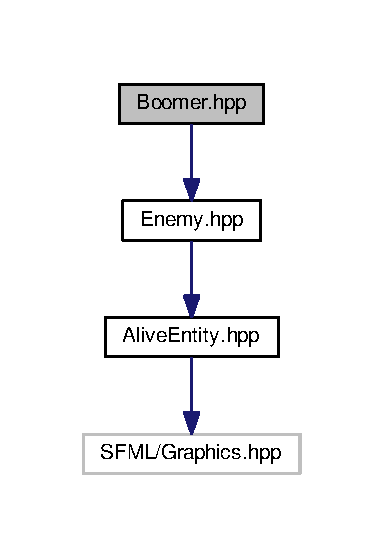
\includegraphics[width=184pt]{_boomer_8hpp__incl}
\end{center}
\end{figure}
\subsection*{Classes}
\begin{DoxyCompactItemize}
\item 
class \hyperlink{class_boomer}{Boomer}
\begin{DoxyCompactList}\small\item\em Classe gérant les ennemi qui explosent et se devisent. \end{DoxyCompactList}\end{DoxyCompactItemize}


\subsection{Detailed Description}
Classe des ennemis qui grossissent puis explosent. 

\begin{DoxyAuthor}{Author}
\{N. Guittonneau, P. Raballand\} 
\end{DoxyAuthor}
\begin{DoxyVersion}{Version}
1.\+0 
\end{DoxyVersion}
\begin{DoxyDate}{Date}
14/11/2015
\end{DoxyDate}
Définit un \hyperlink{class_enemy}{Enemy} pouvant exploser et se deviser Hérite de \hyperlink{class_enemy}{Enemy}. 
\hypertarget{_enemy_8hpp}{\section{Enemy.\+hpp File Reference}
\label{_enemy_8hpp}\index{Enemy.\+hpp@{Enemy.\+hpp}}
}


Classe définissant les ennemis.  


{\ttfamily \#include \char`\"{}Alive\+Entity.\+hpp\char`\"{}}\\*
Include dependency graph for Enemy.\+hpp\+:
\nopagebreak
\begin{figure}[H]
\begin{center}
\leavevmode
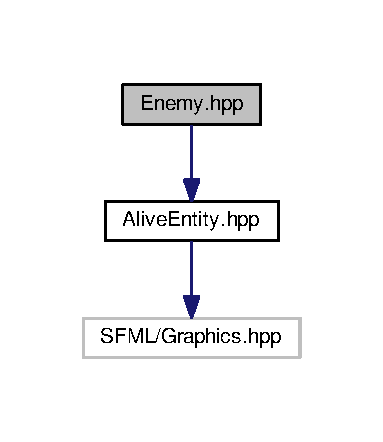
\includegraphics[width=184pt]{_enemy_8hpp__incl}
\end{center}
\end{figure}
This graph shows which files directly or indirectly include this file\+:
\nopagebreak
\begin{figure}[H]
\begin{center}
\leavevmode
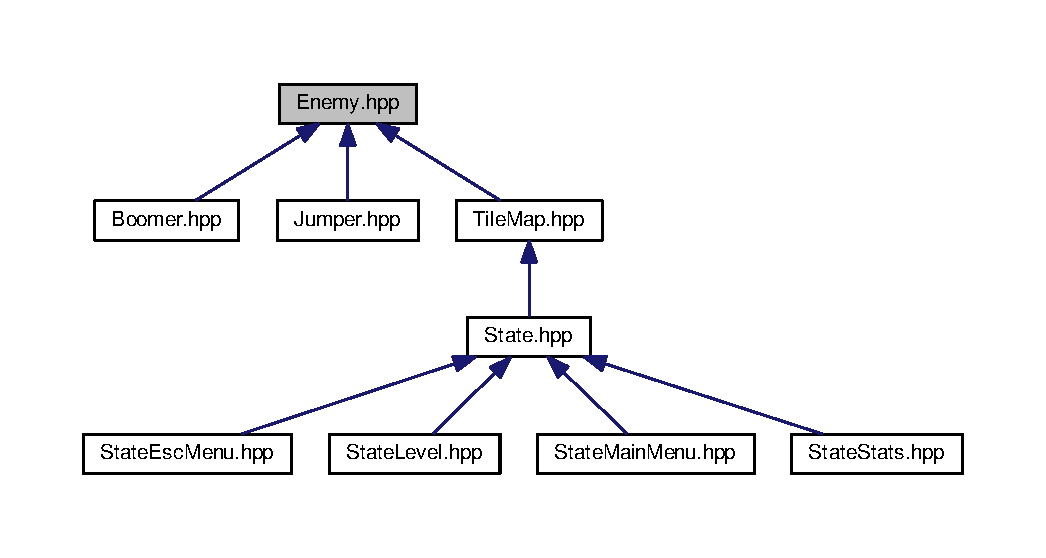
\includegraphics[width=350pt]{_enemy_8hpp__dep__incl}
\end{center}
\end{figure}
\subsection*{Classes}
\begin{DoxyCompactItemize}
\item 
class \hyperlink{class_enemy}{Enemy}
\begin{DoxyCompactList}\small\item\em Classe abstraite qui définissant les objets \char`\"{}vivants\char`\"{}. \end{DoxyCompactList}\end{DoxyCompactItemize}


\subsection{Detailed Description}
Classe définissant les ennemis. 

\begin{DoxyAuthor}{Author}
\{N. Guittonneau, P. Raballand\} 
\end{DoxyAuthor}
\begin{DoxyVersion}{Version}
1.\+0 
\end{DoxyVersion}
\begin{DoxyDate}{Date}
14/11/2015
\end{DoxyDate}
Définit les ennemis du \hyperlink{class_personnage}{Personnage}. Hérite de \hyperlink{class_alive_entity}{Alive\+Entity}. 
\hypertarget{_jeu_8hpp}{\section{Jeu.\+hpp File Reference}
\label{_jeu_8hpp}\index{Jeu.\+hpp@{Jeu.\+hpp}}
}


Gère l'ensemble des outils permettant d'effectuer une partie de Ducky\+Duck.  


{\ttfamily \#include $<$S\+F\+M\+L/\+Graphics.\+hpp$>$}\\*
Include dependency graph for Jeu.\+hpp\+:
\nopagebreak
\begin{figure}[H]
\begin{center}
\leavevmode
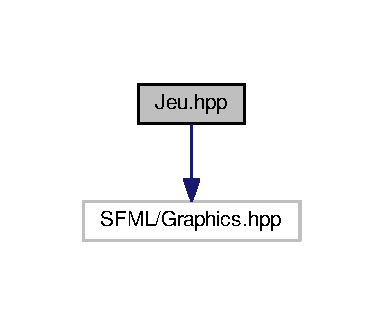
\includegraphics[width=184pt]{_jeu_8hpp__incl}
\end{center}
\end{figure}
This graph shows which files directly or indirectly include this file\+:
\nopagebreak
\begin{figure}[H]
\begin{center}
\leavevmode
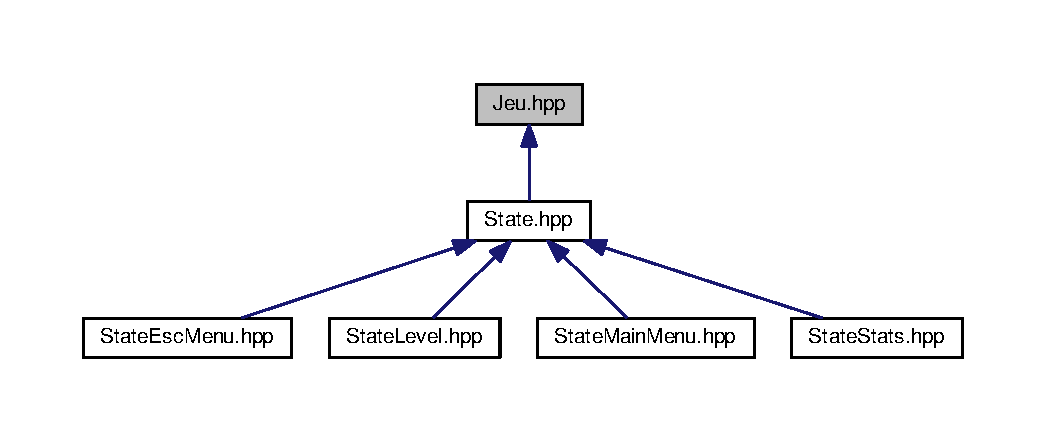
\includegraphics[width=350pt]{_jeu_8hpp__dep__incl}
\end{center}
\end{figure}
\subsection*{Classes}
\begin{DoxyCompactItemize}
\item 
class \hyperlink{class_jeu}{Jeu}
\begin{DoxyCompactList}\small\item\em Gère tout la fenêtre et les interactions lors d'une partie. \end{DoxyCompactList}\end{DoxyCompactItemize}


\subsection{Detailed Description}
Gère l'ensemble des outils permettant d'effectuer une partie de Ducky\+Duck. 

\begin{DoxyAuthor}{Author}
\{N. Guittonneau, P. Raballand\} 
\end{DoxyAuthor}
\begin{DoxyVersion}{Version}
1.\+0 
\end{DoxyVersion}
\begin{DoxyDate}{Date}
28/10/2015
\end{DoxyDate}
Gère tout la fenêtre et les interactions lors d'une partie 
\hypertarget{_jumper_8hpp}{\section{Jumper.\+hpp File Reference}
\label{_jumper_8hpp}\index{Jumper.\+hpp@{Jumper.\+hpp}}
}


Classe des ennemis marchant.  


{\ttfamily \#include \char`\"{}Enemy.\+hpp\char`\"{}}\\*
Include dependency graph for Jumper.\+hpp\+:
\nopagebreak
\begin{figure}[H]
\begin{center}
\leavevmode
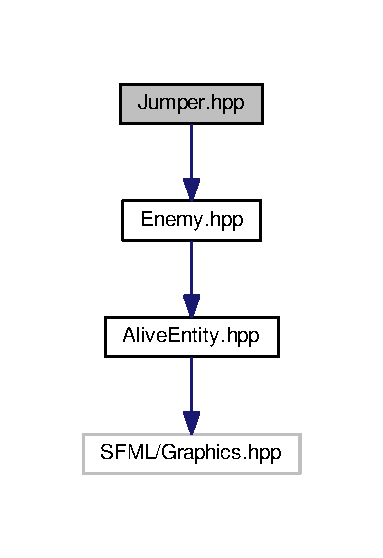
\includegraphics[width=184pt]{_jumper_8hpp__incl}
\end{center}
\end{figure}
\subsection*{Classes}
\begin{DoxyCompactItemize}
\item 
class \hyperlink{class_jumper}{Jumper}
\begin{DoxyCompactList}\small\item\em Classe gérant les ennemi qui marchent. \end{DoxyCompactList}\end{DoxyCompactItemize}


\subsection{Detailed Description}
Classe des ennemis marchant. 

\begin{DoxyAuthor}{Author}
\{N. Guittonneau, P. Raballand\} 
\end{DoxyAuthor}
\begin{DoxyVersion}{Version}
1.\+0 
\end{DoxyVersion}
\begin{DoxyDate}{Date}
14/11/2015
\end{DoxyDate}
Définit un \hyperlink{class_enemy}{Enemy} ne pouvant que marcher Hérite de \hyperlink{class_enemy}{Enemy}. 
\hypertarget{_personnage_8hpp}{\section{Personnage.\+hpp File Reference}
\label{_personnage_8hpp}\index{Personnage.\+hpp@{Personnage.\+hpp}}
}


Gère l'ensemble des outils neccessaires à l'éxécution des différentes méthodes du personnage.  


{\ttfamily \#include $<$S\+F\+M\+L/\+Graphics.\+hpp$>$}\\*
{\ttfamily \#include $<$Alive\+Entity.\+hpp$>$}\\*
Include dependency graph for Personnage.\+hpp\+:
\nopagebreak
\begin{figure}[H]
\begin{center}
\leavevmode
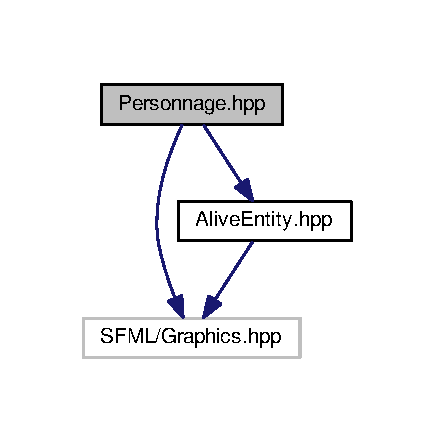
\includegraphics[width=208pt]{_personnage_8hpp__incl}
\end{center}
\end{figure}
This graph shows which files directly or indirectly include this file\+:
\nopagebreak
\begin{figure}[H]
\begin{center}
\leavevmode
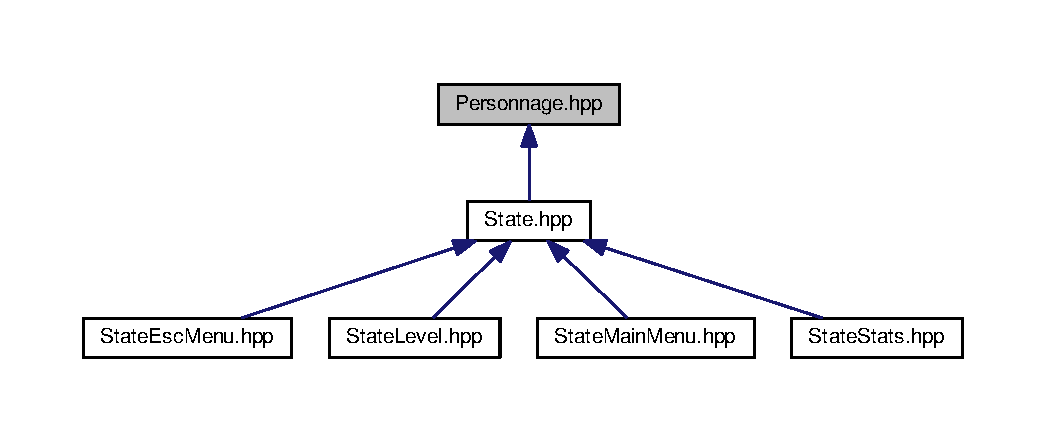
\includegraphics[width=350pt]{_personnage_8hpp__dep__incl}
\end{center}
\end{figure}
\subsection*{Classes}
\begin{DoxyCompactItemize}
\item 
class \hyperlink{class_personnage}{Personnage}
\begin{DoxyCompactList}\small\item\em Classe définissant un personnage. \end{DoxyCompactList}\end{DoxyCompactItemize}


\subsection{Detailed Description}
Gère l'ensemble des outils neccessaires à l'éxécution des différentes méthodes du personnage. 

\begin{DoxyAuthor}{Author}
\{N. Guittonneau,P. Raballand\} 
\end{DoxyAuthor}
\begin{DoxyVersion}{Version}
1.\+1 
\end{DoxyVersion}
\begin{DoxyDate}{Date}
29/10/2015
\end{DoxyDate}
Gère toutes les méthodes d'un personnage 
\hypertarget{_spawner_8hpp}{\section{Spawner.\+hpp File Reference}
\label{_spawner_8hpp}\index{Spawner.\+hpp@{Spawner.\+hpp}}
}


Créer une instance de \hyperlink{class_enemy}{Enemy}.  


\subsection*{Classes}
\begin{DoxyCompactItemize}
\item 
class \hyperlink{class_spawner}{Spawner}
\end{DoxyCompactItemize}


\subsection{Detailed Description}
Créer une instance de \hyperlink{class_enemy}{Enemy}. 

\begin{DoxyAuthor}{Author}
\{N. Guittonneau,P. Raballand\} 
\end{DoxyAuthor}
\begin{DoxyVersion}{Version}
1.\+0 
\end{DoxyVersion}
\begin{DoxyDate}{Date}
14/11/2015
\end{DoxyDate}
Gère le spawn du prototype (ennemi à cloner.) Pattern Prototype. 
\hypertarget{_state_8hpp}{\section{State.\+hpp File Reference}
\label{_state_8hpp}\index{State.\+hpp@{State.\+hpp}}
}


\hyperlink{class_state}{State}.  


{\ttfamily \#include \char`\"{}Tile\+Map.\+hpp\char`\"{}}\\*
{\ttfamily \#include \char`\"{}Personnage.\+hpp\char`\"{}}\\*
{\ttfamily \#include \char`\"{}Jeu.\+hpp\char`\"{}}\\*
Include dependency graph for State.\+hpp\+:
\nopagebreak
\begin{figure}[H]
\begin{center}
\leavevmode
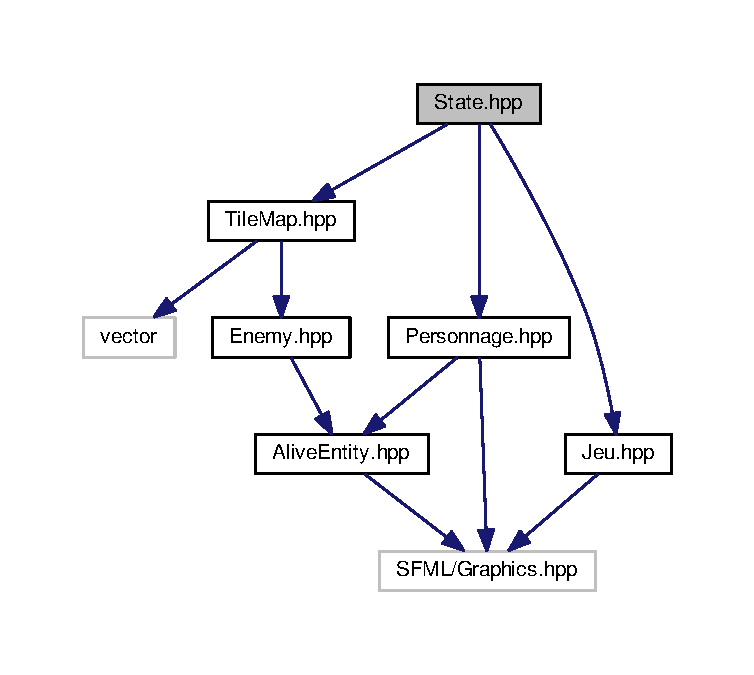
\includegraphics[width=350pt]{_state_8hpp__incl}
\end{center}
\end{figure}
This graph shows which files directly or indirectly include this file\+:
\nopagebreak
\begin{figure}[H]
\begin{center}
\leavevmode
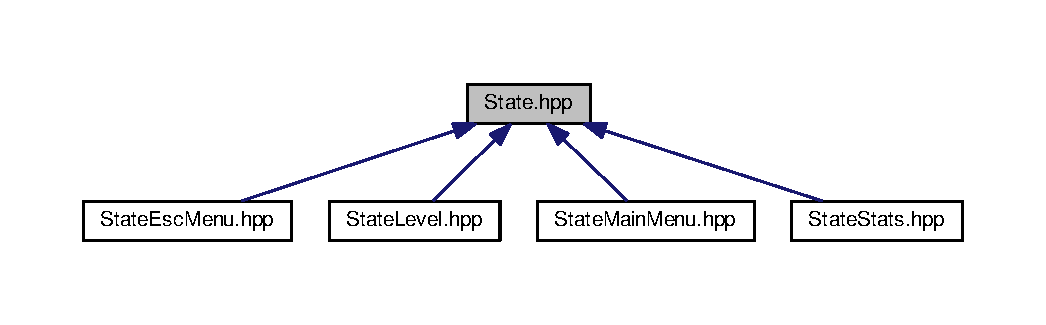
\includegraphics[width=350pt]{_state_8hpp__dep__incl}
\end{center}
\end{figure}
\subsection*{Classes}
\begin{DoxyCompactItemize}
\item 
class \hyperlink{class_state}{State}
\begin{DoxyCompactList}\small\item\em Interface du \hyperlink{class_state}{State}. \end{DoxyCompactList}\end{DoxyCompactItemize}


\subsection{Detailed Description}
\hyperlink{class_state}{State}. 

\begin{DoxyAuthor}{Author}
\{N. Guittonneau, P. Raballand\} 
\end{DoxyAuthor}
\begin{DoxyVersion}{Version}
1.\+0 
\end{DoxyVersion}
\begin{DoxyDate}{Date}
3/11/2015
\end{DoxyDate}
Interface du Pattern \hyperlink{class_state}{State} 
\hypertarget{_state_esc_menu_8hpp}{\section{State\+Esc\+Menu.\+hpp File Reference}
\label{_state_esc_menu_8hpp}\index{State\+Esc\+Menu.\+hpp@{State\+Esc\+Menu.\+hpp}}
}


Menu Pause du jeu.  


{\ttfamily \#include $<$S\+F\+M\+L/\+Graphics.\+hpp$>$}\\*
{\ttfamily \#include \char`\"{}State.\+hpp\char`\"{}}\\*
Include dependency graph for State\+Esc\+Menu.\+hpp\+:
\nopagebreak
\begin{figure}[H]
\begin{center}
\leavevmode
\includegraphics[width=350pt]{_state_esc_menu_8hpp__incl}
\end{center}
\end{figure}
\subsection*{Classes}
\begin{DoxyCompactItemize}
\item 
class \hyperlink{class_state_esc_menu}{State\+Esc\+Menu}
\begin{DoxyCompactList}\small\item\em Etat Esc\+Menu rattaché au Pattern \hyperlink{class_state}{State}. \end{DoxyCompactList}\end{DoxyCompactItemize}


\subsection{Detailed Description}
Menu Pause du jeu. 

\begin{DoxyAuthor}{Author}
\{N. Guittonneau, P. Raballand\} 
\end{DoxyAuthor}
\begin{DoxyVersion}{Version}
1.\+0 
\end{DoxyVersion}
\begin{DoxyDate}{Date}
3/11/2015
\end{DoxyDate}
Etat Esc\+Menu rattaché au Pattern \hyperlink{class_state}{State}. 
\hypertarget{_state_level_8hpp}{\section{State\+Level.\+hpp File Reference}
\label{_state_level_8hpp}\index{State\+Level.\+hpp@{State\+Level.\+hpp}}
}


Etat en jeu.  


{\ttfamily \#include $<$S\+F\+M\+L/\+Graphics.\+hpp$>$}\\*
{\ttfamily \#include \char`\"{}State.\+hpp\char`\"{}}\\*
Include dependency graph for State\+Level.\+hpp\+:
\nopagebreak
\begin{figure}[H]
\begin{center}
\leavevmode
\includegraphics[width=350pt]{_state_level_8hpp__incl}
\end{center}
\end{figure}
\subsection*{Classes}
\begin{DoxyCompactItemize}
\item 
class \hyperlink{class_state_level}{State\+Level}
\begin{DoxyCompactList}\small\item\em Etat \hyperlink{class_state_level}{State\+Level} rattaché au Pattern \hyperlink{class_state}{State}. \end{DoxyCompactList}\end{DoxyCompactItemize}


\subsection{Detailed Description}
Etat en jeu. 

\begin{DoxyAuthor}{Author}
\{N. Guittonneau, P. Raballand\} 
\end{DoxyAuthor}
\begin{DoxyVersion}{Version}
1.\+0 
\end{DoxyVersion}
\begin{DoxyDate}{Date}
3/11/2015
\end{DoxyDate}
Etat \hyperlink{class_state_level}{State\+Level} rattaché au Pattern \hyperlink{class_state}{State} 
\hypertarget{_state_main_menu_8hpp}{\section{State\+Main\+Menu.\+hpp File Reference}
\label{_state_main_menu_8hpp}\index{State\+Main\+Menu.\+hpp@{State\+Main\+Menu.\+hpp}}
}


Menu principal.  


{\ttfamily \#include $<$S\+F\+M\+L/\+Graphics.\+hpp$>$}\\*
{\ttfamily \#include \char`\"{}State.\+hpp\char`\"{}}\\*
Include dependency graph for State\+Main\+Menu.\+hpp\+:
\nopagebreak
\begin{figure}[H]
\begin{center}
\leavevmode
\includegraphics[width=350pt]{_state_main_menu_8hpp__incl}
\end{center}
\end{figure}
\subsection*{Classes}
\begin{DoxyCompactItemize}
\item 
class \hyperlink{class_state_main_menu}{State\+Main\+Menu}
\begin{DoxyCompactList}\small\item\em Etat Main\+Menu rattaché au Pattern \hyperlink{class_state}{State}. \end{DoxyCompactList}\end{DoxyCompactItemize}


\subsection{Detailed Description}
Menu principal. 

\begin{DoxyAuthor}{Author}
\{N. Guittonneau, P. Raballand\} 
\end{DoxyAuthor}
\begin{DoxyVersion}{Version}
1.\+0 
\end{DoxyVersion}
\begin{DoxyDate}{Date}
3/11/2015
\end{DoxyDate}
Etat Main\+Menu rattaché au Pattern \hyperlink{class_state}{State}. 
\hypertarget{_state_stats_8hpp}{\section{State\+Stats.\+hpp File Reference}
\label{_state_stats_8hpp}\index{State\+Stats.\+hpp@{State\+Stats.\+hpp}}
}


Affichage en fin de niveau.  


{\ttfamily \#include $<$S\+F\+M\+L/\+Graphics.\+hpp$>$}\\*
{\ttfamily \#include \char`\"{}State.\+hpp\char`\"{}}\\*
Include dependency graph for State\+Stats.\+hpp\+:
\nopagebreak
\begin{figure}[H]
\begin{center}
\leavevmode
\includegraphics[width=350pt]{_state_stats_8hpp__incl}
\end{center}
\end{figure}
\subsection*{Classes}
\begin{DoxyCompactItemize}
\item 
class \hyperlink{class_state_stats}{State\+Stats}
\begin{DoxyCompactList}\small\item\em Etat \hyperlink{class_state_stats}{State\+Stats} rattaché au Pattern \hyperlink{class_state}{State}. \end{DoxyCompactList}\end{DoxyCompactItemize}


\subsection{Detailed Description}
Affichage en fin de niveau. 

\begin{DoxyAuthor}{Author}
\{N. Guittonneau, P. Raballand\} 
\end{DoxyAuthor}
\begin{DoxyVersion}{Version}
1.\+0 
\end{DoxyVersion}
\begin{DoxyDate}{Date}
14/11/2015
\end{DoxyDate}
Etat \hyperlink{class_state_stats}{State\+Stats} rattaché au Pattern \hyperlink{class_state}{State}. 
\hypertarget{_tile_map_8hpp}{\section{Tile\+Map.\+hpp File Reference}
\label{_tile_map_8hpp}\index{Tile\+Map.\+hpp@{Tile\+Map.\+hpp}}
}


Gère les différentes interactions avec la map.  


{\ttfamily \#include $<$vector$>$}\\*
{\ttfamily \#include \char`\"{}Enemy.\+hpp\char`\"{}}\\*
Include dependency graph for Tile\+Map.\+hpp\+:
\nopagebreak
\begin{figure}[H]
\begin{center}
\leavevmode
\includegraphics[width=226pt]{_tile_map_8hpp__incl}
\end{center}
\end{figure}
This graph shows which files directly or indirectly include this file\+:
\nopagebreak
\begin{figure}[H]
\begin{center}
\leavevmode
\includegraphics[width=350pt]{_tile_map_8hpp__dep__incl}
\end{center}
\end{figure}
\subsection*{Classes}
\begin{DoxyCompactItemize}
\item 
class \hyperlink{class_tile_map}{Tile\+Map}
\begin{DoxyCompactList}\small\item\em Classe définissant un map. \end{DoxyCompactList}\end{DoxyCompactItemize}


\subsection{Detailed Description}
Gère les différentes interactions avec la map. 

\begin{DoxyAuthor}{Author}
\{N. Guittonneau, P. Raballand\} 
\end{DoxyAuthor}
\begin{DoxyVersion}{Version}
1.\+0 
\end{DoxyVersion}
\begin{DoxyDate}{Date}
29/10/2015
\end{DoxyDate}
Gère toutes les interactions avec la carte joué par le jeu. 
%--- End generated contents ---

% Index
\newpage
\phantomsection
\addcontentsline{toc}{chapter}{Index}
\printindex

\end{document}
